% Course report: Agent-Driven Design Space Exploration for HLS Acceleration of
% SRCNN on the Kria KV260.  Converted from the Notion page of the same name.
%
% Build (any one of):
%   tectonic main.tex                 (XeTeX engine, used for the checked build)
%   latexmk -xelatex main.tex
%   latexmk -pdf main.tex             (pdfLaTeX; needs the TeX Gyre fonts, standard in TeX Live / Overleaf)
%
% Layout: sections/ holds one file per chapter, figures/ the images, code/ the
% two source listings reproduced in the appendices.  Comment out the appendix
% \input / \lstinputlisting lines at the end to shorten the PDF.

% Layout switch: \compacttrue gives the dense layout (10pt, 2 cm margins, smaller
% figures); \compactfalse the roomier one (11pt, 2.4 cm margins).
\newif\ifcompact
\compacttrue
\ifcompact\documentclass[10pt,a4paper]{article}\else\documentclass[11pt,a4paper]{article}\fi

% ---------------------------------------------------------------- fonts
\usepackage{iftex}
\ifPDFTeX
  \usepackage[T1]{fontenc}
  \usepackage[utf8]{inputenc}
  \usepackage{textcomp}
  \usepackage{tgpagella}
  \usepackage{tgheros}
  \usepackage[scaled=0.85]{beramono}
\else
  \usepackage{fontspec}
  \setmainfont{texgyrepagella}[Extension=.otf,UprightFont=*-regular,BoldFont=*-bold,
    ItalicFont=*-italic,BoldItalicFont=*-bolditalic]
  \setsansfont{texgyreheros}[Extension=.otf,UprightFont=*-regular,BoldFont=*-bold,
    ItalicFont=*-italic,BoldItalicFont=*-bolditalic]
  \setmonofont{lmmonolt10}[Extension=.otf,UprightFont=*-regular,BoldFont=*-bold,
    ItalicFont=*-oblique,BoldItalicFont=*-boldoblique,Scale=MatchLowercase]
\fi

% ---------------------------------------------------------------- packages
\ifcompact\usepackage[a4paper,margin=2cm,top=2cm,bottom=2.2cm]{geometry}\else\usepackage[a4paper,margin=2.4cm]{geometry}\fi
\usepackage{amsmath,amssymb}
\usepackage{graphicx}
\usepackage{booktabs}
\usepackage{tabularx}
\usepackage{longtable}
\usepackage{array}
\usepackage{pdflscape}
\usepackage{caption}
\usepackage{listings}
\usepackage{xcolor}
\usepackage{enumitem}
\usepackage{microtype}
\usepackage{titlesec}
\ifcompact\titlespacing*{\section}{0pt}{1.6ex plus .4ex}{0.8ex}\titlespacing*{\subsection}{0pt}{1.2ex plus .3ex}{0.5ex}\titlespacing*{\subsubsection}{0pt}{1ex plus .2ex}{0.4ex}\setlength{\textfloatsep}{8pt plus 2pt}\setlength{\intextsep}{8pt plus 2pt}\setlength{\floatsep}{6pt}\renewcommand{\topfraction}{0.9}\renewcommand{\bottomfraction}{0.7}\renewcommand{\textfraction}{0.1}\renewcommand{\floatpagefraction}{0.8}\fi
\usepackage{calc}
\usepackage[hidelinks,unicode]{hyperref}
% commands pandoc emits for the skill appendix
\providecommand{\tightlist}{\setlength{\itemsep}{0pt}\setlength{\parskip}{0pt}}
\providecommand{\passthrough}[1]{#1}
\providecommand{\real}[1]{#1}

\graphicspath{{./}}
\ifcompact\newcommand{\figscale}{0.78}\else\newcommand{\figscale}{1}\fi
\newcommand{\figw}{\dimexpr\figscale\linewidth\relax}
\newcommand{\figh}{\dimexpr\figscale\textheight\relax}
\ifPDFTeX\pdfminorversion=7\else\special{pdf:minorversion 7}\fi
\captionsetup{font=small,labelfont=bf,width=0.95\linewidth}
\ifcompact\captionsetup{font=footnotesize,skip=4pt}\renewcommand{\arraystretch}{1.0}\fi
\ifcompact\setlist{itemsep=0pt,topsep=2pt,parsep=0pt}\else\setlist{itemsep=2pt,topsep=4pt}\fi
\newcolumntype{C}[1]{>{\centering\arraybackslash}p{#1}}
\newcolumntype{R}[1]{>{\raggedleft\arraybackslash}p{#1}}
\newcolumntype{L}[1]{>{\raggedright\arraybackslash}p{#1}}
\newcolumntype{Y}{>{\raggedright\arraybackslash}X}
\urlstyle{tt}
\makeatletter\g@addto@macro{\UrlBreaks}{\do\/\do\_\do\-\do\.}\makeatother
\ifcompact\setlength{\parskip}{0pt}\else\setlength{\parskip}{0.35em}\fi
\setlength{\emergencystretch}{2em}
\setlength{\tabcolsep}{4pt}
\ifcompact\else\renewcommand{\arraystretch}{1.12}\fi
\pdfstringdefDisableCommands{\def\times{x}\def\rightarrow{->}}

% ---------------------------------------------------------------- listings
\definecolor{lstbg}{gray}{0.96}
\definecolor{lstcomment}{rgb}{0.30,0.45,0.30}
\definecolor{lstkw}{rgb}{0.10,0.20,0.60}
\lstset{
  basicstyle=\ttfamily\footnotesize,
  backgroundcolor=\color{lstbg},
  commentstyle=\color{lstcomment},
  keywordstyle=\color{lstkw},
  frame=single, framerule=0pt, framesep=4pt,
  breaklines=true, breakatwhitespace=true,
  columns=fullflexible, keepspaces=true,
  showstringspaces=false, tabsize=4,
  captionpos=b, extendedchars=true,
  numbers=none,
  literate=
    {·}{{$\cdot$}}1 {×}{{$\times$}}1 {→}{{$\rightarrow$}}1 {↔}{{$\leftrightarrow$}}1
    {−}{{$-$}}1 {≤}{{$\le$}}1 {≥}{{$\ge$}}1 {ᵀ}{{\textsuperscript{T}}}1
    {²}{{\textsuperscript{2}}}1 {½}{{\textonehalf}}1,
}
\lstdefinestyle{source}{
  language=C++,
  basicstyle=\ttfamily\scriptsize,
  numbers=left, numberstyle=\tiny\color{gray}, numbersep=6pt, stepnumber=5, firstnumber=1,
  morekeywords={ap_int,ap_uint,ap_fixed,hls,stream,constexpr,static_assert},
}

% ---------------------------------------------------------------- metadata
\title{\textbf{Agent-Driven Design Space Exploration for HLS Acceleration of SRCNN on the Kria KV260}}
\author{Xiufu Sun (1372750) \and Puze Li (1741640)}
\date{October 2026}

\begin{document}

\maketitle
\tableofcontents
\clearpage

% Generated from the Notion page by tools/notion2tex.py (see report/README.md).
\section{Introduction}\label{sec:1}

Single-image super-resolution (SR) reconstructs a high-resolution image from one low-resolution input \cite{ref1}. SRCNN \cite{ref2,ref3} was the first convolutional network to do this end to end and remains the simplest learned SR method: three convolutional layers applied to a bicubically upscaled image, trained to minimise the mean squared error against the high-resolution original. On the standard Set5 and Set14 benchmarks \cite{ref5,ref6} it improves the peak signal-to-noise ratio (PSNR) of the bicubic input by 1 to 3 dB depending on the image (Table~\ref{tab:13}).

\textbf{The algorithm.} Figure~\ref{fig:network} shows the network. The first layer extracts features with 64 kernels of 9$\times$9 on the single-channel input, the second maps them non-linearly with 32 kernels of 1$\times$1, and the third reconstructs one output channel with a 5$\times$5 kernel; the first two layers are followed by ReLU, the last is linear \cite{ref7}. Conv1 and Conv3 pad by edge replication so that the output has the same size as the input \cite{ref8}. The model is small, 8,129 parameters in all, but a single 255$\times$255 frame costs 522 million multiply-accumulate (MAC) operations, of which Conv1 alone is 64.5 \% (Table~\ref{tab:4}). This combination, a tiny parameter set and a large, perfectly regular arithmetic load with abundant data reuse between neighbouring pixels, is what makes a convolutional network a good match for an FPGA \cite{ref10}: the weights fit on chip, the computation can be unrolled across DSP slices, and the intermediate data never has to leave the device.

\begin{figure}[!htbp]
\centering
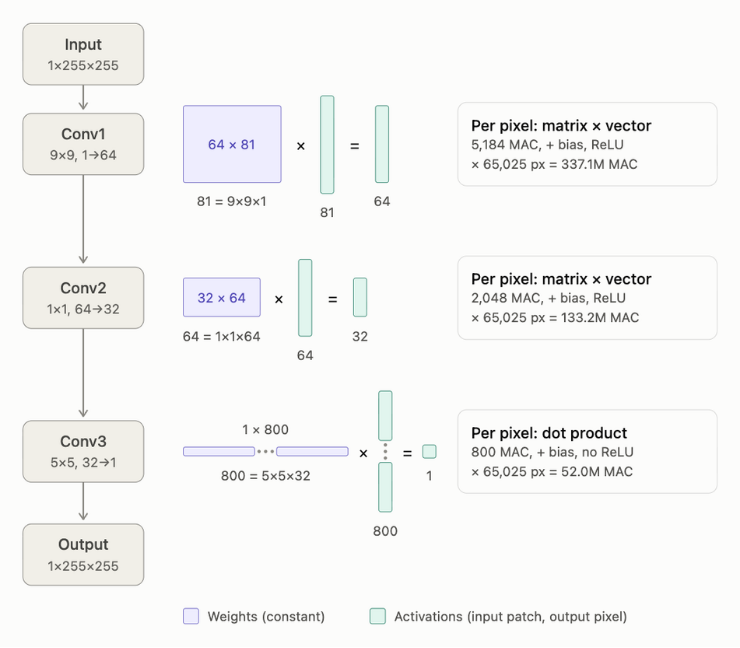
\includegraphics[width=0.78\figw]{figures/fig00-network.png}
\caption{The SRCNN network as implemented: Conv1 (9$\times$9, 1$\rightarrow$64 channels, ReLU), Conv2 (1$\times$1, 64$\rightarrow$32, ReLU) and Conv3 (5$\times$5, 32$\rightarrow$1, linear) on a 255$\times$255 single-channel input. Per output pixel each layer is a matrix--vector product with 5,184, 2,048 and 800 multiply-accumulates; over the 65,025 pixels of a frame that is 337.1 M, 133.2 M and 52.0 M, 522 million in all.}
\label{fig:network}
\end{figure}

\textbf{Platform and tool flow.} The target is the AMD Kria KV260 Vision AI Starter Kit \cite{ref11}, whose Zynq UltraScale+ MPSoC (device xck26-sfvc784-2LV-c) offers 1,248 DSP48E2 slices, 117,120 LUTs, 234,240 flip-flops, 5.1 Mb of block RAM and 18 Mb of UltraRAM in the programmable logic, next to a quad-core Arm processing system with DDR4. The accelerator is written in C++ and synthesised with Vitis HLS \cite{ref12}, integrated with the processing system in Vivado, and driven from Python through PYNQ \cite{ref13}.

\textbf{Goals.} Four goals were fixed at the start of the optimisation phase and are used as the specification against which Sections~\ref{sec:5} and \ref{sec:6} measure the result:

\begin{itemize}
\item \textbf{G1, function.} The accelerator keeps the original interface (the \texttt{srcnn} function with float arrays and parameters loaded from memory at run time), the 1-64-32-1 network and replicate padding. Its output must be bit-exact against a fixed-point reference on every one of the 13 Set14 images, and the mean PSNR of that reference on Set14 may be no more than 0.1 dB below the floating-point network.
\item \textbf{G2, speed.} The primary metric is milliseconds per 255$\times$255 frame, measured on the board. The goal is to make it as small as possible; no fixed target was set, because at the outset we had no basis for one beyond the baseline.
\item \textbf{G3, fit.} The design must place, route and meet timing on the xck26 device as an integrated PS+PL system.
\item \textbf{G4, evidence.} Every number reported must be traceable to an archived run, with its level of evidence stated: HLS estimate, RTL co-simulation, post-route implementation or on-board measurement.
\end{itemize}

\textbf{Approach.} The work has three stages. We first wrote a tiled, pipelined floating-point implementation of the original algorithm and verified it on the board (Section~\ref{sec:2}). It is correct and slow, and its profile shows why: the three layers run one after another, almost all DSP slices are idle, and all arithmetic is in single-precision float. Closing that gap is a search over a large space of HLS techniques, and each point in the space costs tens of minutes of synthesis and up to three hours of place-and-route to evaluate. Rather than search by hand, we handed the loop to general-purpose LLM coding agents (OpenAI Codex and Anthropic Claude Code) operating under a written experimental protocol: a fixed functional contract, one primary metric, explicit acceptance gates, an experiment card committed before every run, and an archive of every result including failures. We wrote the plans and reviewed the results; the agents wrote, ran and documented the experiments (Section~\ref{sec:3}). The design that emerged, a whole-network dataflow pipeline in 10-bit fixed point with Winograd convolution \cite{ref15,ref16} on Conv1 and two-products-per-DSP packing on Conv2, is explained decision by decision in Section~\ref{sec:4}. Finally, the IP was integrated, verified on the board and profiled, and the difference between its simulated and measured speed was traced to its causes (Section~\ref{sec:5}).

\textbf{Contributions.} The report makes three. First, a verified SRCNN accelerator whose on-board hardware time per frame falls from 2.238 s for the baseline to 2.938 ms, bit-exact against its fixed-point reference on every test image. Second, an auditable protocol for using general coding agents to search an HLS design space, with the finding that for this network the HLS logic estimates are pessimistic by about 2$\times$ and the clock estimates optimistic by about 2$\times$, so that a search ranked on HLS estimates would have chosen the wrong design. Third, a measured account of the gap between RTL simulation and the board, attributed with hardware counters to the clock configuration and to single-beat AXI reads on the input path.

The remainder of the report is organised as follows. Section~\ref{sec:2} analyses the algorithm and the baseline. Section~\ref{sec:3} describes the agent-driven exploration: the protocol, what it caught, and the decisions that shaped the search. Section~\ref{sec:4} explains the final architecture layer by layer. Section~\ref{sec:5} covers Vivado integration, on-board verification and performance debugging. Section~\ref{sec:6} discusses the results against the goals, the sources of the speedup, the method, and its limitations; Section~\ref{sec:7} concludes.

% Generated from the Notion page by tools/notion2tex.py (see report/README.md).
\section{Baseline and Algorithm Analysis}\label{sec:2}

The algorithm consists of three convolutional layers:

\begin{itemize}
\item Conv1 -- Feature Extraction: The first layer applies 64 convolution kernels of size 9$\times$9 to extract local image features, followed by a ReLU activation function.
\item Conv2 -- Nonlinear Mapping: The second layer uses 1$\times$1 convolutions to combine the extracted features and generate 32 feature maps, followed by another ReLU activation function.
\item Conv3 -- Image Reconstruction: The final layer applies 5$\times$5 convolutions to reconstruct the output image. No activation function is applied after this layer.
\end{itemize}

\subsection{Feasibility of FPGA Acceleration}\label{sec:2.1}

This structure is well suited for FPGA acceleration because it exhibits repetitive computation, parallelism, and data reuse. First, convolution requires a large number of multiply-accumulate (MAC) operations. For the 255$\times$255 input used in this project, the three layers require approximately 522 million MAC operations in the original computation. Second, different output channels and spatial positions can be computed independently, allowing multiple processing units to work in parallel. Loop unrolling can exploit this parallelism to increase the number of MAC operations executed per cycle. Third, convolution offers significant data reuse. The same weights are applied at multiple image positions, and input pixels contribute to multiple output features. By storing frequently accessed data on-chip, repeated external memory accesses can be reduced.

Based on these characteristics, the baseline implementation uses several HLS optimization directives, listed in Table~\ref{tab:1}.

\begin{table}[!htbp]
\centering
\footnotesize
\caption{HLS directives used in the baseline implementation and their function.}
\label{tab:1}
\begin{tabularx}{\linewidth}{lY}
\toprule
HLS Directive & Function \\
\midrule
\texttt{PIPELINE} & Overlaps consecutive loop iterations \\
\texttt{UNROLL} & Increases parallel computation across loop iterations \\
\texttt{ARRAY\_PARTITION} & Enables parallel access \\
\texttt{BIND\_STORAGE} & Specifies how on-chip storage resources are used \\
\texttt{INTERFACE} & Defines the control interface and external memory connections \\
\bottomrule
\end{tabularx}
\end{table}

\subsubsection{Baseline deployment and validation on board}\label{sec:2.1.1}

The first problem was storage capacity. The original HLS estimate required over 10,000 BRAMs, far exceeding the resources available on the board. So, we adopted tiling with a size of 16$\times$16, and added channel parallelism and pipelining. After optimization, the HLS-estimated BRAM usage dropped to 151, and the cycle count was reduced by about 30 times. The corresponding cost is an increase in MACs.

The baseline was validated using 13 test images from the Set14 test dataset. The resulting MSE was \texttt{3.166 $\times$ 10\textsuperscript{-14}}. The average execution time on the board was approximately 2.238 seconds per frame, corresponding to a throughput of 0.447 frames per second (FPS).

\subsubsection{Limitations of the Baseline}\label{sec:2.1.2}

Despite the baseline verified the correctness of the algorithm on the FPGA, it still has limitations. First, the three convolutional layers execute sequentially. Although some inner loops achieved an initiation interval (II) of 1, the convolutional layers are still executed in sequence. We will consider introducing a streaming interface and task-level dataflow in subsequent work to reduce intermediate storage and allow computations of different convolutional layers to run concurrently. Second, Conv1 and Conv3 together account for approximately 82\% of the execution time, while the baseline uses only about 3.69\% of the available DSP resources. This indicates that more parallel computation can be designed for the first and third layers. Third, the baseline runs at a relatively low clock frequency. As long as the design continues to meet timing constraints, we can increase the clock frequency to further improve execution speed. Finally, reducing numerical precision and optimizing data representation will also improve resource efficiency and enable higher parallelism. We will follow this direction for subsequent optimization.

% Generated from the Notion page by tools/notion2tex.py (see report/README.md).
\section{Agent-Driven Design Space Exploration}\label{sec:3}

\subsection{Why an agent}\label{sec:3.1}

Optimizing an HLS accelerator is a search. Every iteration follows the same fixed loop: choose one optimization, change the code, run C simulation, run HLS synthesis, read the reports, and, for promising candidates, run C/RTL co-simulation and Vivado place-and-route. The loop is slow (one synthesis of this design takes 10 to 60 minutes on our host and one implementation up to three hours), the reports are long, and the space of techniques is large: precision, tiling, line buffers, loop pipelining and unrolling, dataflow, DSP packing, Winograd, parameter storage, FIFO depths and clock targets can be combined in countless ways. As beginners without hardware intuition we could not pick the right combination directly, and we could not afford to try many combinations by hand.

Both Vitis HLS and Vivado expose complete command-line flows, so the loop can be driven by a program. We therefore handed the loop to general-purpose LLM coding agents (OpenAI Codex and Anthropic Claude Code) running on a laptop and executing the tools over SSH on a Linux host (12 logical CPUs, 15 GiB of memory) with the Xilinx installation. This section describes how the agents were controlled, what the resulting search looked like, what the method caught that we would otherwise have missed, and which decisions were made by humans. The hardware results themselves are analyzed in Section~\ref{sec:4}.

\subsection{The problem was not the model}\label{sec:3.2}

Our first attempts showed that a capable model is not enough. Left alone, an agent tends to:

\begin{itemize}
\item change several things at once, so that a measured gain cannot be attributed to any one of them;
\item explain results after the fact, adjusting its expectation to whatever the tool reported;
\item present a weaker result as a stronger one, for example reporting an HLS latency estimate as if it were the frame time, or a functional pass as a speedup;
\item lose track of what has already been tried over a session that lasts many hours.
\end{itemize}

None of these are failures of hardware knowledge. They are failures of experimental discipline, and they are the same failures a student makes. Mature frameworks now exist for constraining a model and automating its workflow. Building on Claude Code, we wrote the discipline down as a rules file (\texttt{AGENTS.md}) and a reusable skill file that the agent loads at the start of every session; Figure~\ref{fig:1} shows an excerpt. The rest of this section is that method.

\begin{figure}[!htbp]
\centering
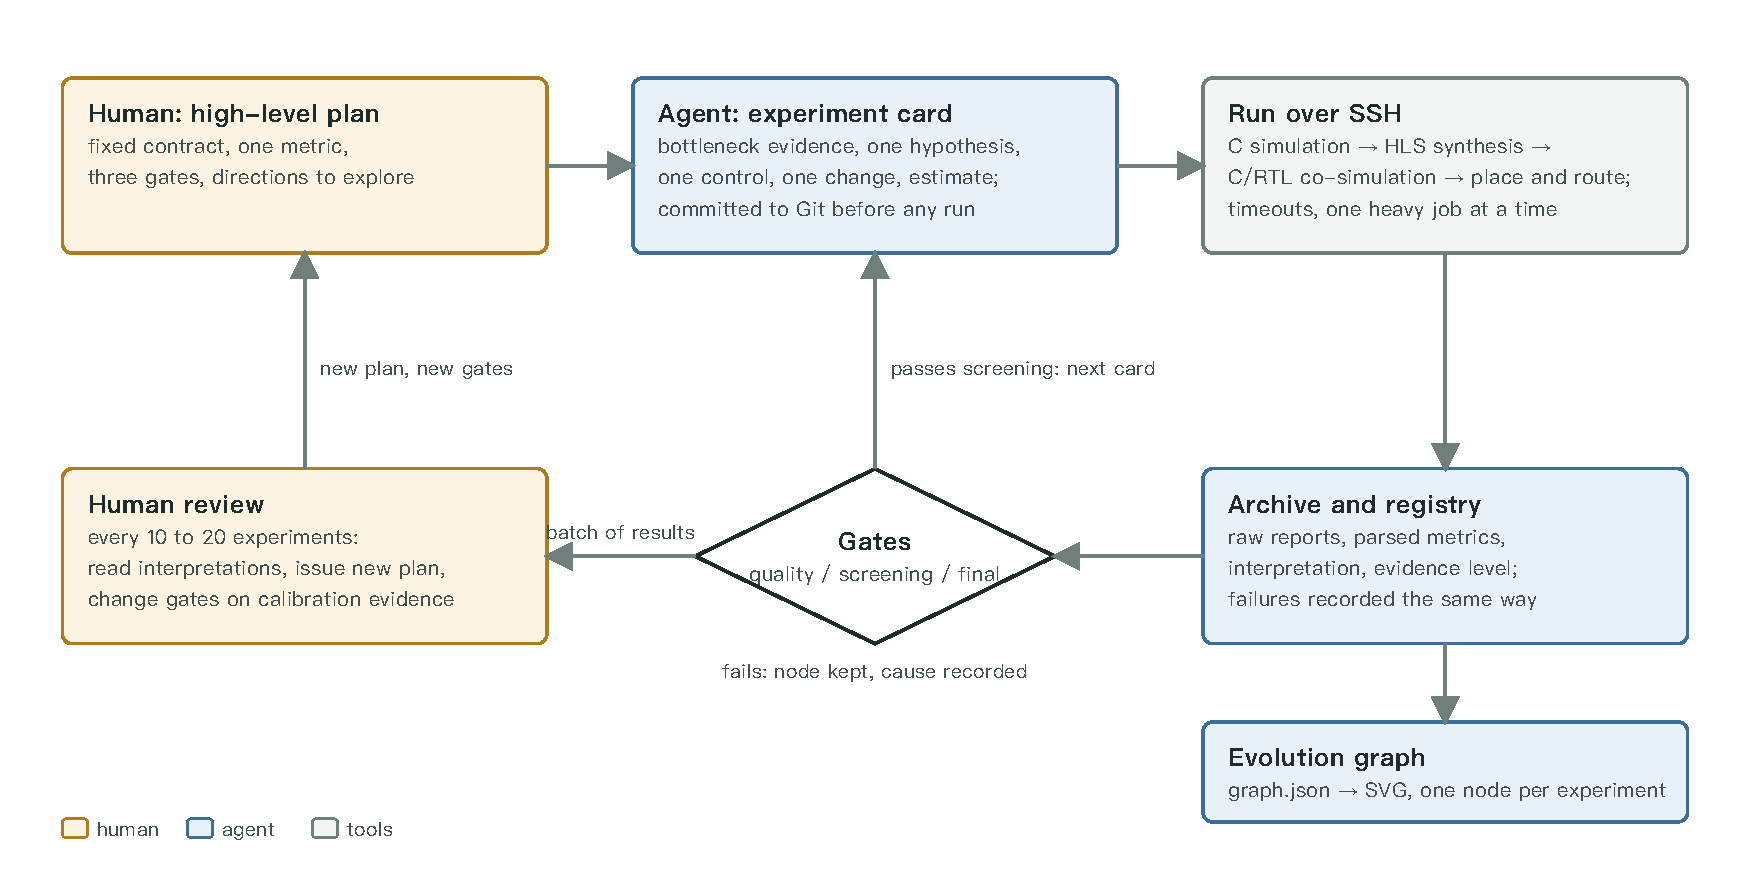
\includegraphics[width=0.9\figw]{figures/fig01-experiment-loop.pdf}
\caption{Excerpt of the rules file (AGENTS.md) loaded by the coding agent at the start of every session, which fixes the experimental discipline described in this section.}
\label{fig:1}
\end{figure}

\subsection{The protocol}\label{sec:3.3}

\textbf{Plan before experimenting.} Planning happens at two levels. A high-level plan (\texttt{docs/\allowbreak{}000N-*.md}) fixes what must not change, what is being optimized, and which directions to explore. For this project the fixed contract is: the \texttt{srcnn} function signature with float arrays, runtime-loaded parameters, replicate padding, the 1-64-32-1 network, and bit-exact agreement with a fixed-point reference on all 13 Set14 images. The single primary metric is milliseconds per frame, computed as cycles multiplied by clock period. Three gates separate ``ran'' from ``counts''; they are defined in Table~\ref{tab:2}.

\begin{table}[!htbp]
\centering
\footnotesize
\caption{The three acceptance gates of the exploration protocol and the concrete criterion used for each in this project.}
\label{tab:2}
\begin{tabularx}{\linewidth}{lp{3.4cm}Y}
\toprule
Gate & Question & Criterion used in this project \\
\midrule
Quality & Is the output correct? & Bit-exact against the 10-bit \texttt{ap\_fixed} reference E017 (or the mixed-precision reference E065) on every image; mean PSNR change on Set14 no worse than -0.1 dB \\
Screening & Is it worth verifying further? & HLS synthesis completes with II = 1 in the compute loops and resources inside an explicit screen (for the T4 designs: DSP $\le$ 1100, LUT $\le$ 170 k, FF $\le$ 230 k) \\
Final & Can we call it feasible? & Post-route timing met at the implemented clock, zero unrouted nets, routed resources within the device, and C/RTL co-simulation bit-exact over two or more frames with finite FIFOs \\
\bottomrule
\end{tabularx}
\end{table}

Only designs that pass the final gate enter the ranking. We review the completed experiments and issue a new high-level plan; the agent does not change the gates itself.

\textbf{Register before running.} Every experiment gets an immutable ID (E, P, W, G, S, C, F series by direction) and a card that is committed to Git before any tool runs. The card contains the bottleneck evidence (a specific line of a specific report), one hypothesis, one control experiment, the single thing changed relative to the control, and a paper estimate of DSP, BRAM, LUT, FF and cycles with its derivation. Because the card is committed first, the estimate cannot be adjusted afterwards. Listing~\ref{lst:1} shows the relevant part of one card.

\begin{lstlisting}[caption={Experiment card C13 (excerpt), planned 2026-10-12T04:58 UTC, control W21.},label={lst:1},language={}]
Change: T=4 fold; Conv2 only switches to E065's signed 8-bit weights, two coefficients
        pre-packed per 27-bit DSP operand once per frame; everything else frozen.
Paper estimate: DSP 1032 (576+256+200), BRAM18K 146, LUT 150000, FF 220000,
        latency 292000 cycles.  Basis: 2304/4 Conv1, 2048/(4*2) Conv2 pairs, 800/4 Conv3;
        C11 measured 1036 DSP / 198436 LUT / 231297 FF with the old loader.
Measured (HLS): DSP 1032, BRAM18K 146, LUT 127966 (-14.7 %), FF 192308 (-12.6 %),
        263090 cycles (-9.9 %).  All deviations within 20 %.
\end{lstlisting}

\textbf{Record everything, with an evidence level.} Each run is archived under \texttt{experiments/\allowbreak{}<ID>\_\allowbreak{}<name>/\allowbreak{}} with the card, the source snapshot, the raw logs, the parsed reports and a one-page interpretation. Failed, timed-out and invalid runs are archived in the same way; 100 of the 231 registered experiments ended in \texttt{fail}, \texttt{infeasible}, \texttt{invalid\_config} or \texttt{timeout}. The registry \texttt{results.csv} is generated by a parser from the reports and is never edited by hand. Every number carries its evidence level, in increasing order of strength:

\begin{quote}
paper estimate $\rightarrow$ C simulation $\rightarrow$ HLS synthesis estimate $\rightarrow$ C/RTL co-simulation $\rightarrow$ post-route implementation $\rightarrow$ on-board measurement
\end{quote}

The agent may not present a lower level as a higher one. The log records the rule being applied: ``a functional PASS is not a speedup'' (F45), ``a slack-derived period is not a verified clock'' (W22), ``the clock and the thread count changed together, so the runtime change cannot be credited to threads''. In practice this rule is what forced us to notice that HLS estimates are systematically wrong for this design (see the decisions below).

\textbf{Draw the evolution graph and hand over.} Later experiments build on the results or hypotheses of earlier ones, so the experiments form a directed graph. The agent maintains \texttt{graph.json} with one node per experiment and one edge per dependency (design lineage, retry after fix, integration, numerical evidence, control, verification), and a script renders it. At the end of each session a progress file records the current branch, the running jobs, the open decisions and how to resume, so that a new session or a different model can continue without re-deriving the state.

\subsection{The search as a whole}\label{sec:3.4}

The agents registered 231 experiments over 71 design directories; the registry timestamps run from 2026-10-10 to 2026-10-13, with the baseline setup starting on 2026-09-29. 20 experiments reached Vivado implementation and 16 reached C/RTL co-simulation. Figure~\ref{fig:2} condenses the search to its 51 turning points; the complete graph and the per-route views are in the repository.

\begin{figure}[!htbp]
\centering
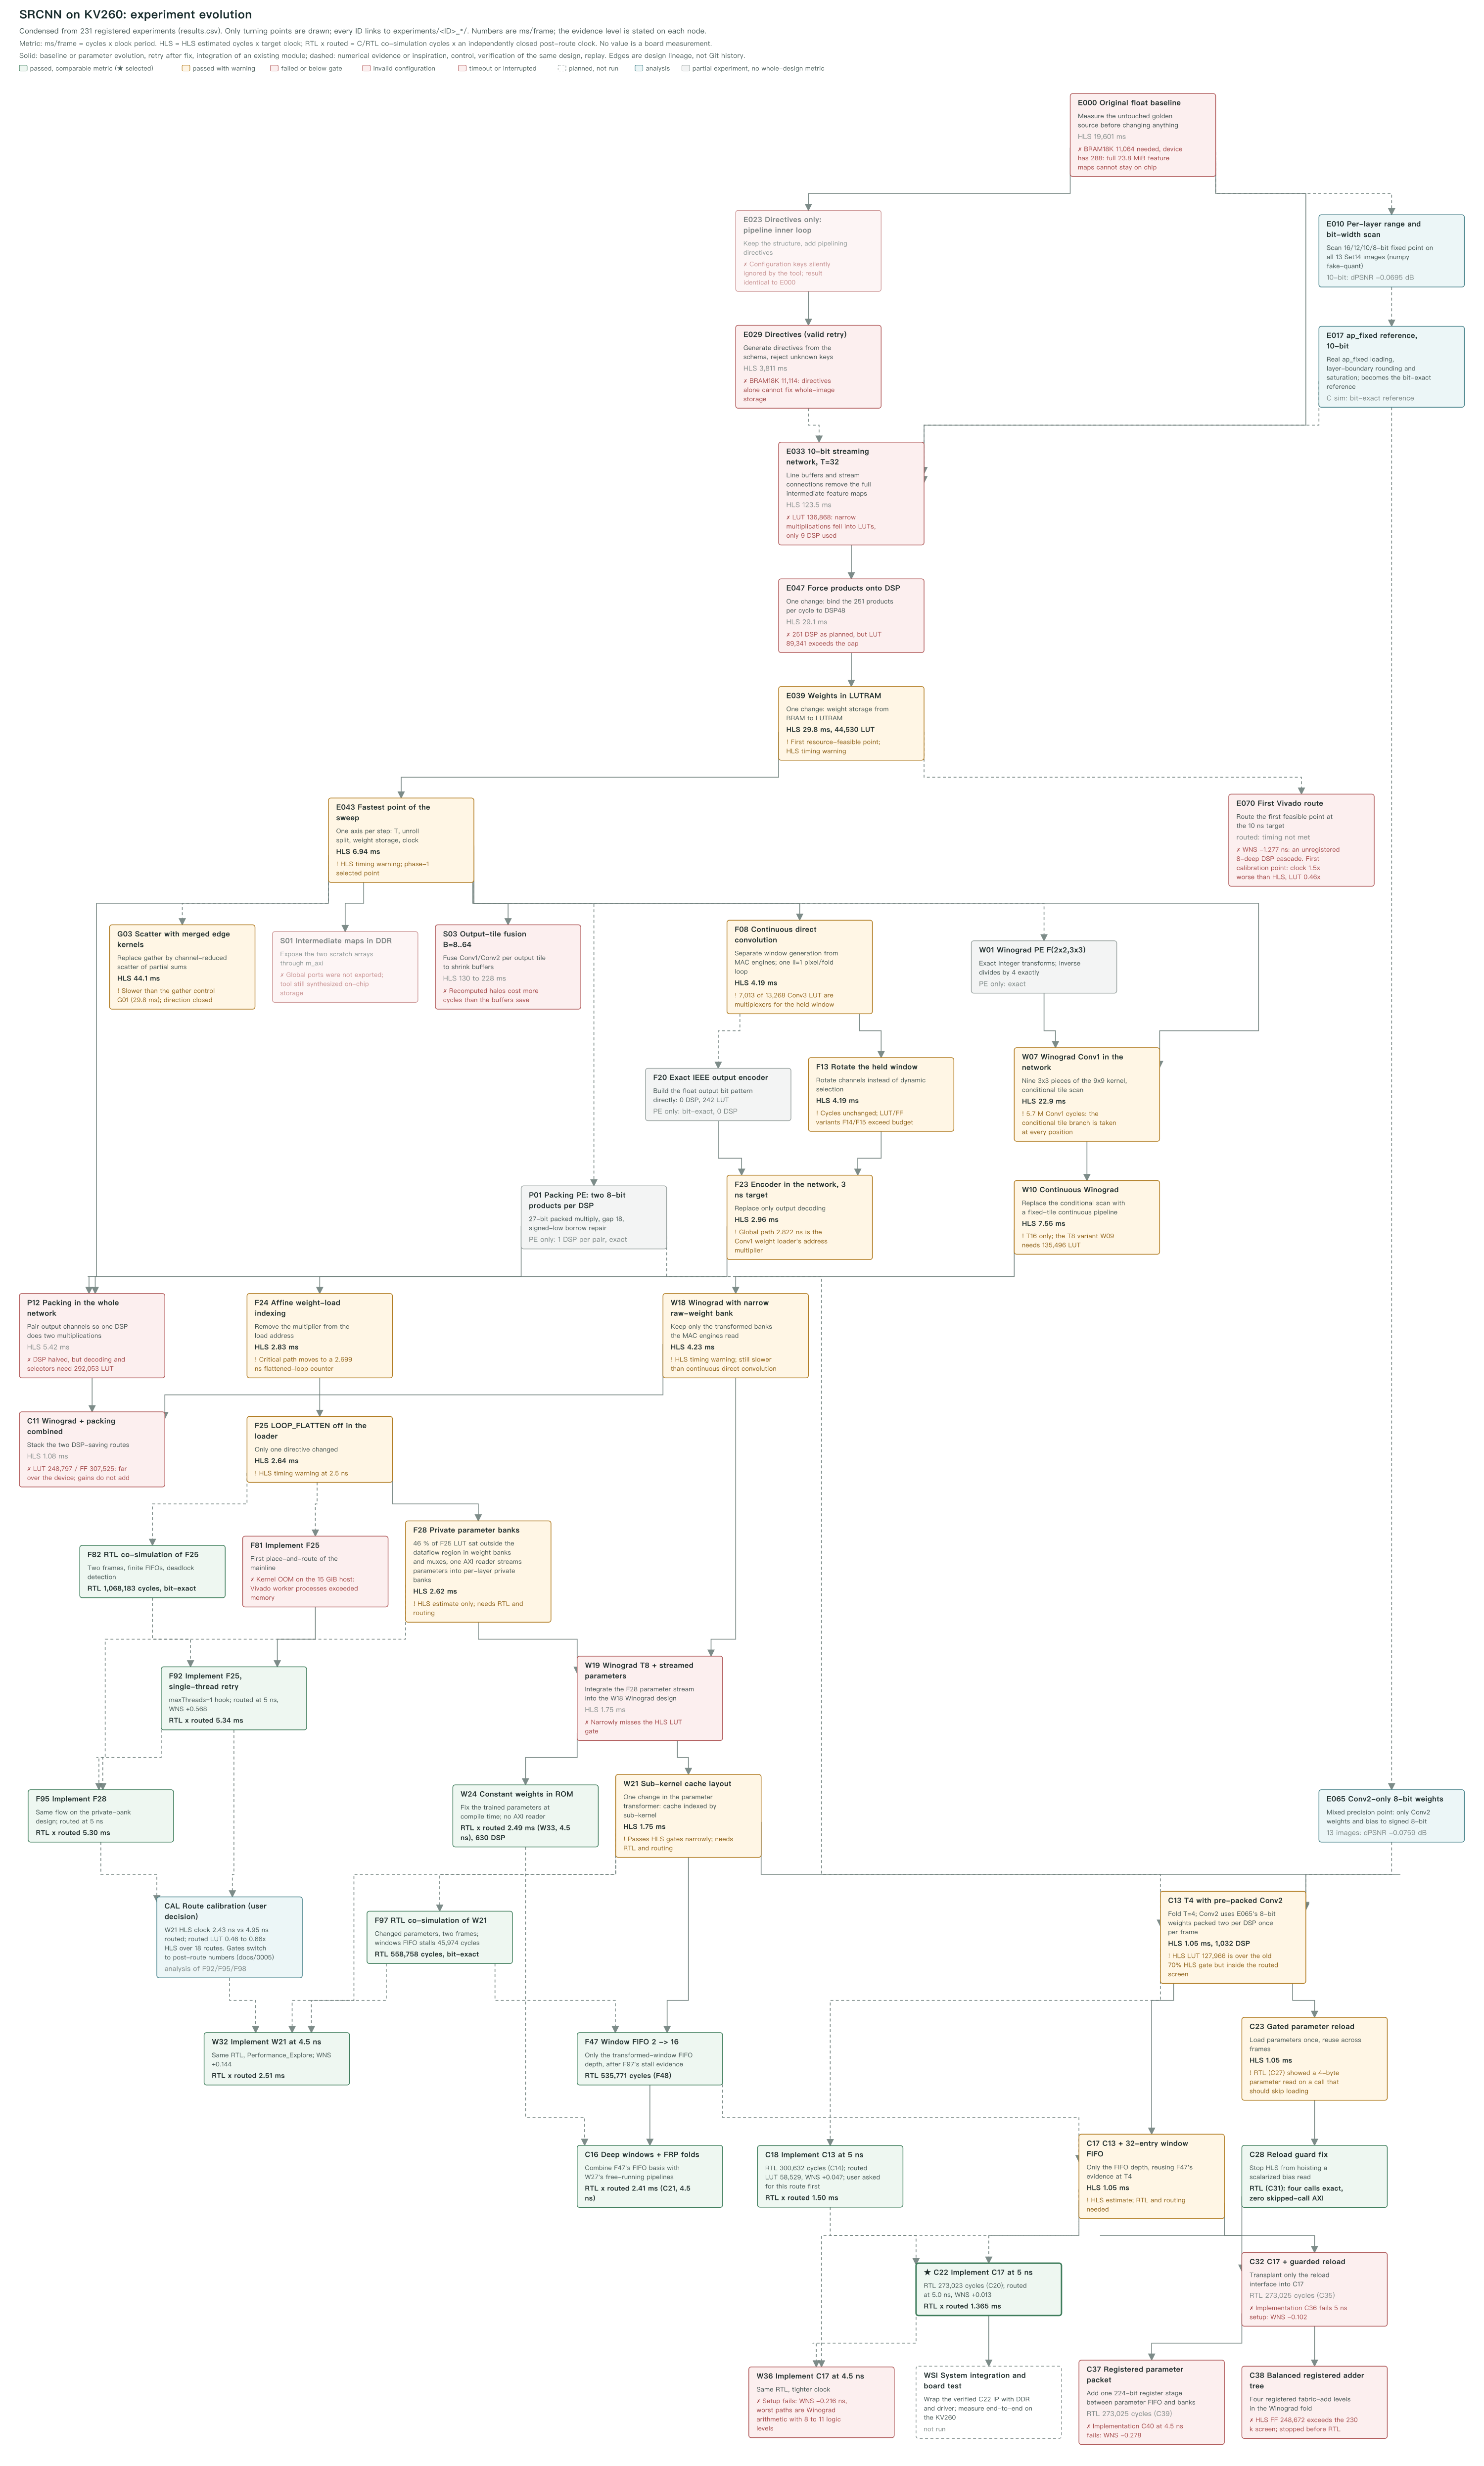
\includegraphics[width=\linewidth,height=0.95\figh,keepaspectratio]{figures/fig02-evolution-overview.png}
\caption{The search as a directed graph: 51 turning points out of 231 registered experiments. Solid edges are design lineage, dashed edges are evidence or verification; red nodes failed a gate, green nodes passed with a comparable number; the star marks the selected design C22.}
\label{fig:2}
\end{figure}

\subsection{Division of labour}\label{sec:3.5}

The agent did the mechanical and the clerical work: writing cards, copying and modifying designs, running the tools over SSH, parsing reports, updating the registry, drawing the graph, and drafting the interpretation of each run. It also proposed most of the individual experiments from the bottleneck evidence in the reports: the loader address multiplier in F23's timing report led to F24 and F25; the finding that 46 \% of F25's LUTs sat outside the dataflow region in weight banks and multiplexers led to the streamed-parameter designs F27 and F28; the FIFO stall profile of F97 led to F47.

We did the work that needs judgement about the goal rather than about the next step:

\begin{itemize}
\item writing and revising the high-level plans, and choosing which directions to pursue (Winograd and DSP packing were explored because the lectures covered them; the INT16 packing study P13 to P16 was requested by us);
\item changing the gates from HLS estimates to routed results on 2026-10-12 once the calibration data existed, and defining the 13 supplied images as the complete test set;
\item setting the host policy: how many jobs may run at once, the memory budget, enabling zram, and cleaning 55 GiB of old workspaces;
\item ordering priorities, for example asking for C18 to be routed before the planned T8 experiments, accepting F48 as the new T8 baseline, and declining a rescue re-route of C36 in favour of the verified C22;
\item reading every interpretation before the next plan was issued, roughly one review per 10 to 20 experiments.
\end{itemize}

Not every human decision was good. Our instruction to run two implementations at once caused the W23 out-of-memory failure; the one-heavy-job rule that replaced it came from the agent's measurement of the memory peaks.

\subsection{The directions we set}\label{sec:3.6}

In practice we set the following high-level directions, and the agent carried out the finer-grained implementation.

\begin{itemize}
\item \textbf{Fix the precision first, then work on the architecture.} The agent tried different precision requirements layer by layer, and in the first phase we settled on w10a10acc23 (10-bit weights, 10-bit activations, 23-bit accumulators), built a bit-exact \texttt{ap\_fixed} reference (E017, E019) and an exhaustive boundary check (E049). All two hundred or so later designs were required to match this reference bit for bit, so that every difference between experiments could be attributed to structure rather than to numerics. At the same time we explicitly rejected uniform INT8 (a 5.18 dB drop in mean PSNR on Set14) and admitted only 8-bit weights on Conv2 alone (E062, E065, a 0.0759 dB drop). This single exception later became the key to fitting the T4 design into the device.
\item \textbf{Abandon the directive-only route in the first phase.} E020 to E032 showed that the original code needs 11,064 BRAM18K no matter which pragmas are added. This negative result saved all later ``try one more pragma'' time and sent the search straight to a streaming architecture.
\item \textbf{Identify the weight-bank multiplexers as the real LUT bottleneck.} This was the most valuable single analysis of the whole trajectory (docs/0004 \S{}1.4). Breaking down the csynth report showed that 46 \% of the LUTs sat outside the dataflow region, in the multiplexers between the load loop and the engines across 324 to 648 LUTRAM banks. After F27 switched to streamed parameter loading, the out-of-region LUTs fell from 32 k to 3.2 k, and T8 became feasible.
\item \textbf{Judge feasibility by routed results, not HLS estimates.} This decision was made by us on 2026-10-12. The five calibration points available at the time all showed the HLS LUT estimate about 2$\times$ too high and the clock estimate about 2$\times$ too optimistic, and all 18 routed designs since have followed the same pattern. W21's HLS LUT count of 81,086 sat right at the threshold but routed to only 42.6 k; C13/C17 at 128 k HLS LUTs were ``infeasible'' under the old rule but routed to 59.5 k. Without this decision the T4 designs would never have been sent to place-and-route, and the 1.365 ms result would not exist. The companion decision was to stop tuning against the HLS clock estimate and look only at the routed critical path.
\item \textbf{Use Winograd only at T8/T4, not at T16.} At T16, W18 reduced the DSP count from 502 to 326 but left the cycle count unchanged, so there was no speed gain. Winograd only became useful once direct convolution at T8 needed 1,007 DSPs (81 \%) and Winograd brought that down to 648.
\item \textbf{Strict definitions of frame time and evidence level.} Only ``RTL cycles $\times$ closed clock'' counts; HLS estimates do not, and a period derived from negative WNS is treated as an estimate only. This prevented F25's 2.64 ms (at an estimated 2.5 ns) from being taken as a result; after routing it was 5.34 ms.
\item \textbf{Host resource management.} After three OOM kills we fell back to serial execution, then moved to ``one heavy job plus light jobs'' admitted under a memory budget, enabled zram, and cleaned 55 GiB of old workspaces. This is not a design decision, but it determined the experiment throughput.
\item \textbf{Three scope decisions.} The 13 supplied images are the complete test set; the interface may gain a \texttt{load\_params} switch; ROM parameter storage is exploratory only and does not enter the mainline. We made these three decisions on 12 and 13 October, and each one closed a bottomless pit.
\end{itemize}

\subsection{Limitations and lessons}\label{sec:3.7}

\begin{itemize}
\item \textbf{The method is expensive.} 231 experiments is far more than a human would run, and most of them are negative results or verification runs of the same design at another evidence level. The archive occupies several GB, the host ran continuously for three days, and the timeouts were 60 minutes for synthesis, 6 hours for co-simulation and 3 hours for implementation. The cost was worth paying only because each run is cheap to launch and the discipline makes negative results useful too.
\item \textbf{HLS estimates cannot be used for ranking.} For this design the HLS clock estimate is optimistic by 1.7 to 2$\times$ and the logic resource estimate pessimistic by about 2$\times$. Any search that ranks by HLS estimates would pick the wrong design. Routing is slow, so the compromise is to screen with HLS and rank only with routed numbers.
\item \textbf{The agent still needs a reviewer, and still makes mistakes.} The rules stop the agent from changing several things at once or overstating evidence, but they do not stop it from spending experiments on a direction that has stopped making sense; the review of the high-level plan is where that is corrected. The log also records clerical errors that the protocol caught after the fact: one experiment (W26) was launched before its design existed, one plan specified three co-simulation calls where four were needed, and a conditionally triggered implementation job was never started, leaving the host idle for several hours.
\item \textbf{The counts depend on the counting rules.} We count every registered run, including retries, controls and verification runs; there are 71 design directories, of which about 50 are distinct architectural points.
\item \textbf{No on-board feedback during the search.} All ranking during the search was based on RTL co-simulation and routed results; board integration was done only after the search ended. The gap between the on-board hardware time of 2.938 ms and the RTL $\times$ routed figure of 1.365 ms (166.665 MHz instead of 200 MHz, and single-beat AXI reads) was invisible at every evidence level available during the search, which shows that the top level of the evidence hierarchy cannot be skipped.
\end{itemize}

% Generated from the Notion page by tools/notion2tex.py (see report/README.md).
\section{Final Architecture}\label{sec:4}

The selected design is the one carried through all four verification steps: C17 (C simulation and HLS synthesis), C20 (C/RTL co-simulation) and C22 (Vivado place and route at 5 ns). Its source was produced by the agent over 200+ experiments. For reading, we had the agent rewrite it as a plain version with the macros substituted and the templates expanded, and re-ran C simulation and synthesis on both: the outputs are bit-identical and the synthesis results are the same.

The readable version is reproduced in Appendix~\ref{app:code-readable}; the original source is \path{designs/winograd_t4_windows32_v1/srcnn.cpp} in the project repository.

However, even so, we must mention that, for the agent optimization are extreme detailed, this chapter does not walk through the code. It explains the design one decision at a time: what constraint forced the decision, which experiment measured the alternatives, and what the chosen structure costs.

\subsection{Dataflow}\label{sec:4.1}

At the top level the design is organised by function, which gives a direct view of the dataflow.  The baseline was slow for a structural reason: inside each 16$\times$16 tile the three layers run one after another, every tile re-fetches a 28$\times$28 input window from DDR to produce 16$\times$16 outputs, the weights are reloaded over AXI on every call, and only 3.69 \% of the DSPs are ever busy. We wanted the opposite: keep everything the network produces on the chip, use no external scratch buffer at all (the one attempt with DDR scratch buffers, S01, was abandoned), and let the three layers work at the same time on different pixels. Task-level dataflow with \texttt{hls::stream} connections between the stages gives both at once.

The open question is how much to buffer between stages. Holding the full outputs of Conv1 and Conv2 (255$\times$255$\times$64 and 255$\times$255$\times$32 values) takes 23.81 MiB in float, while the device offers 5.1 Mb of BRAM and 18 Mb of URAM, about 2.9 MiB in total; even at 8 bits the two maps would not fit. So, neighbouring stages exchange single pixels (one pixel's channel vector), and only a stage that needs a spatial neighbourhood keeps a line buffer of a few rows, even more, every FIFO in the design has an explicitly chosen depth. Figure~\ref{fig:3} shows the resulting top-level structure.

\begin{figure}[!htbp]
\centering
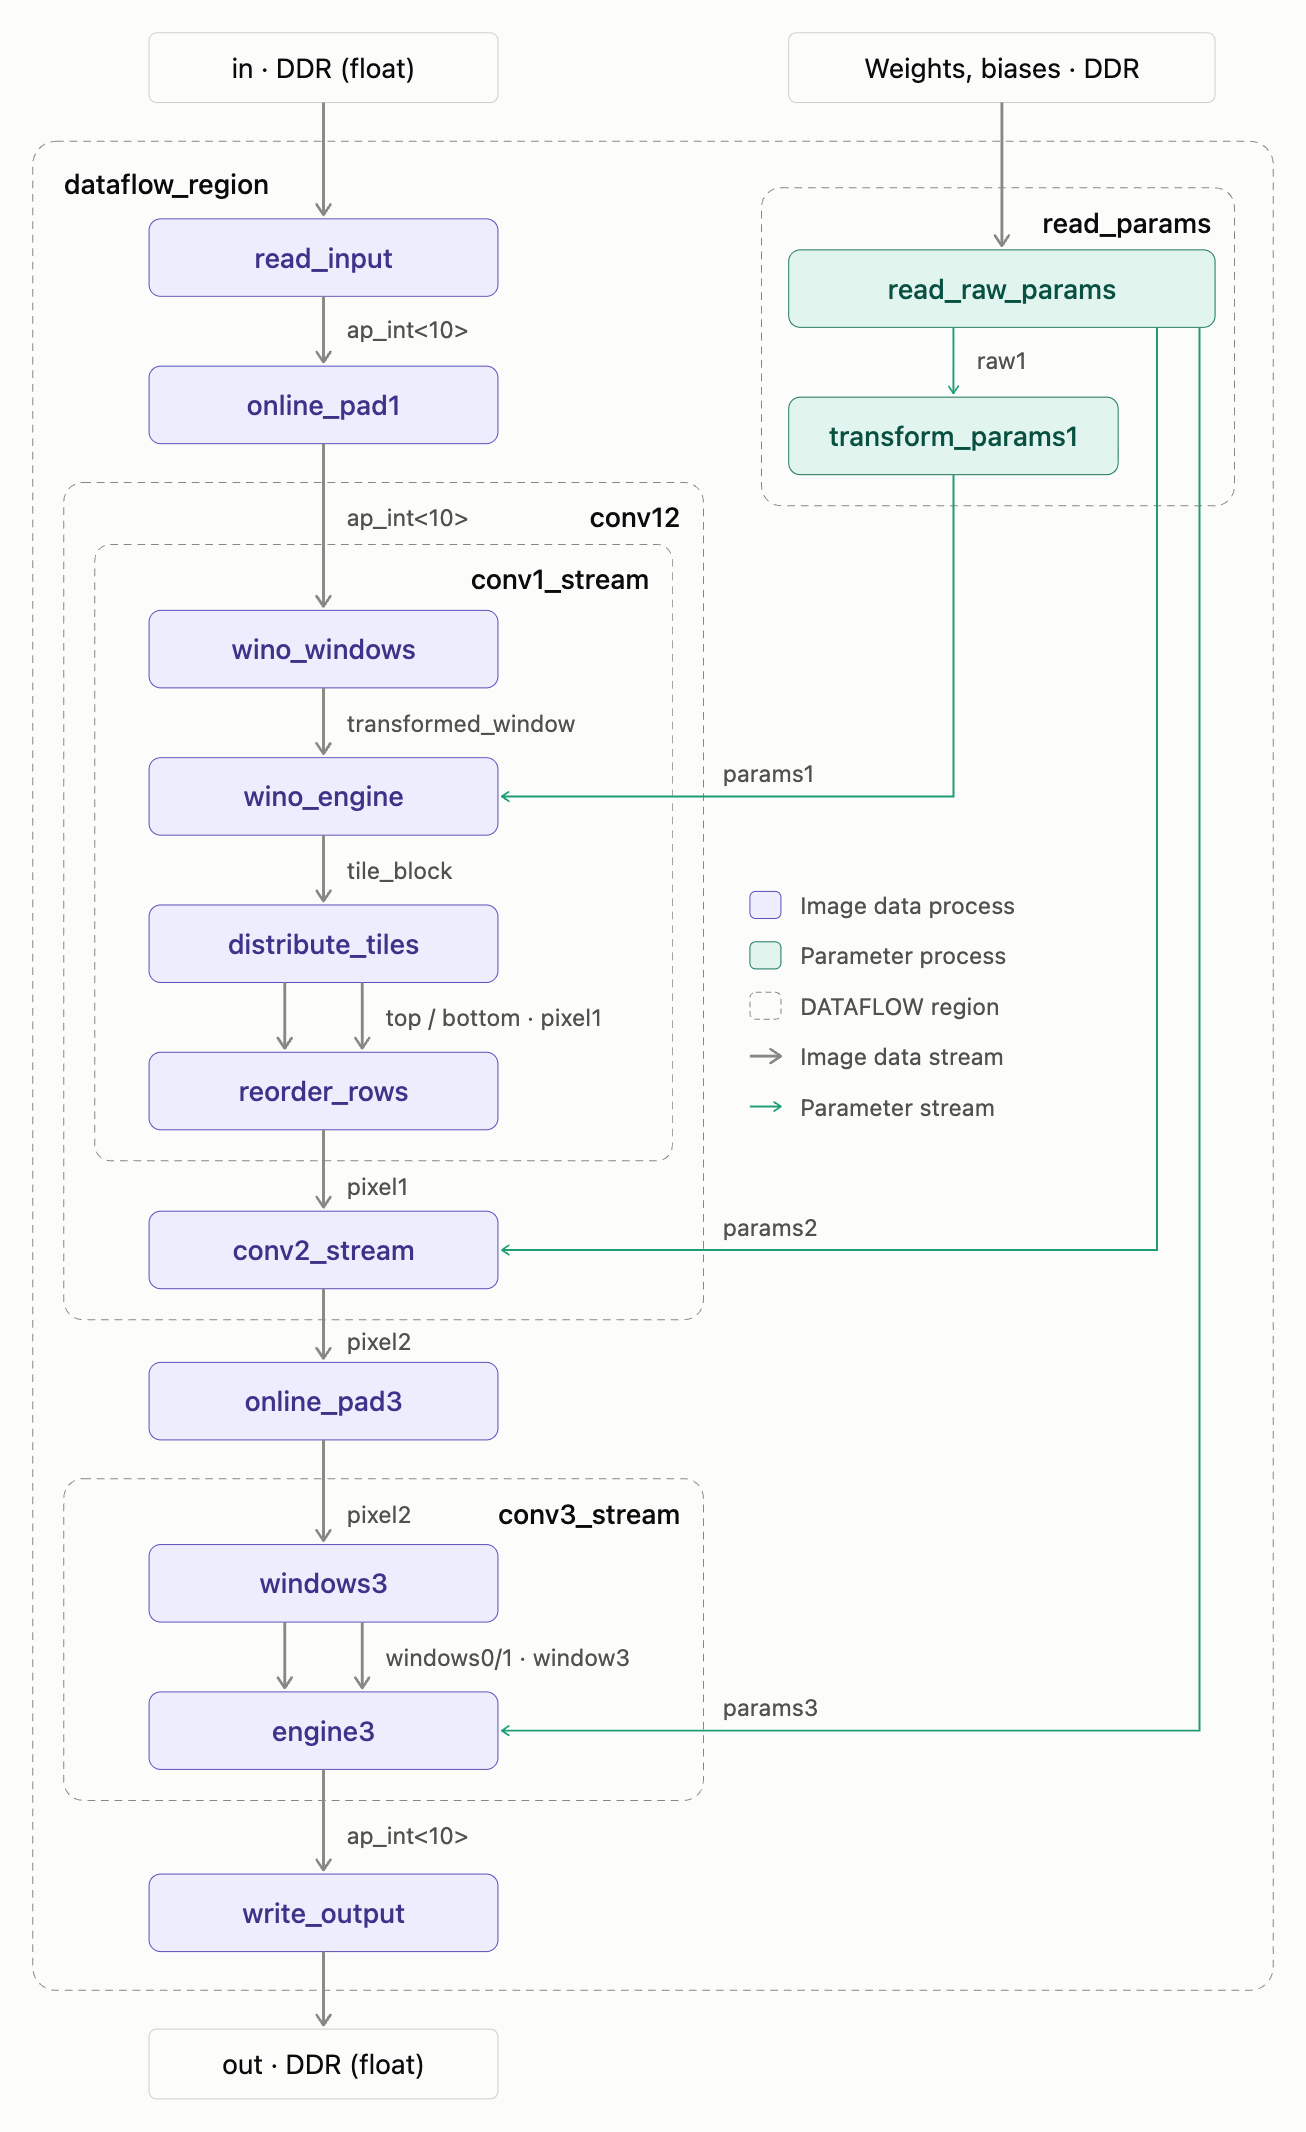
\includegraphics[width=0.72\linewidth,height=0.48\textheight,keepaspectratio]{figures/fig03-top-level-structure.png}
\caption{Top-level structure of the selected design: the dataflow region with its image-data processes (purple) and parameter processes (green), the nested DATAFLOW regions conv12, conv1\_stream and conv3\_stream, and the stream type passed between each pair of stages. Weights are read from DDR and transformed once per frame, then streamed to the three engines.}
\label{fig:3}
\end{figure}

\begin{table}[!htbp]
\centering
\scriptsize
\caption{Stages of the dataflow region of the selected design (C17), in data order: the element each stage passes on and its width, the FIFO depth, the on-chip memory it keeps (routed, C22), the loop trip count per frame from the source, and the active cycles and stall share measured in C/RTL co-simulation C20.}
\label{tab:3}
\begin{tabularx}{\linewidth}{lYR{0.9cm}R{1.3cm}YR{1.4cm}R{1.6cm}R{1.0cm}}
\toprule
Stage & Input $\rightarrow$ output element & Width (bits) & FIFO depth (out) & Internal memory & Iterations per frame (design) & Iterations per frame (C/RTL co-simulation) & Stall Percent \\
\midrule
\texttt{read\_input} & float from DDR $\rightarrow$ pixel \texttt{ap\_int<10>} & 10 & 512 & none & 65,025 & 78,653 & 66.9 \% \\
\texttt{online\_pad1} & pixel $\rightarrow$ pixel, 255\textsuperscript{2} $\rightarrow$ 264\textsuperscript{2} replicate-padded & 10 & 16 & 1 row, 255 $\times$ 10 b (1 BRAM18K) & 69,696 & 69,962 & 72.9 \% \\
\texttt{wino\_windows} & pixel $\rightarrow$ transformed window, 9 sub-blocks $\times$ 16 $\times$ \texttt{ap\_int<12>} & 1,728 & 32 (LUTRAM) & 9 rows $\times$ 264 $\times$ 10 b (9 BRAM18K) + 10$\times$10 window registers & 69,696 & 69,699 & 73.1 \% \\
\texttt{wino\_engine} & window $\rightarrow$ tile, 2$\times$2 pixels $\times$ 64 ch $\times$ 10 b & 2,560 & 2 (LUTRAM) & transformed weights 64 $\times$ 9 $\times$ 16 $\times$ 14 b = 129 kb (LUTRAM) & 262,144 & \textbf{262,924} & \textbf{2.5 \%} \\
\texttt{distribute\_tiles} & tile $\rightarrow$ 2 pixel streams (\texttt{top}, \texttt{bottom}), 64 ch $\times$ 10 b & 640 & 512 each (BRAM, 18 BRAM18K each) & none & 65,536 & 65,537 & 74.8 \% \\
\texttt{reorder\_rows} & 2 streams $\rightarrow$ raster-order pixel, 64 ch & 640 & 4 & none & 65,025 & 65,026 & 75.4 \% \\
\texttt{conv2\_stream} & 64-ch pixel $\rightarrow$ 32-ch pixel & 320 & 4 & packed weights 16 $\times$ 64 $\times$ 27 b = 27.6 kb (LUTRAM) & 260,100 & \textbf{262,275} & \textbf{3.2 \%} \\
\texttt{online\_pad3} & pixel $\rightarrow$ pixel, 255\textsuperscript{2} $\rightarrow$ 259\textsuperscript{2} padded & 320 & 16 & 1 row, 255 $\times$ 320 b (9 BRAM18K) & 67,081 & 67,347 & 75.3 \% \\
\texttt{windows3} & pixel $\rightarrow$ two half windows, 25 taps $\times$ 16 ch $\times$ 10 b each & 4,000 + 4,000 & 2 + 2 & 4 rows $\times$ 259 $\times$ 320 b (36 BRAM18K) + 5$\times$5$\times$32 window registers & 67,081 & 67,084 & 75.4 \% \\
\texttt{engine3} & two half windows $\rightarrow$ output pixel & 10 & 16 & weights 32 $\times$ 25 $\times$ 10 b = 8 kb (LUTRAM) & 260,100 & \textbf{260,977} & \textbf{4.4 \%} \\
\texttt{write\_output} & pixel $\rightarrow$ float to DDR & 32 & -- & none & 65,025 & 65,042 & 76.2 \% \\
\texttt{read\_params} $\rightarrow$ \texttt{transform\_params1} & 8,129 floats $\rightarrow$ three parameter streams & 224 / 10 / 10 & 4 / 16 / 16 & raw 9$\times$9 kernel registers & 8,129 + 640 & 10,487 / 7,234 & 0.2 \% / 1.4 \% \\
\bottomrule
\end{tabularx}
\end{table}

Table~\ref{tab:3} lists every process for one frame in the dataflow region with the shape and width of the element it passes on, the FIFO depth, the memory it keeps internally, and two numbers about time. \emph{Iterations per frame (design)} is the loop trip count read from the source: for a loop with II = 1 it is the number of cycles the stage needs when it is never blocked, so it is a lower bound, not a measurement. \emph{Iterations per frame (C/RTL co-simulation)} is measured after Vitis C/RTL co-simulation: from the latency of the process within one frame (\texttt{process\_latency\_avg\_cycles}, up to 273,052 cycles) we subtract \texttt{read\_stall\_cycles} and \texttt{write\_stall\_cycles}, which gives the number of cycles in which the stage was actually processing data. \emph{Stall Percent} is the share of the frame in which the process waited on a FIFO (\texttt{stall\_pct}).

Whether a dataflow pipeline is actually balanced can only be seen in C/RTL co-simulation, where every FIFO and process is instrumented. Figure~\ref{fig:4} shows the measured blocking of each FIFO over two RTL frames: the three engines (wino\_engine, conv2\_stream, engine3) wait less than 5 \% of the time, while every producer in front of them is write-blocked about 73 \% of the time and every consumer behind them is read-blocked about 75 \% of the time. This is the expected signature of a pipeline whose throughput is set by the compute engines rather than by the data movement. The inset records the one FIFO change that mattered: raising the window FIFO from depth 2 (C13/C14) to depth 32 (C17/C20) removed 58,166 read-block cycles from the Winograd fold loop and brought the frame from 300,632 to 273,023 cycles (1.503 ms to 1.365 ms at 5 ns).

\begin{figure}[!htbp]
\centering
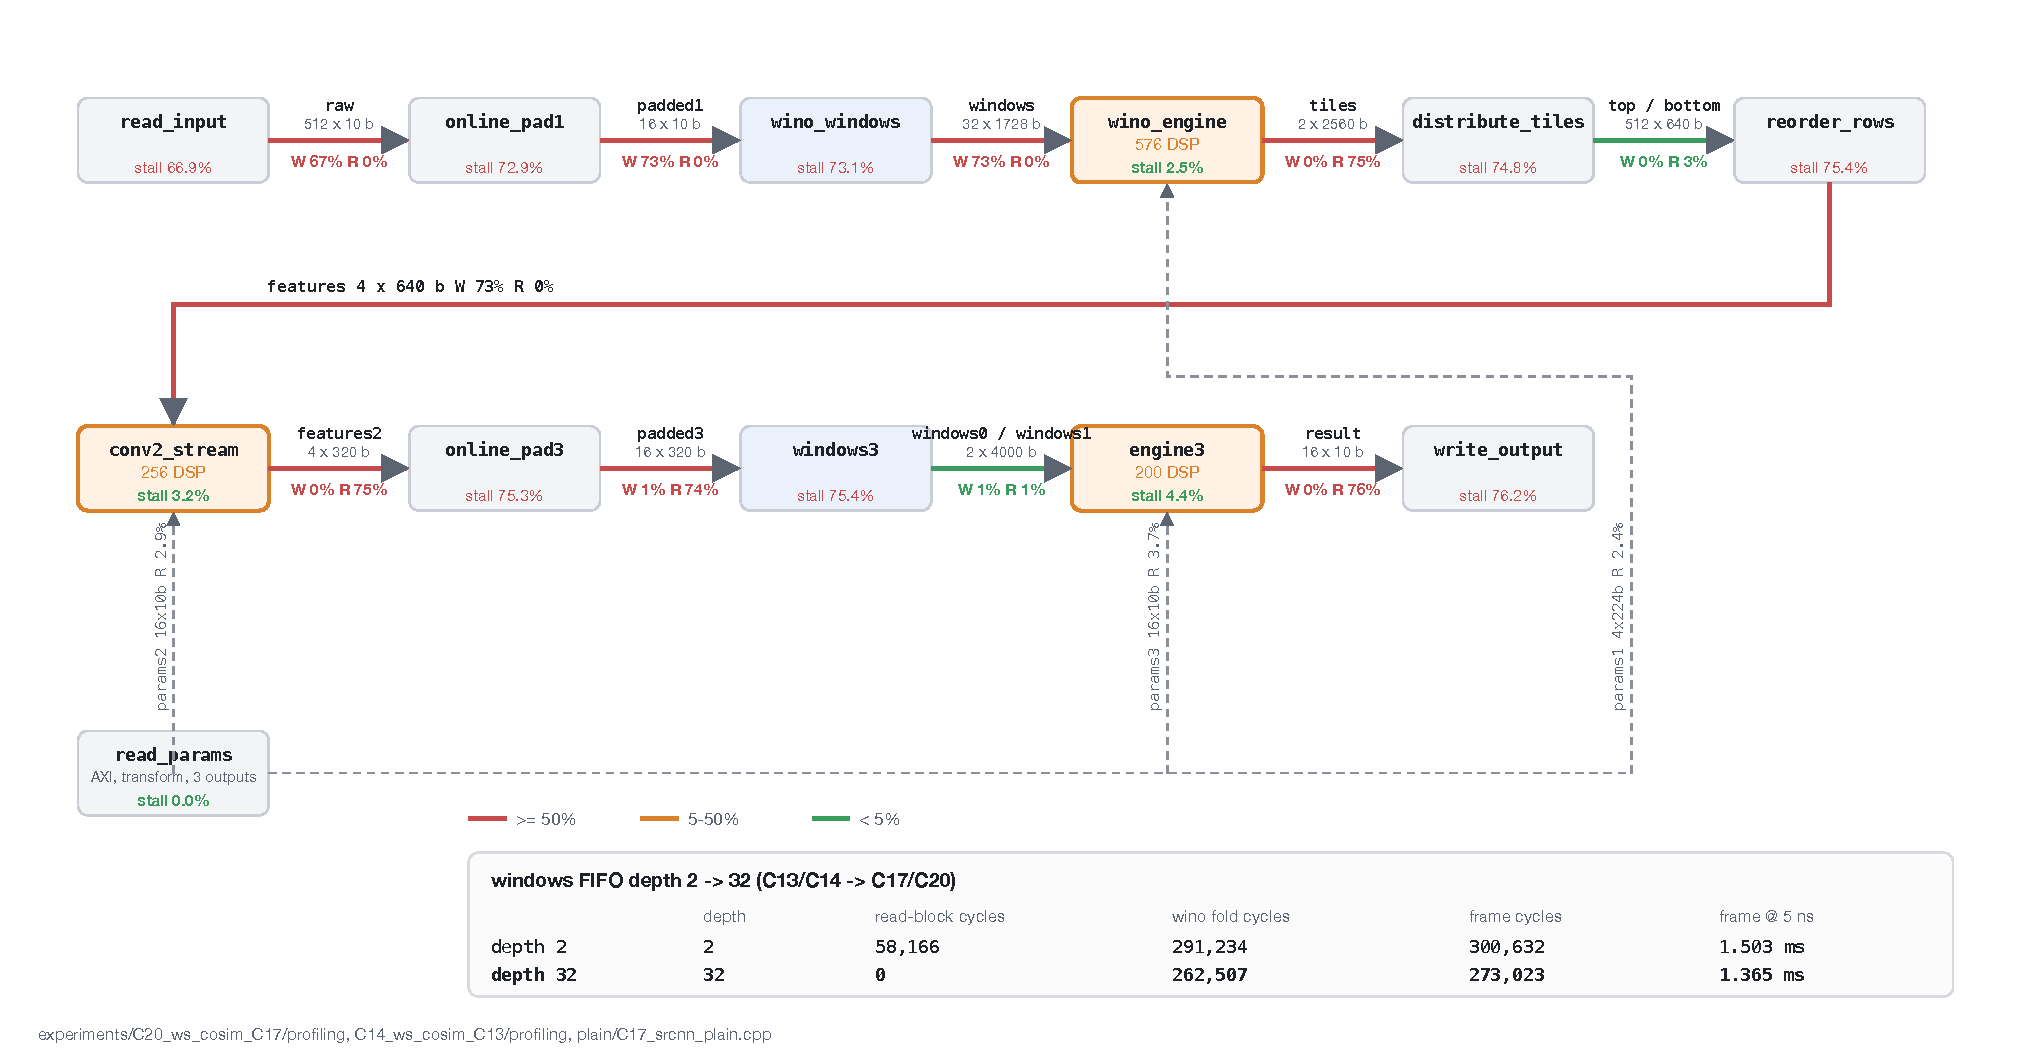
\includegraphics[width=\linewidth]{figures/fig04-dataflow-backpressure.pdf}
\caption{The dataflow region of the selected design: processes, FIFOs (depth $\times$ width in bits) and measured blocking from C/RTL co-simulation C20 over two frames. W / R is the share of cycles in which the FIFO blocked a write / a read; stall is the share of cycles in which the process waited. Inset: effect of the window FIFO depth, C14 (depth 2) against C20 (depth 32).}
\label{fig:4}
\end{figure}

\subsection{Resource allocation and optimisation for each layer}\label{sec:4.2}

MACs measure the amount of computation: to compute one output channel, every position in the K$\times$K window and every input channel is multiplied by a weight and accumulated, which is K$\times$K$\times$Cin operations; there are Cout output channels, so \textbf{MAC / output pixel = K $\times$ K $\times$ Cin $\times$ Cout.} Table~\ref{tab:4} gives the expected result for the three layers without any method magic.

\begin{table}[!htbp]
\centering
\footnotesize
\caption{Multiply-accumulate operations per output pixel for each layer of SRCNN and its share of the total.}
\label{tab:4}
\begin{tabular}{lllrr}
\toprule
Layer & Kernel & Channels & MAC / output pixel & Share \\
\midrule
conv1 & 9$\times$9 & 1$\rightarrow$64 & 5184 & 64.5\% \\
conv2 & 1$\times$1 & 64$\rightarrow$32 & 2048 & 25.5\% \\
conv3 & 5$\times$5 & 32$\rightarrow$1 & 800 & 10\% \\
\bottomrule
\end{tabular}
\end{table}

MACs decide resources. Building a multiplier out of logic is expensive on an FPGA, but the device provides DSP slices for exactly this, so we bind every multiplication to one DSP48E2 (one product per DSP per cycle; packing, which fits two, is introduced later). We then introduce the fold factor T: the number of clock cycles an engine spends on one output pixel. A layer with MAC multiplications per pixel takes T cycles per pixel, but needs only MAC/T multipliers, so T trades time for DSPs. The device has 1,248 DSP48E2 slices, so the task is to choose the smallest T whose DSP demand still fits, which is also the T that uses the device most fully.

At T = 4, direct conv1 alone needs 1,296 DSPs, more than the device has, and even Winograd conv1 with direct conv2 still needs 1,288. T = 4 becomes feasible only when both techniques are used together: Winograd on conv1 and packing on conv2, with conv3 small enough to stay direct (1,032 DSPs). T = 8 and T = 16 fit easily but double and quadruple the frame time, and T = 2 is out of reach with any combination. So T = 4 is the fastest fold that fits, and it is the row of Table~\ref{tab:5} where the two reductions are necessary rather than merely helpful.

\begin{table}[!htbp]
\centering
\footnotesize
\caption{DSPs needed per layer as a function of the fold T (cycles per output pixel), for the direct algorithm and for the selected reductions. Products per pixel: conv1 direct 5,184, conv1 Winograd 2,304; conv2 direct 2,048, conv2 packed 1,024 DSP-equivalents; conv3 800. The device limit is 1,248. The last column is the DSP count measured in synthesis for the experiments that implemented that row.}
\label{tab:5}
\begin{tabularx}{\linewidth}{cC{1.15cm}C{1.25cm}C{1.15cm}C{1.25cm}C{1.15cm}C{1.3cm}C{1.4cm}C{1.5cm}Y}
\toprule
T & conv1 direct & conv1 Winograd & conv2 direct & conv2 packed & conv3 direct & Total, all direct & Total, Winograd only & Total, Winograd + packing & Measured \\
\midrule
1 & 5,184 & 2,304 & 2,048 & 1,024 & 800 & 8,032 & 5,152 & 4,128 & -- \\
2 & 2,592 & 1,152 & 1,024 & 512 & 400 & 4,016 & 2,576 & 2,064 & -- \\
\textbf{4} & 1,296 & 576 & 512 & 256 & 200 & \textbf{2,008} & \textbf{1,288} & \textbf{1,032} & C13/C17: 1,032 \\
8 & 648 & 288 & 256 & 128 & 100 & 1,004 & 644 & 516 & F29/F30: 1,004; W21: 644; C10: 520 \\
16 & 324 & 144 & 128 & 64 & 50 & 502 & 326 & 258 & W18: 326 \\
\bottomrule
\end{tabularx}
\end{table}

The outcome of this allocation is shown in Table~\ref{tab:6}. After Winograd the three layers need 151 M, 133 M and 52 M multiplications per frame; with 576, 256 (each computing two products) and 200 DSPs, every layer needs 4 cycles per output pixel, a design bound of 4 $\times$ 255 $\times$ 255 = 260,100 cycles per frame. The C/RTL co-simulation C20 measured the three fold loops at 262,507, 260,877 and 261,885 cycles, within 1 \% of the bound and of each other. Because the stages run concurrently in a dataflow pipeline, the frame time is set by the slowest stage; the measurement confirms that no layer waits for another.

\begin{table}[!htbp]
\centering
\footnotesize
\caption{Fold-loop cycles per frame for the three engines: the design bound (loop trip count from the source) against the latency measured in C/RTL co-simulation C20. conv1 is bounded at 262,144 rather than 260,100 because its 2$\times$2 tiles cover a 256$\times$256 padded image.}
\label{tab:6}
\begin{tabular}{lrrr}
\toprule
layer & theory lower bound & C/RTL co-simulation & extra \\
\midrule
conv1(with edge padding) & 262,144 & 262,507 & +0.14 \% \\
conv2 & 260,100 & 260,877 & +0.30 \% \\
conv3 & 260,100 & 261,885 & +0.69 \% \\
\bottomrule
\end{tabular}
\end{table}

\subsection{Conv1: Winograd on nine 3$\times$3 sub-kernels}\label{sec:4.3}

\subsubsection{Principle}\label{sec:4.3.1}

Multiplication is expensive on an FPGA because it consumes DSPs, which are scarce; addition goes to LUTs, which are far cheaper. In the first layer, each output pixel needs the 9$\times$9 window of input pixels around it, for each of 64 output channels. But the windows of neighbouring output pixels obviously overlap, and the direct method still recomputes everything for each of them.

The smallest case, F(2,3), computes two outputs of a 3-tap filter from four inputs with 4 multiplications instead of 6:

\begin{lstlisting}[language={}]
# directly
y0 = d0·g0 + d1·g1 + d2·g2
y1 = d1·g0 + d2·g1 + d3·g2

# winograd: 
m1 = (d0 - d2) · g0
m2 = (d1 + d2) · (g0 + g1 + g2)/2
m3 = (d2 - d1) · (g0 - g1 + g2)/2
m4 = (d1 - d3) · g2

y0 = m1 + m2 + m3
y1 = m2 - m3 - m4
\end{lstlisting}

\subsubsection{Winograd on FPGA}\label{sec:4.3.2}

A very important property was utilized, which is that, for \textbf{multiplications or divisions that ever appear are $\times$2, $\times$\textonehalf{} and $\times$4, on FPGA those are binary shifts, which are fast and essentially free.}

The weight-side terms (g0 + g1 + g2)/2 are computed once when the weights are loaded; the input-side terms d0 $-$ d2 and the output sums are additions, which go to LUTs. The 2-D form F(2$\times$2, 3$\times$3) applies the same transforms along rows and columns: a 4$\times$4 input tile is transformed (B\textsuperscript{T} d B), multiplied element-wise by the transformed 3$\times$3 kernel (G g G\textsuperscript{T}), and the 4$\times$4 product is transformed back (A\textsuperscript{T} m A) to a 2$\times$2 output tile. That is 16 multiplications instead of 36 per 2$\times$2 tile, 2.25$\times$ fewer.

In integer arithmetic the \textonehalf{} in G is a division, which drops the lowest bit, and the Winograd result would no longer match the direct convolution. The fix is to use 2G instead of G, so the matrix becomes integer. In two dimensions the weight transform is U = (2G)$\cdot$g$\cdot$(2G)\textsuperscript{T}, which is the true U scaled by 4. Every later operation, the input transform, the element-wise products, the sum over the nine sub-blocks and the output transform, is then an integer add or multiply with no rounding, so the number that comes out is exactly 4 times the direct integer convolution result, its two lowest bits are always zero, and a right shift by 2 restores it bit for bit.

The transforms do widen the operands. Each transformed input value is a sum or difference of up to four pixels, so 10 bits become 12; each transformed weight is a sum of up to nine weights scaled by 2, so 10 bits become 14. The DSP48E2 multiplier is 27 $\times$ 18 bits, so a 12 $\times$ 14-bit product fits in one DSP, and each of the 16 products per tile costs exactly one DSP. The same widths are also why conv1 cannot use the two-products-per-DSP packing of conv2: two 14-bit weights at the 18-bit spacing that packing needs would occupy 32 bits, more than the 27-bit port, and the low-field product 12 $\times$ 14 = 26 bits would overflow the 18-bit field anyway. Winograd and packing are therefore not combined on the same layer; conv1 gets Winograd, conv2 gets packing.

\subsubsection{Why nine 3$\times$3 sub-kernels rather than a bigger tile.}\label{sec:4.3.3}

The 9$\times$9 kernel is cut into a 3$\times$3 grid of 3$\times$3 sub-kernels (the \texttt{group} index in the code). A 9-tap convolution is the sum of three 3-tap convolutions applied to the input at offsets 0, 3 and 6, and in two dimensions the 9$\times$9 convolution is the sum of nine 3$\times$3 convolutions at offsets (3a, 3b); nothing is approximated by the split. Each of the nine 3$\times$3 convolutions is then computed with Winograd F(2$\times$2, 3$\times$3), which produces a 2$\times$2 block of outputs from a 4$\times$4 block of inputs with 16 multiplications instead of 36. The 2$\times$2 output tile therefore needs a 10$\times$10 input window (2 + 9 $-$ 1 in each direction), and sub-kernel (a, b) reads the 4$\times$4 sub-block of that window starting at row 3a and column 3b; neighbouring sub-blocks share one row or column because a 3$\times$3 kernel on a 2$\times$2 tile needs 4$\times$4 input. The nine 4$\times$4 products are added in the transformed domain and the output transform runs once on the sum, which is valid because the transform is linear. One tile costs 9 $\times$ 16 = 144 multiplications for 4 pixels, 36 per pixel against 81 direct, a 2.25$\times$ reduction.

Working in 2$\times$2 tiles has a price downstream. The engine emits one tile every 16 cycles, but conv2 consumes pixels in raster order, so two processes after the engine (\texttt{distribute\_tiles}, \texttt{reorder\_rows}) split each tile into its upper and lower pixel pair and interleave even and odd rows back into scan order. Holding the odd rows until the even rows have gone out takes two 512-deep, 640-bit FIFOs, 36 BRAM18K, which is the largest memory cost of this layer, larger than the 9-row line buffer itself (9 BRAM18K). The padded image is also made 264$\times$264 instead of 263$\times$263 so that 128 $\times$ 128 tiles cover it exactly; the extra output row and column are discarded.

The tile size is a free parameter of Winograd: F(m, 3) computes m outputs per 1-D tile for any m, and m = 255 would process a whole image row at once. Larger tiles save more multiplications (per output pixel, ((m + 2)/m)\textsuperscript{2} against 9: 4 for m = 2, 2.25 for m = 4, approaching 1), so the question is why m = 2 is used. The answer is the transform constants, and multiplications cost . F(m, r) is built from polynomial interpolation at m + r $-$ 1 points; for m = 2 those are 0, 1, $-$1 and $\infty$, and the resulting matrices contain only 0, $\pm$1 and \textonehalf{}, which is why multiplying G by 2 makes everything integer and a 2-bit shift restores the result exactly. For m = 4 the interpolation needs six points (adding $\pm$2), and G contains 1/4, 1/6, 1/12 and 1/24: the smallest integer scaling is 24 per dimension, the result comes out 576 times too large, and dividing by 576 is no longer a shift. Besides, the transformed window is streamed as one element every T cycles, and its width is 9 sub-blocks $\times$ (m + 2)\textsuperscript{2} values $\times$ the transformed width: 1,728 bits for m = 2, but about 5,500 bits for m = 4 (36 values per sub-block, 17-bit operands), above the 4,096-bit aggregate stream limit of Vitis HLS that C09 ran into. Finally, a smaller conv1 would not shorten the frame on its own: with m = 4 conv1 needs 324 DSPs instead of 576 at T = 4, but the frame time is set by T, and moving the whole network to T = 2 fails on conv2 and conv3 regardless. Table~\ref{tab:7} collects the options. F(2$\times$2, 3$\times$3) is the only tile that is exact with shifts, nine of them cover the 9$\times$9 kernel without padding, and it is the one that was built and measured.

\begin{table}[!htbp]
\centering
\footnotesize
\caption{Options for conv1 at T = 4. Only the first two were synthesised; the F(4$\times$4, 3$\times$3) row is a paper estimate and was not pursued for the reasons in the text.}
\label{tab:7}
\begin{tabularx}{\linewidth}{YR{1.6cm}R{1.5cm}L{2.2cm}L{2.6cm}L{2.0cm}}
\toprule
Algorithm & Products per output pixel (64 ch) & DSPs at T = 4 & Transform constants & Exact with integer shifts & Window stream width \\
\midrule
Direct 9$\times$9 & 5,184 & 1,296 (> 1,248) & -- & yes & 10 b pixel \\
Nine 3$\times$3 sub-kernels, F(2$\times$2, 3$\times$3) \textbf{(selected)} & 2,304 & 576 & 1, \textonehalf{} & yes (G $\times$ 2, result >> 2) & 1,728 b \\
Nine 3$\times$3 sub-kernels, F(4$\times$4, 3$\times$3) & 1,296 & 324 & 1, \textonehalf{}, \textonequarter{}, 1/6, 1/12, 1/24 & no (scale 24\textsuperscript{2}, division by 9 remains) & $\approx$ 5,500 b (> 4,096 limit) \\
\bottomrule
\end{tabularx}
\end{table}

\textbf{Pipeline.} The layer is four processes (Table~\ref{tab:3}). \texttt{wino\_windows} slides a 10$\times$10 window over the padded 264$\times$264 image with a 9-row line buffer, and every second row and column emits the nine transformed 4$\times$4 sub-blocks as one 1,728-bit element. \texttt{wino\_engine} spends 16 cycles per window: in each cycle 4 output channels (4 lanes $\times$ 9 sub-blocks $\times$ 16 taps = 576 DSP products) are accumulated in the transformed domain, output-transformed, shifted, biased, and passed through ReLU and the round-to-10-bit quantiser; the 64 channels of the 2$\times$2 tile are collected in a shift register and written after cycle 15. \texttt{distribute\_tiles} and \texttt{reorder\_rows} turn tiles back into raster order and drop the extra row and column that the padding added so that 2$\times$2 tiles cover 255 pixels.

\subsection{conv2: two output channels per DSP}\label{sec:4.4}

\textbf{Budget.} conv2 is 25.5 \% of the MACs: 64 input channels $\times$ 32 output channels = 2,048 products per pixel, 512 DSPs at T = 4. The layer has 32 output channels but a 1$\times$1 kernel, so there is no spatial overlap to exploit and Winograd does not apply. Its DSP count still has to come down: with Winograd on conv1 and direct conv2 the network needs 1,288 DSPs, more than the 1,248 on the device.

\begin{figure}[!htbp]
\centering
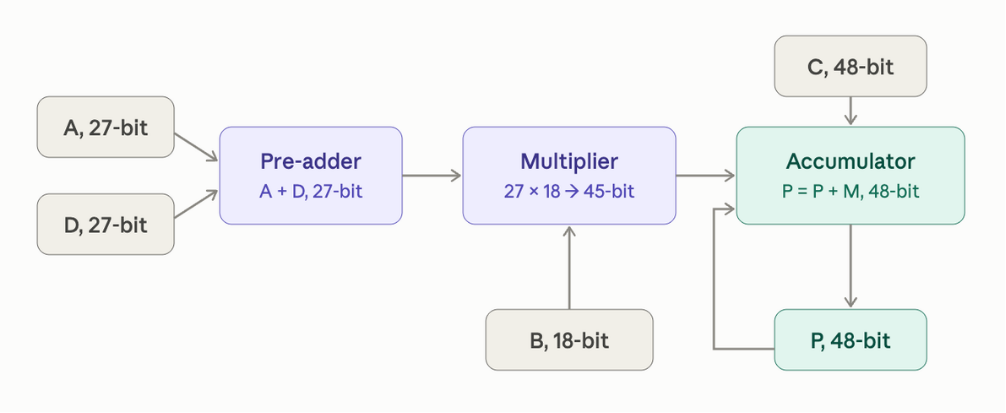
\includegraphics[width=0.8\figw]{figures/fig05-dsp48e2.png}
\caption{The DSP48E2 slice used for every multiplication in the design: a 27-bit pre-adder, a 27 $\times$ 18-bit signed multiplier and a 48-bit accumulator. conv2 packing places two 8-bit weights in the 27-bit A operand and the activation in the 18-bit B operand, so one multiplier yields two products; the pre-adder and accumulator are not used, because the sums are formed in fabric adder trees.}
\label{fig:5}
\end{figure}

\textbf{Principle.} A DSP48E2 multiplies a 27-bit by an 18-bit signed operand. The conv2 operands are a 10-bit activation and an 8-bit weight, so most of the 27-bit port is unused. Two weights for two output channels, w0 and w1, which share the same input activation x, are placed in one 27-bit word with a gap of 18 bits, \texttt{packed = w0 $\times$ 2\^{}18 + w1}. The single product is then

\begin{equation}
\text{packed} \times x = (w_0 \times x) \times 2^{18} + (w_1 \times x)
\end{equation}

A 10-bit activation times an 8-bit weight needs at most 17 bits plus a sign, so w1 $\times$ x stays inside the low 18 bits and never reaches the field of the second weight at bit 18 and above. Signs need no special arithmetic either: a negative w1 $\times$ x simply appears in the low field in two's complement, and because the packed word was formed as the integer w0 $\times$ 2\^{}18 + w1 (a negative w1 has already borrowed one from the w0 field), the DSP performs an ordinary integer multiplication. The only correction is at readout: when the low field is negative (bit 17 set) the high field reads w0 $\times$ x $-$ 1, and the engine adds the 1 back.

The packing itself is done once per frame when the weights are loaded (2,192 cycles), so no packing arithmetic runs per pixel; what remains per pixel is the borrow repair and the adder trees.

Why 8-bit weights are acceptable here is answered by the precision scan in Table~\ref{tab:8}. The smallest uniform precision that passes the $-$0.1 dB gate is 10-bit weights with 10-bit activations; uniform 8-bit weights lose about 5 dB. Quantizing only conv2 to 8-bit weights, however, passes: it costs 0.006 dB more than the uniform 10-bit point. There was also a way to pack without giving up 10-bit weights: the agent first split each weight into an 8-bit low part and a residual that is corrected after the multiplication (P07: exact, 1 DSP per pair, but 454 LUTs instead of 132). Applied to the whole network that costs 292,000 LUTs at T = 4 (P12), 2.5$\times$ the device, so conv2 carries 8-bit weights and a 21-bit accumulator while conv1 and conv3 keep 10-bit weights and are not packed.

\begin{table}[!htbp]
\centering
\footnotesize
\caption{Mean PSNR change of the fixed-point network against the float golden output over 13 images, from the precision scan E010 and the mixed-precision runs E062/E065. The gate for a design to be ranked was $-$0.1 dB.}
\label{tab:8}
\begin{tabular}{lrrll}
\toprule
Weights & Activations & $\Delta$PSNR (dB) & Worst image (dB) & Passes $-$0.1 dB gate \\
\midrule
16 & 10 & $-$0.046 & $-$0.171 & yes \\
10 & 10 & $-$0.070 & $-$0.226 & yes \\
10 & 8 & $-$0.645 & $-$1.958 & no \\
8 & 10 & $-$4.955 & $-$11.84 & no \\
8 & 8 & $-$5.180 & $-$12.14 & no \\
\textbf{10, conv2 only 8 (selected)} & \textbf{10} & \textbf{$-$0.076} & \textbf{$-$0.268 (foreman)} & \textbf{yes} \\
\bottomrule
\end{tabular}
\end{table}

\textbf{Pipeline.} \texttt{conv2\_stream} is one II = 1 loop that spends 4 cycles per pixel. In each cycle four lanes each take one channel pair: 64 packed multiplies, 64 borrow repairs, two 64-input adder trees (6 fabric levels, one register each), bias, truncation to 21 bits, ReLU and rounding to 10 bits; the 8 channels per cycle are collected in a shift register and the 32-channel pixel is written after cycle 3. Per cycle that is 256 DSPs producing 512 products. The widths along the path are: 37-bit product, 23-bit sums, 21-bit accumulator before ReLU, 10-bit output with 7 fraction bits. The 21-bit truncation relies on the sum range, which the C simulation checks with an assertion over the test set.

\textbf{Cost.} HLS estimate: 256 DSPs, 37,074 LUTs, 80,091 FFs. Routed (C22): 256 DSPs, 16,009 LUTs, 17,759 FFs, no BRAM. The 2.3$\times$ LUT and 4.5$\times$ FF difference between estimate and routed result is the largest of the three layers and comes from the register-heavy adder trees that Vivado retimes.

\subsection{conv3: direct 5$\times$5 convolution, folded over four cycles}\label{sec:4.5}

\textbf{Budget.} conv3 is 10 \% of the MACs: 25 taps $\times$ 32 input channels = 800 products per output pixel, 200 DSPs at T = 4. Since the main step that limits the speed is not conv3, therefore, as long as conv3 can complete the task within T = 4 using limited resources, it will be sufficient.

\textbf{Principle.} The layer is a classic streaming convolution: a line buffer plus a sliding window. \texttt{windows3} keeps the last four rows of the padded 259$\times$259 feature map, 32 channels of 10 bits each, in BRAM (4 $\times$ 259 $\times$ 320 bits = 36 BRAM18K), and a 5$\times$5$\times$32 window in registers. Each incoming pixel shifts the window one column: the new column is the four stored rows plus the new pixel, and the line buffer shifts up one row at the same address. From the fifth row and column on, every pixel yields a complete window, so the stage emits 65,025 windows for 67,081 input pixels. The window is 8,000 bits and goes out as two 4,000-bit halves (channels 0 to 15 and 16 to 31) because of the 4,096-bit stream limit noted in the dataflow section.

\texttt{engine3} folds the 800 products over 4 cycles: in cycle k it multiplies input channels 8k to 8k+7 by all 25 taps (200 DSPs, 10 $\times$ 10 $\rightarrow$ 20 bits), zero-pads the 200 products to 256 and adds them in an 8-level fabric adder tree with one register per level, then adds the partial to a 23-bit running sum that starts from the bias in cycle 0. After cycle 3 the sum is rounded half to even to 10 bits with saturation and written out. There is no ReLU; the 10-bit integer is decoded to a float exactly by assembling the IEEE fields rather than by a float-conversion core. The pipeline depth of 13 cycles is mostly the adder tree; at II = 1 this depth is paid once per frame, not per pixel.

\begin{figure}[!htbp]
\centering
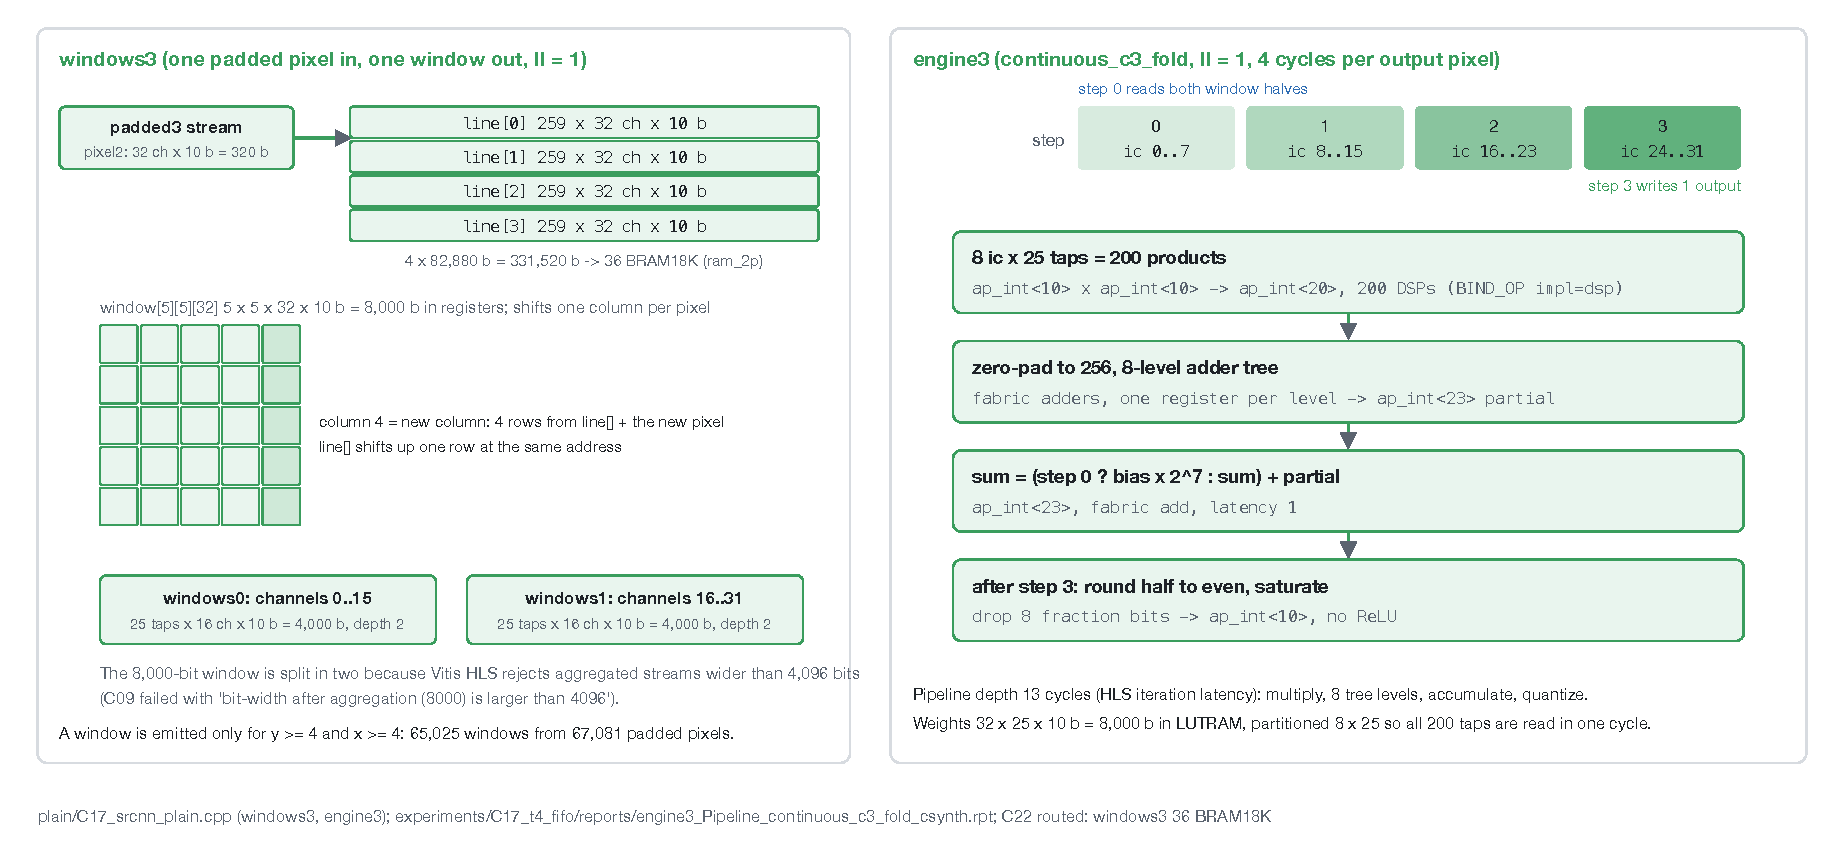
\includegraphics[width=\linewidth]{figures/fig06-conv3-window-engine.pdf}
\caption{conv3: window generation and folded engine. Left: four line-buffer rows and the 5$\times$5$\times$32 register window; the window leaves as two 4,000-bit halves. Right: the four-cycle fold, 200 DSP products and a 256-input adder tree per cycle, accumulated into a 23-bit sum.}
\label{fig:6}
\end{figure}

\textbf{Why it stays direct.} The alternatives were measured and rejected. A scatter formulation, which stores five rows of partial sums instead of four rows of input and adds each incoming pixel into the 25 outputs it affects, cuts conv3 BRAM from 36 to 5 blocks but costs 34 \% to 56 \% more cycles (G01 to G03, controlled comparison at T = 32), because it must visit every padded source pixel and prime and flush partial rows at every image edge; in this design BRAM is not scarce (38 \% used after routing) and cycles are, so the trade is the wrong way round. Packing two products per DSP needs 8-bit weights or a residual correction; with conv3's 10-bit weights the residual version synthesised to 260,882 LUTs, 2.2$\times$ the device (C05). Winograd on a 5$\times$5 kernel would need padding to 6$\times$6 and would save at most 72 DSPs, 6 \% of the device, for the same transform fabric that conv1 pays; it was not pursued.

\textbf{Cost.} HLS estimate: 200 DSPs, 36 BRAM18K, 29,835 LUTs, 53,879 FFs. Routed (C22): 200 DSPs, 36 BRAM18K, 13,515 LUTs, 48,418 FFs, of which the window generator is 3,248 LUTs and 17,692 FFs and the engine 10,243 LUTs and 14,705 FFs. The 36 BRAM18K line buffer is the single largest memory in the design after the two raster FIFOs of conv1.

\subsection{Sources for the numbers in this chapter}\label{sec:4.6}

Every number quoted in this chapter can be traced to a file in the project repository; Table~\ref{tab:9} lists them. Experiment IDs (W01, P07, C17, \ldots{}) are directories under \texttt{experiments/\allowbreak{}}, each holding the experiment card, the tool reports and the parsed metrics.

\begin{table}[!htbp]
\centering
\footnotesize
\caption{Source of every number quoted in this chapter, by file in the project repository.}
\label{tab:9}
\begin{tabularx}{\linewidth}{L{5.2cm}Y}
\toprule
Number & Source \\
\midrule
Stage widths, depths, loop bounds (Table~\ref{tab:3}) & \texttt{plain/\allowbreak{}C17\_\allowbreak{}srcnn\_\allowbreak{}plain.cpp}; FIFO instance names in \texttt{experiments/\allowbreak{}C22\_\allowbreak{}ws\_\allowbreak{}impl\_\allowbreak{}C17/\allowbreak{}physical\_\allowbreak{}hierarchy\_\allowbreak{}routed.csv} (\path{fifo_w1728_d32}, \path{fifo_w4000_d2}, \ldots{}) \\
Measured active cycles and stall (Table~\ref{tab:3}, Table~\ref{tab:6}, Figure~\ref{fig:4}) & \texttt{experiments/\allowbreak{}C20\_\allowbreak{}ws\_\allowbreak{}cosim\_\allowbreak{}C17/\allowbreak{}profiling/\allowbreak{}processes.csv}, \path{channels.csv} \\
Routed per-module LUT/FF/BRAM/DSP & \texttt{experiments/\allowbreak{}C22\_\allowbreak{}ws\_\allowbreak{}impl\_\allowbreak{}C17/\allowbreak{}physical\_\allowbreak{}hierarchy\_\allowbreak{}routed.csv} \\
HLS per-module estimates, pipeline depths 8/11/13 & \texttt{experiments/\allowbreak{}C17\_\allowbreak{}t4\_\allowbreak{}fifo/\allowbreak{}C17.md} (Module resources; Pipeline depth table) \\
DSP table rows (Table~\ref{tab:5}) & W18, F29, F30, W21, C10, C13, C17 metrics in \texttt{experiments/\allowbreak{}ARCH\_\allowbreak{}SUMMARY.md} \\
Winograd PE & \texttt{experiments/\allowbreak{}W01\_\allowbreak{}integer\_\allowbreak{}f2\_\allowbreak{}10bit}, \path{W02_direct_f2_control} \\
Packing PE & \texttt{experiments/\allowbreak{}P01\_\allowbreak{}signed8\_\allowbreak{}pair} (exhaustive), \path{P02_signed8_direct_control}, \path{P07_exact10_residual_pair}, \path{P12_exact10_packing_T4} \\
Prepacking at load & \texttt{experiments/\allowbreak{}C13\_\allowbreak{}runtime\_\allowbreak{}prepacked\_\allowbreak{}conv2\_\allowbreak{}T4/\allowbreak{}C13.md} \S{}6 \\
Precision scan (Table~\ref{tab:8}) & \texttt{experiments/\allowbreak{}E010\_\allowbreak{}precision\_\allowbreak{}scan/\allowbreak{}data.csv}; \path{E065_apfixed_mixed_conv2w8}; per-image values \texttt{experiments/\allowbreak{}C17\_\allowbreak{}t4\_\allowbreak{}fifo/\allowbreak{}quality.csv} \\
conv3 gather vs scatter & \texttt{experiments/\allowbreak{}conv3\_\allowbreak{}comparison.csv}; G01, G02, G03, E060 cards \\
conv3 packing attempt & \texttt{experiments/\allowbreak{}C05\_\allowbreak{}wino\_\allowbreak{}packing\_\allowbreak{}T4\_\allowbreak{}conv3\_\allowbreak{}header\_\allowbreak{}retry/\allowbreak{}C05.md} \\
4,096-bit stream limit & \texttt{experiments/\allowbreak{}C09\_\allowbreak{}wino\_\allowbreak{}conv2w8\_\allowbreak{}continuous\_\allowbreak{}T4/\allowbreak{}C09.md} (archived error) \\
\bottomrule
\end{tabularx}
\end{table}

% Generated from the Notion page by tools/notion2tex.py (see report/README.md).
\section{Verification \& Deployment}\label{sec:5}

The preceding design space exploration selected the C22 architecture: Winograd on Conv1, DSP packing on Conv2, 10-bit fixed point and a whole-network dataflow pipeline, with a co-simulated frame time of 1.365 ms at the routed 5 ns clock. This section integrates the exported IP into a PS+PL system on the KV260, verifies it on the board against the contract and gates defined in Section~\ref{sec:3}, and then traces the measured on-board time back to the RTL figure one factor at a time: the PL clock, the software control path, the hardware cycle count, and the external memory path.

\subsection{System integration in Vivado}\label{sec:5.1}

The IP generated by Vitis was imported into a newly created Vivado project, after which we proceeded to create the Block Design. In the Design view, we added the imported srcnn module together with the Zynq UltraScale+ MPSoC, and then ran Block Automation. The PS interface settings used for the SRCNN system are listed in Table~\ref{tab:10}.

\begin{table}[!htbp]
\centering
\footnotesize
\caption{Zynq UltraScale+ PS configuration for the SRCNN block design. Only one master (HPM0) and one slave (HP0) port and a single PL clock are enabled in the first deployment.}
\label{tab:10}
\begin{tabularx}{\linewidth}{llY}
\toprule
PS Configuration & Settings & Purpose \\
\midrule
M\_AXI\_HPM0\_FPD & Enabled & Allows the PS to access SRCNN and the subsequent GPIO control registers \\
S\_AXI\_HP0\_FPD & Enabled, 128bit & The SRCNN master port accesses DDR through the PS \\
M\_AXI\_HPM1\_FPD & Disabled & Not used \\
PL0 & Enabled, 200 MHz requested & Provides the clock for SRCNN and the AXI interconnect \\
PL1 & Disabled & Not used in baseline \\
\bottomrule
\end{tabularx}
\end{table}

After configuring the PS interfaces, we connected the control path and the data path separately. The PS's \texttt{M\_AXI\_HPM0\_FPD} accesses the \texttt{s\_axi\_control} interface of SRCNN through a control SmartConnect; SRCNN's \texttt{m\_axi\_image\_in}, \texttt{m\_axi\_parameters}, and \texttt{m\_axi\_image\_out} are connected to \texttt{S\_AXI\_HP0\_FPD} through another SmartConnect to access the PS's DDR.

The resulting block design is shown in Figure~\ref{fig:7}.

\begin{figure}[!htbp]
\centering
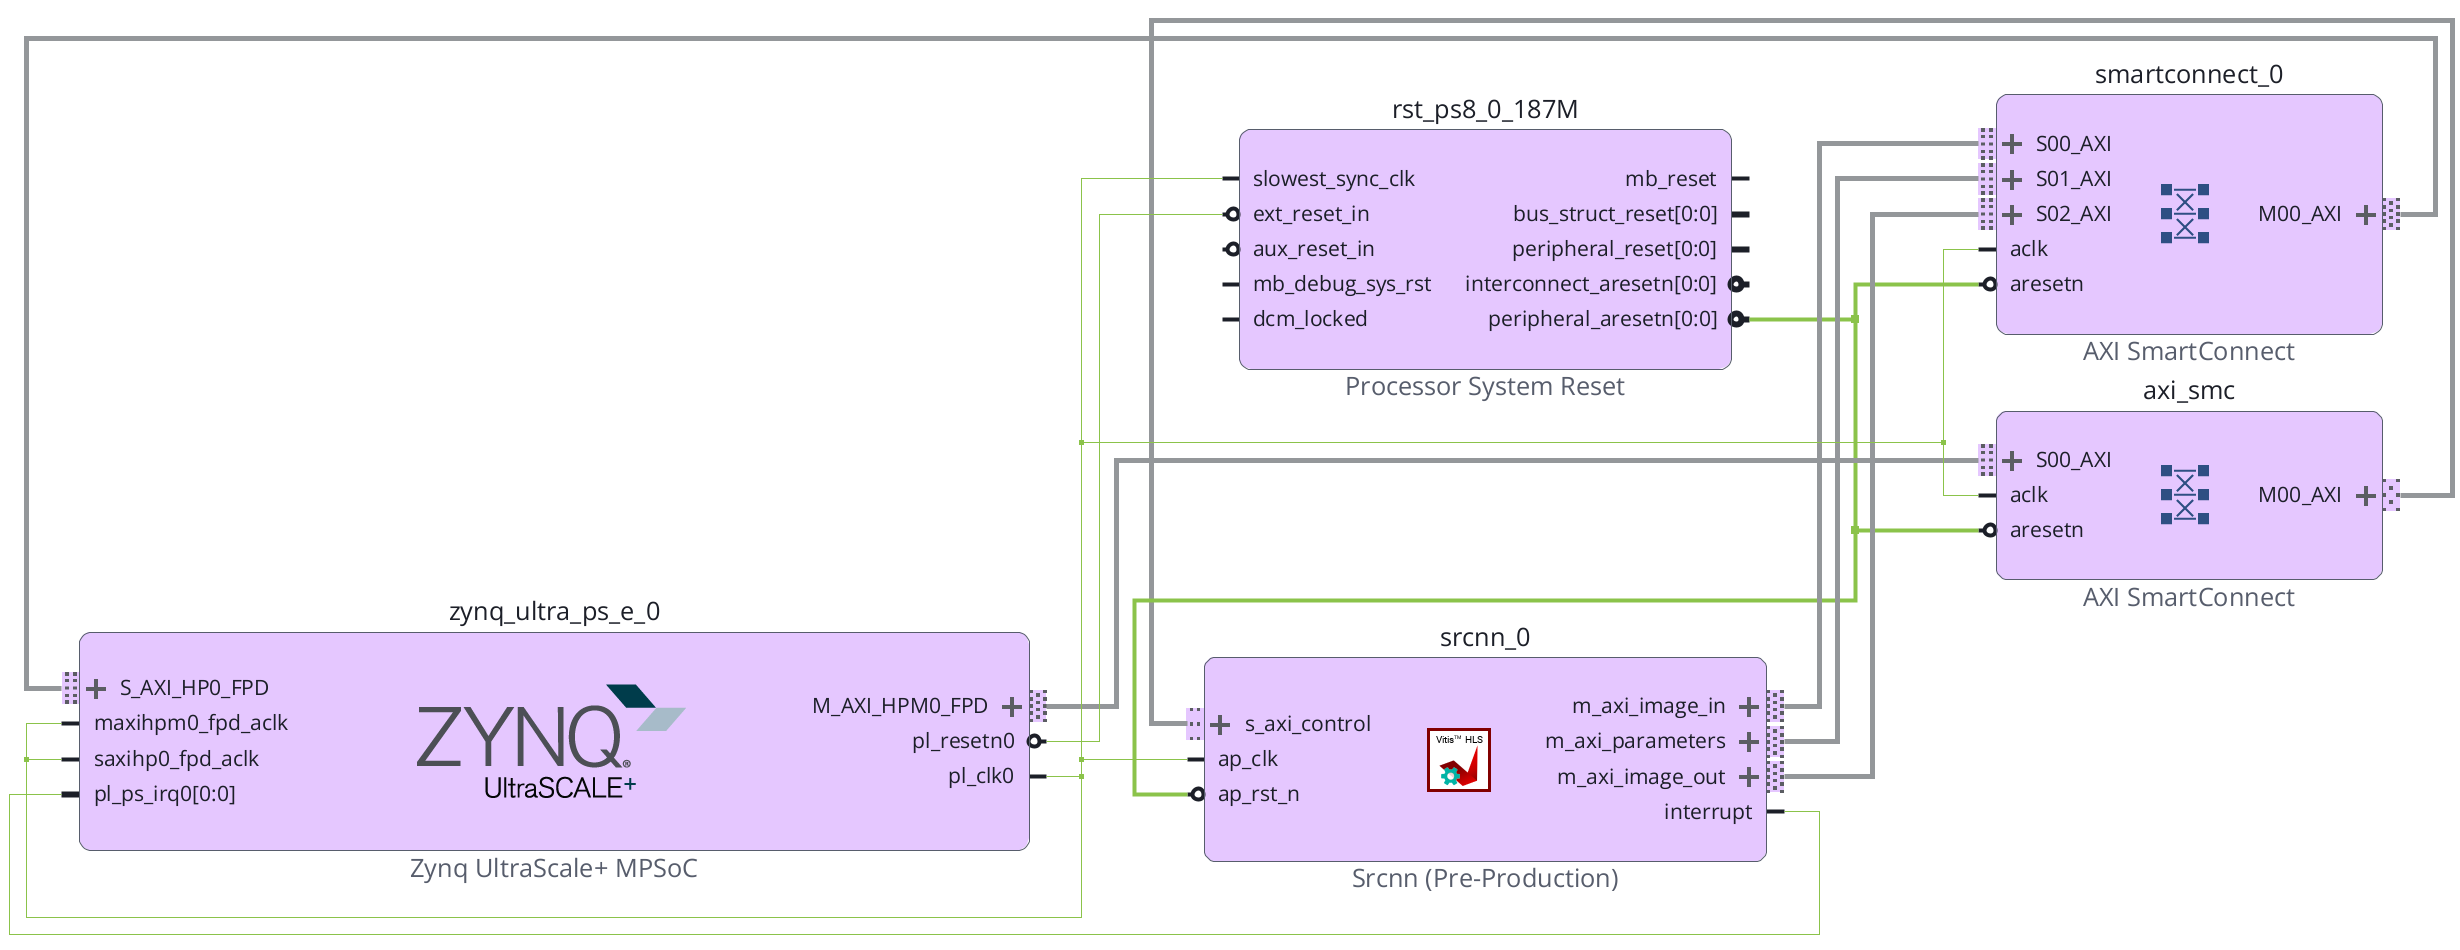
\includegraphics[width=\figw]{figures/fig07-block-design-hp0.png}
\caption{Vivado block design of the first PS+PL deployment. The PS reaches the SRCNN control registers through M\_AXI\_HPM0\_FPD and a control SmartConnect; the three SRCNN AXI masters (image\_in, parameters, image\_out) share S\_AXI\_HP0\_FPD through a second SmartConnect.}
\label{fig:7}
\end{figure}

The post-route resource utilization of this design is given in Table~\ref{tab:11}.

\begin{table}[!htbp]
\centering
\footnotesize
\caption{Post-route resource utilization of the C22 design on the xck26-sfvc784-2LV-c device, as reported by Vivado after implementation.}
\label{tab:11}
\begin{tabular}{lrrr}
\toprule
Resource & Usage & Available & Utilization (\%) \\
\midrule
LUT & 63,078 & 117,120 & 53.86\% \\
FF & 106,341 & 234,240 & 45.40\% \\
DSP & 1,032 & 1,248 & 82.69\% \\
BRAM36 & 54.5 & 144 & 37.85\% \\
Used CLB & 14,309 & 14,640 & 97.74\% \\
\bottomrule
\end{tabular}
\end{table}

Vivado implements the integrated system at the PL0 period it derives from the PS preset, 5.333 ns (187.5 MHz). At this constraint the post-route report shows WNS +0.043 ns, WHS +0.010 ns, TNS = THS = 0, no unconstrained endpoints, all 181,382 nets routed and zero routing errors, so the final gate of Section~\ref{sec:3} is satisfied by the integrated system as well as by the stand-alone IP (C22: WNS +0.013 ns at 5 ns). The worst setup path lies in the Conv1 Winograd engine (4.893 ns data path, of which 3.127 ns logic and 1.766 ns routing), and the slack of 43 ps shows the timing margin leaved by the T = 4 is quite small. Vivado's power model estimates 5.8 W on chip (5.5 W dynamic, of which 2.6 W is the PS). The resource utilization in Table~\ref{tab:11} shows why no further growth of the design is possible: the DSPs are 82.7 \% used and the CLBs 97.7 \%, so the device is effectively full.

\subsection{Functional verification on the board}\label{sec:5.2}

The bitstream and the hardware handoff file were loaded on the KV260 through PYNQ 3.0.1. One invocation proceeds as follows: contiguous buffers are allocated for the input image, the six parameter arrays and the output; the float32 weights and biases are copied in the exact layout of the HLS function signature; the output buffer is filled with NaN; all buffers are flushed to DDR; the buffer addresses are written to the IP's control registers; the IP is started and \texttt{AP\_DONE} is polled; the output buffer is invalidated and read back; and the result is compared against the reference. Two timers wrap this sequence: \emph{start-to-done} covers only the interval between the start write and the observation of \texttt{AP\_DONE}, and \emph{with cache and copy} covers the whole invocation including cache maintenance, the copy of the output and the NaN/Inf check.

We compared the output content of the FPGA board in two ways: first, a bit-by-bit comparison with the results computed by co-simulation to verify whether the hardware computation results are correct. Image quality is then measured against the float golden output and the ground-truth image as MSE and PSNR; this tells us what the fixed-point design costs in quality. Table~\ref{tab:12} traces each specification and gate from Section~\ref{sec:3} to the on-board evidence that closes it.

\begin{table}[!htbp]
\centering
\footnotesize
\caption{Specifications and acceptance gates from Section~\ref{sec:3}}
\label{tab:12}
\begin{tabularx}{\linewidth}{L{4.6cm}L{3.1cm}Y}
\toprule
Specification / gate (Section~\ref{sec:3}) & Expected & Measured on the board \\
\midrule
\texttt{srcnn} signature with float arrays, runtime-loaded parameters & Parameters read from DDR on every call & Constant-image test with altered weights and biases returns the analytically expected value 104/256; restoring the original parameters restores the bit-exact output \\
Bit-exact against the fixed-point reference on all 13 Set14 images & 13 / 13 & 13 / 13, plus Butterfly (Set5) \\
Mean PSNR on Set14 no worse than $-$0.1 dB against float & $\ge$ $-$0.1 dB & 29.083 dB on the board, identical to the C17 co-simulation record (29.083 dB); $-$0.076 dB against the float golden (Section~\ref{sec:4}) \\
Post-route timing met, zero unrouted nets & Met at the implemented clock & Met at 5.333 ns: WNS +0.043 ns, WHS +0.010 ns, 0 route errors; +0.074 ns with the cycle monitor added \\
Primary metric: milliseconds per frame & 1.365 ms at 200 MHz (RTL $\times$ routed clock) & 2.938 ms hardware time at 166.665 MHz \\
\bottomrule
\end{tabularx}
\end{table}

Table~\ref{tab:13} lists the per-image result of the Set14 run. The mean PSNR against the ground truth matches the co-simulation record to three decimals. The per-image start-to-done time is essentially constant at 2.95 ms, as expected.

\begin{table}[!htbp]
\centering
\footnotesize
\caption{Set14 verification on the KV260 (output on HP1, 166.665 MHz). Bit-exact is against the fixed-point reference output of each image; PSNR is against the ground-truth image, for the bicubic input and for the SRCNN output; gain is the difference. Time is the Python start-to-done interval of the single run.}
\label{tab:13}
\begin{tabular}{llrrrr}
\toprule
Image & Bit-exact & PSNR input (dB) & PSNR output (dB) & Gain (dB) & Start-to-done (ms) \\
\midrule
baboon & True & 27.36 & 27.89 & +0.53 & 2.953 \\
barbara & True & 24.90 & 24.97 & +0.07 & 2.951 \\
bridge & True & 25.23 & 26.18 & +0.95 & 2.954 \\
coastguard & True & 26.30 & 26.82 & +0.52 & 2.950 \\
face & True & 32.68 & 33.34 & +0.66 & 2.952 \\
flowers & True & 25.70 & 27.30 & +1.60 & 2.952 \\
foreman & True & 33.20 & 35.48 & +2.28 & 2.950 \\
lenna & True & 29.17 & 30.78 & +1.61 & 2.950 \\
man & True & 26.06 & 27.09 & +1.03 & 2.952 \\
monarch & True & 24.58 & 27.97 & +3.39 & 2.952 \\
pepper & True & 32.05 & 33.35 & +1.31 & 2.950 \\
ppt3 & True & 26.68 & 29.34 & +2.66 & 2.951 \\
zebra & True & 24.74 & 27.56 & +2.82 & 2.952 \\
\textbf{Mean} & \textbf{13 / 13} & \textbf{27.59} & \textbf{29.08} & \textbf{+1.49} & \textbf{2.951} \\
\bottomrule
\end{tabular}
\end{table}

The \textbf{parameter reload test} zeroes all weights, sets the biases to 0.5, 0.25 and 0.125, places a single 0.25, 0.5 and 0.5 at the centre of one kernel in each layer, and feeds a constant 0.5 image; the expected output is then a constant (0.5 $\times$ 0.25 + 0.5) $\times$ 0.5 + 0.25 = 0.5625 $\rightarrow$ $\times$ 0.5 + 0.125 = 104/256 after quantization, and the board returns exactly this value, which shows that the parameters are read from DDR on every call rather than cached from the first. Restoring the original parameters restores the bit-exact Butterfly output. The \textbf{NaN pre-fill} of the output buffer ensures that an IP that never writes a pixel is detected, since the check fails on any remaining NaN.

\subsection{Performance debugging}\label{sec:5.3}

Functionally the design was therefore correct from the first bitstream, but the inference time of the initial deployment was 5.05 ms per image, 3.7$\times$ the 1.365 ms of the RTL reference. Three causes were suspected: the operating clock, the Python control and polling overhead, and the AXI/DDR access path. The following subsections take them in order.

\subsubsection{Clock frequency}\label{sec:5.3.1}

First, we read the clock frequency: on the board, PYNQ was used to read \texttt{Clocks.fclk0\_mhz}, which returned \texttt{124.99875 MHz}. This is reasonable. Although PL0's requested frequency was set to \texttt{200 MHz} in Vivado, the actual configured frequency recorded in the HWH is \texttt{187.498123 MHz}, with the clock source being the IOPLL and a divider ratio of \texttt{8$\times$1}. \texttt{IOPLL\_CTRL = 0x13c00} corresponds to a multiplier of 60 with the output divided by 2. Therefore, based on a reference clock of approximately \texttt{33.333 MHz}, the on-board IOPLL runs at about \texttt{1000 MHz}, and the PL0 frequency is about \texttt{1000 $\div$ 8 = 125 MHz}. In contrast, the Vivado preset uses an IOPLL of about 1500 MHz, so the same divider yields about \texttt{187.5 MHz}. At the 125 MHz actually configured, the 273,023 RTL cycles would take 2.18 ms, so the clock alone explains less than half of the 5.05 ms.

We changed the divider to 6 and observed that the time was further reduced to 3.98 ms; Table~\ref{tab:14} compares the two clock configurations.

\begin{table}[!htbp]
\centering
\footnotesize
\caption{PL0 clock configuration before and after changing the IOPLL output divider from 8 to 6. The frequency is derived from the PLL control registers read on the board; the time is the median Python start-to-completion time over repeated runs.}
\label{tab:14}
\begin{tabular}{lll}
\toprule
Parameter & Before Modification & After Modification \\
\midrule
PL0 divider & 8$\times$1 & 6$\times$1 \\
Register-derived frequency & 124.99875 MHz & 166.665 MHz \\
Median time from start to completion & 5.005195 ms & 3.984220 ms \\
Output consistent with reference & True & True \\
\bottomrule
\end{tabular}
\end{table}

We deliberately stopped at a divider of 6 rather than going to 5 (200 MHz). The purpose of this step was to measure how strongly the on-board time depends on the PL clock, not to reach the design clock; the PL0 clock also drives the AXI interconnect, so a change cannot be attributed to the compute logic alone, and a run at 200 MHz would first need its own timing verification on the integrated system. To separate clock-bound from clock-independent time, we swept the divider over 10, 8 and 6 in alternating order (four sweeps, five timed runs each after a warm-up) with the three AXI masters still sharing HP0; Table~\ref{tab:15} gives the result.

\begin{table}[!htbp]
\centering
\footnotesize
\caption{PL0 clock sweep with the three AXI masters sharing HP0. Median, minimum and maximum of 20 start-to-done measurements per frequency; software-equivalent cycles = median time $\times$ frequency; RTL reference = 273,023 cycles $\div$ frequency.}
\label{tab:15}
\begin{tabular}{lrrrR{2.3cm}R{1.9cm}}
\toprule
PL0 clock (MHz) & Median (ms) & Min (ms) & Max (ms) & Software-equivalent cycles & RTL reference (ms) \\
\midrule
99.999 & 5.955 & 5.950 & 5.957 & 595,460 & 2.730 \\
124.999 & 4.994 & 4.992 & 4.997 & 624,290 & 2.184 \\
166.665 & 3.982 & 3.977 & 3.984 & 663,688 & 1.638 \\
\bottomrule
\end{tabular}
\end{table}

From the output, we found: The time falls with frequency, but not in proportion: the software-equivalent cycle count rises from 595 k to 664 k as the clock rises, so a part of the time does not scale with the PL clock. A linear fit \emph{t = a + b / f} to the three points gives \emph{b} $\approx$ 493 k cycles and \emph{a} $\approx$ 1.0 ms: roughly 493 k cycles of the work run on the PL clock, and about 1 ms per frame is spent in a path whose latency is fixed in absolute time, which points at the PS-side interconnect and the DDR controller rather than at the accelerator. This indicates that AXI/DDR overhead is what dominates the hardware execution time, the hardware counters below confirm it.

\subsubsection{Software overhead: register access and polling}\label{sec:5.3.2}

We then looked at the time spent on Python reads/writes and polling. A single read via \texttt{ip.read(0x00)} took 7.807 \textmu{}s, compared with 2.353 \textmu{}s via \texttt{ip.mmio.array[0]}; both are negligible against a frame time of several milliseconds. To test whether the polling itself disturbs the execution (for example through MMIO traffic on the same interconnect), we delayed the first status read by 0, 1, 2 and 3 ms after the start write, ten repeats each, and recorded the completion time and the number of status reads (Table~\ref{tab:16}).

\begin{table}[!htbp]
\centering
\footnotesize
\caption{Effect of delaying the first status read after the start write (HP0 configuration, 166.665 MHz; medians of 10 runs). The completion time is unchanged while the number of polling reads falls from 606 to 135, so polling does not affect the execution.}
\label{tab:16}
\begin{tabular}{lrrr}
\toprule
Requested first wait (ms) & Actual first read (ms) & Median completion (ms) & Median polling reads \\
\midrule
0 & 0.013 & 3.981 & 606.5 \\
1 & 1.106 & 3.984 & 443.0 \\
2 & 2.100 & 3.984 & 288.5 \\
3 & 3.100 & 3.983 & 135.0 \\
\bottomrule
\end{tabular}
\end{table}

The completion time is identical to within 3 \textmu{}s regardless of the polling density, so neither register access nor polling contributes to the gap. Software overhead is therefore confined to the part of the invocation outside the start-to-done interval, which is reported separately in Table~\ref{tab:20}.

\subsubsection{Hardware cycle count}\label{sec:5.3.3}

Neither the clock frequency nor the software path can account for the gap between on-board and simulated execution times, and the clock sweep suggested a clock-independent component. It passively observes the write channel of the SRCNN \texttt{s\_axi\_control} slave (AWADDR, AWVALID/AWREADY, WDATA, WSTRB, WVALID/WREADY) and the SRCNN \texttt{interrupt} output. The counter starts on the clock edge at which a write to \texttt{AP\_CTRL} with bit 0 set is accepted, counts PL0 cycles, and stops and latches on the edge at which the completion interrupt is observed. The 32-bit count and a status word (completion sequence number, busy, overflow and error flags) are brought out through a dual-channel AXI GPIO on the control SmartConnect, which the PS reads after each run; the sequence number lets the software confirm that the count belongs to the frame just launched. The interval includes a few cycles of control and interrupt latency on either side of the true \texttt{ap\_start} $\rightarrow$ \texttt{ap\_done} window, which is negligible against the hundreds of thousands of cycles in question. The new build was re-checked: WNS +0.074 ns, THS = TPWS = 0. The block design with the cycle monitor is shown in Figure~\ref{fig:8}.

\begin{figure}[!htbp]
\centering
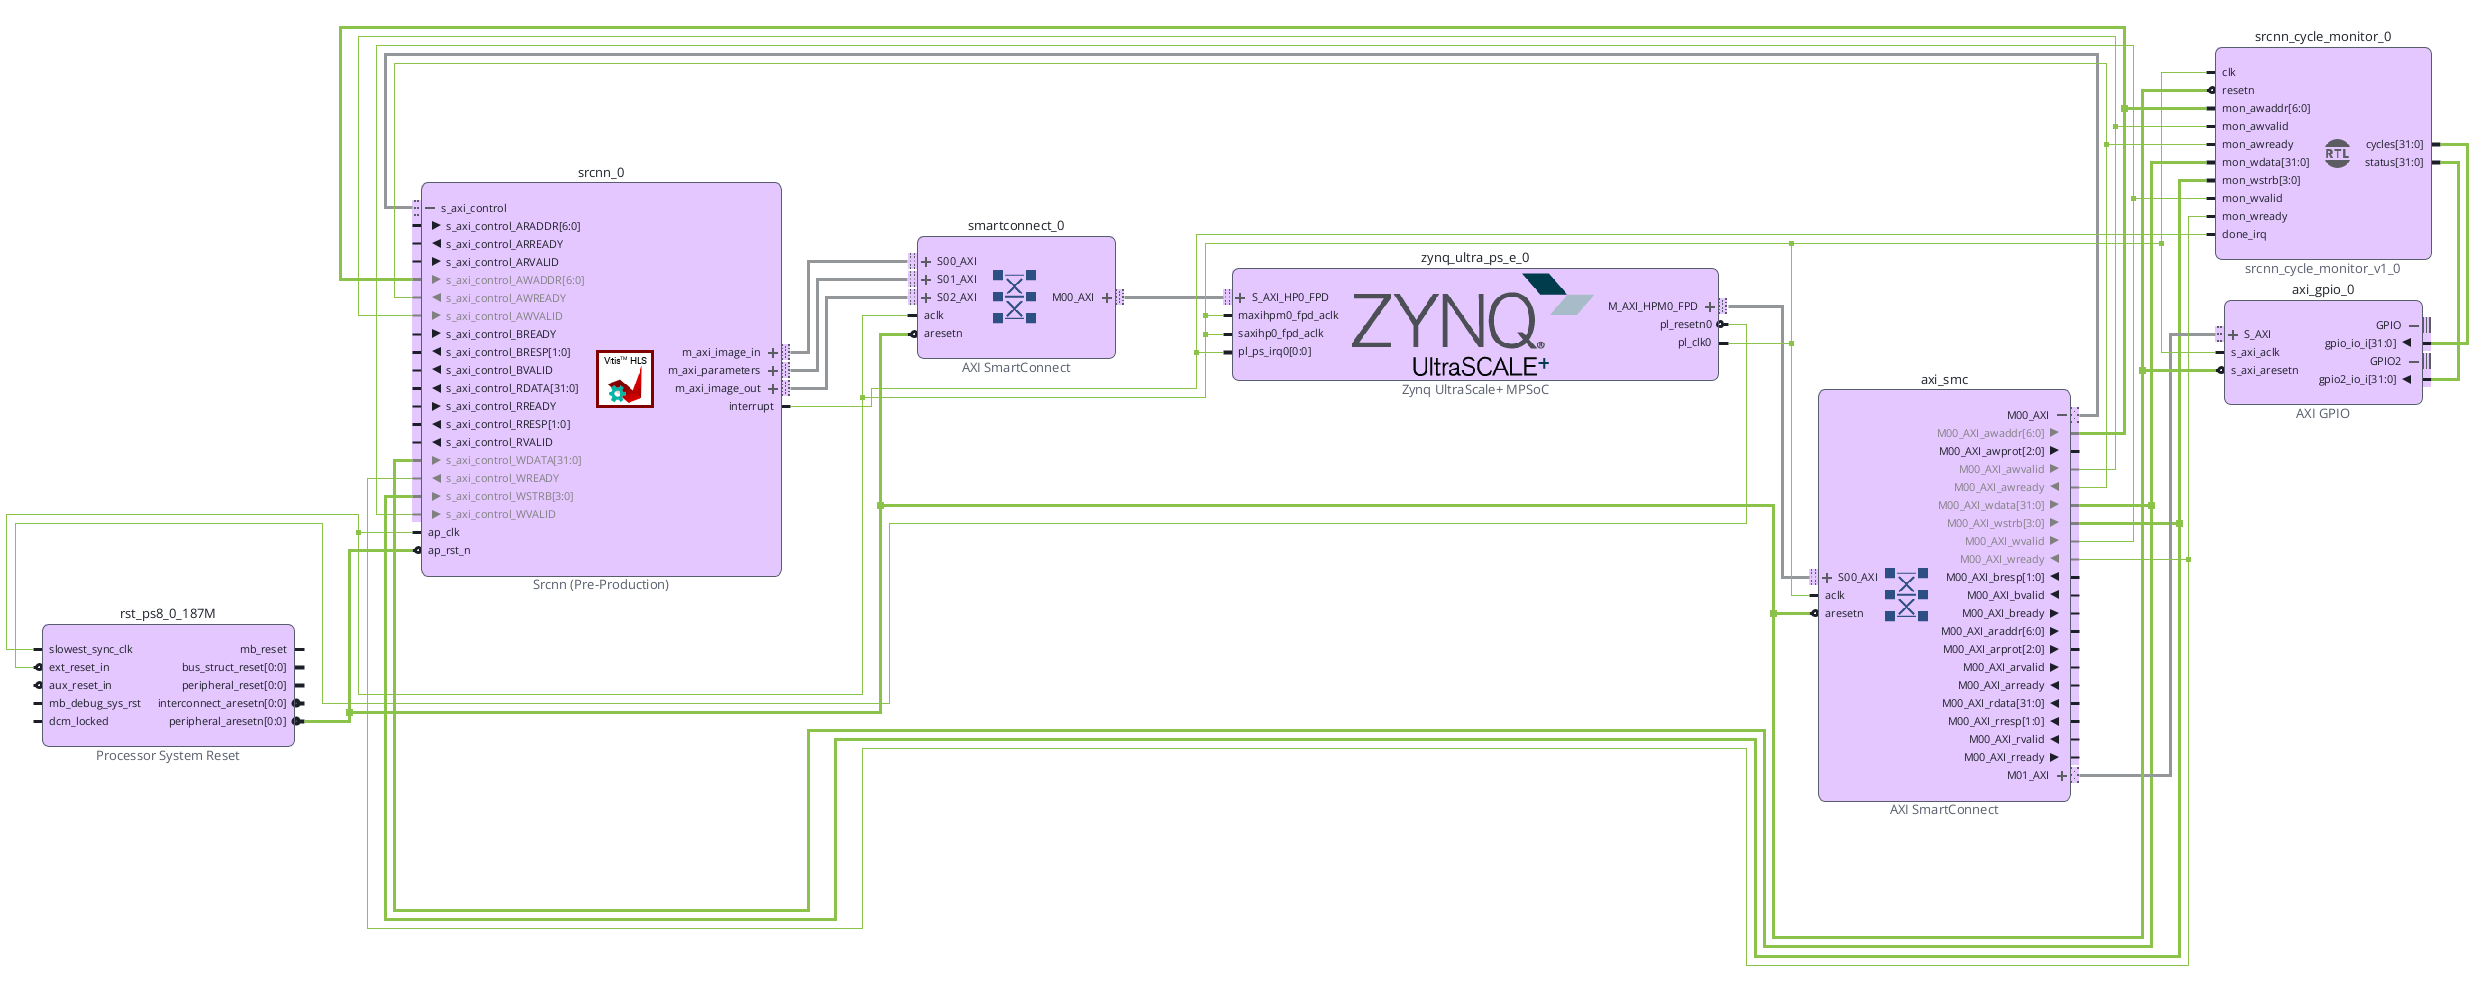
\includegraphics[width=\figw]{figures/fig08-block-design-cycle-monitor.png}
\caption{Block design with the hardware cycle-monitor module. The counter starts on the start write to the SRCNN s\_axi\_control interface and stops and latches on the SRCNN completion interrupt, so the count excludes all PYNQ software overhead.}
\label{fig:8}
\end{figure}

The measurement it produced is summarized in Table~\ref{tab:17}.

\begin{table}[!htbp]
\centering
\footnotesize
\caption{Hardware-timed execution of one frame measured by the cycle monitor at 166.665 MHz, compared with the Python-timed start-to-completion interval.}
\label{tab:17}
\begin{tabular}{ll}
\toprule
Metric & Result \\
\midrule
Operating frequency & 166.665 MHz \\
Hardware count & 668,366 cycles \\
Hardware-timed interval & 4.010236 ms \\
Python start-to-completion time & 4.033060 ms \\
Difference between the two & 22.824 \textmu{}s \\
Output bit-exact with reference & True \\
\bottomrule
\end{tabular}
\end{table}

The original RTL reference is 273,023 cycles, while 668,366 cycles were measured on the board --- an excess of 395,343 cycles. RTL co-simulation results show that the Dataflow pipeline of the three SRCNN convolution layers already achieves high computational unit utilization, and the RTL execution cycles are close to the HLS estimate. Therefore, the time gap relative to simulation is caused at the hardware execution level. Considering that on-board operation also involves the AXI interconnect, HP ports, and DDR controller, we further examine the external memory access path to determine whether there is additional data transfer waiting.

\subsubsection{Memory access path}\label{sec:5.3.4}

To check whether the shared AXI access path introduces additional wait time, we tried splitting the output path: the image output was connected to the 128-bit \texttt{S\_AXI\_HP1\_FPD} through an independent SmartConnect, while the input and parameters still access HP0 through the original SmartConnect. The modified block design is shown in Figure~\ref{fig:9}.

\begin{figure}[!htbp]
\centering
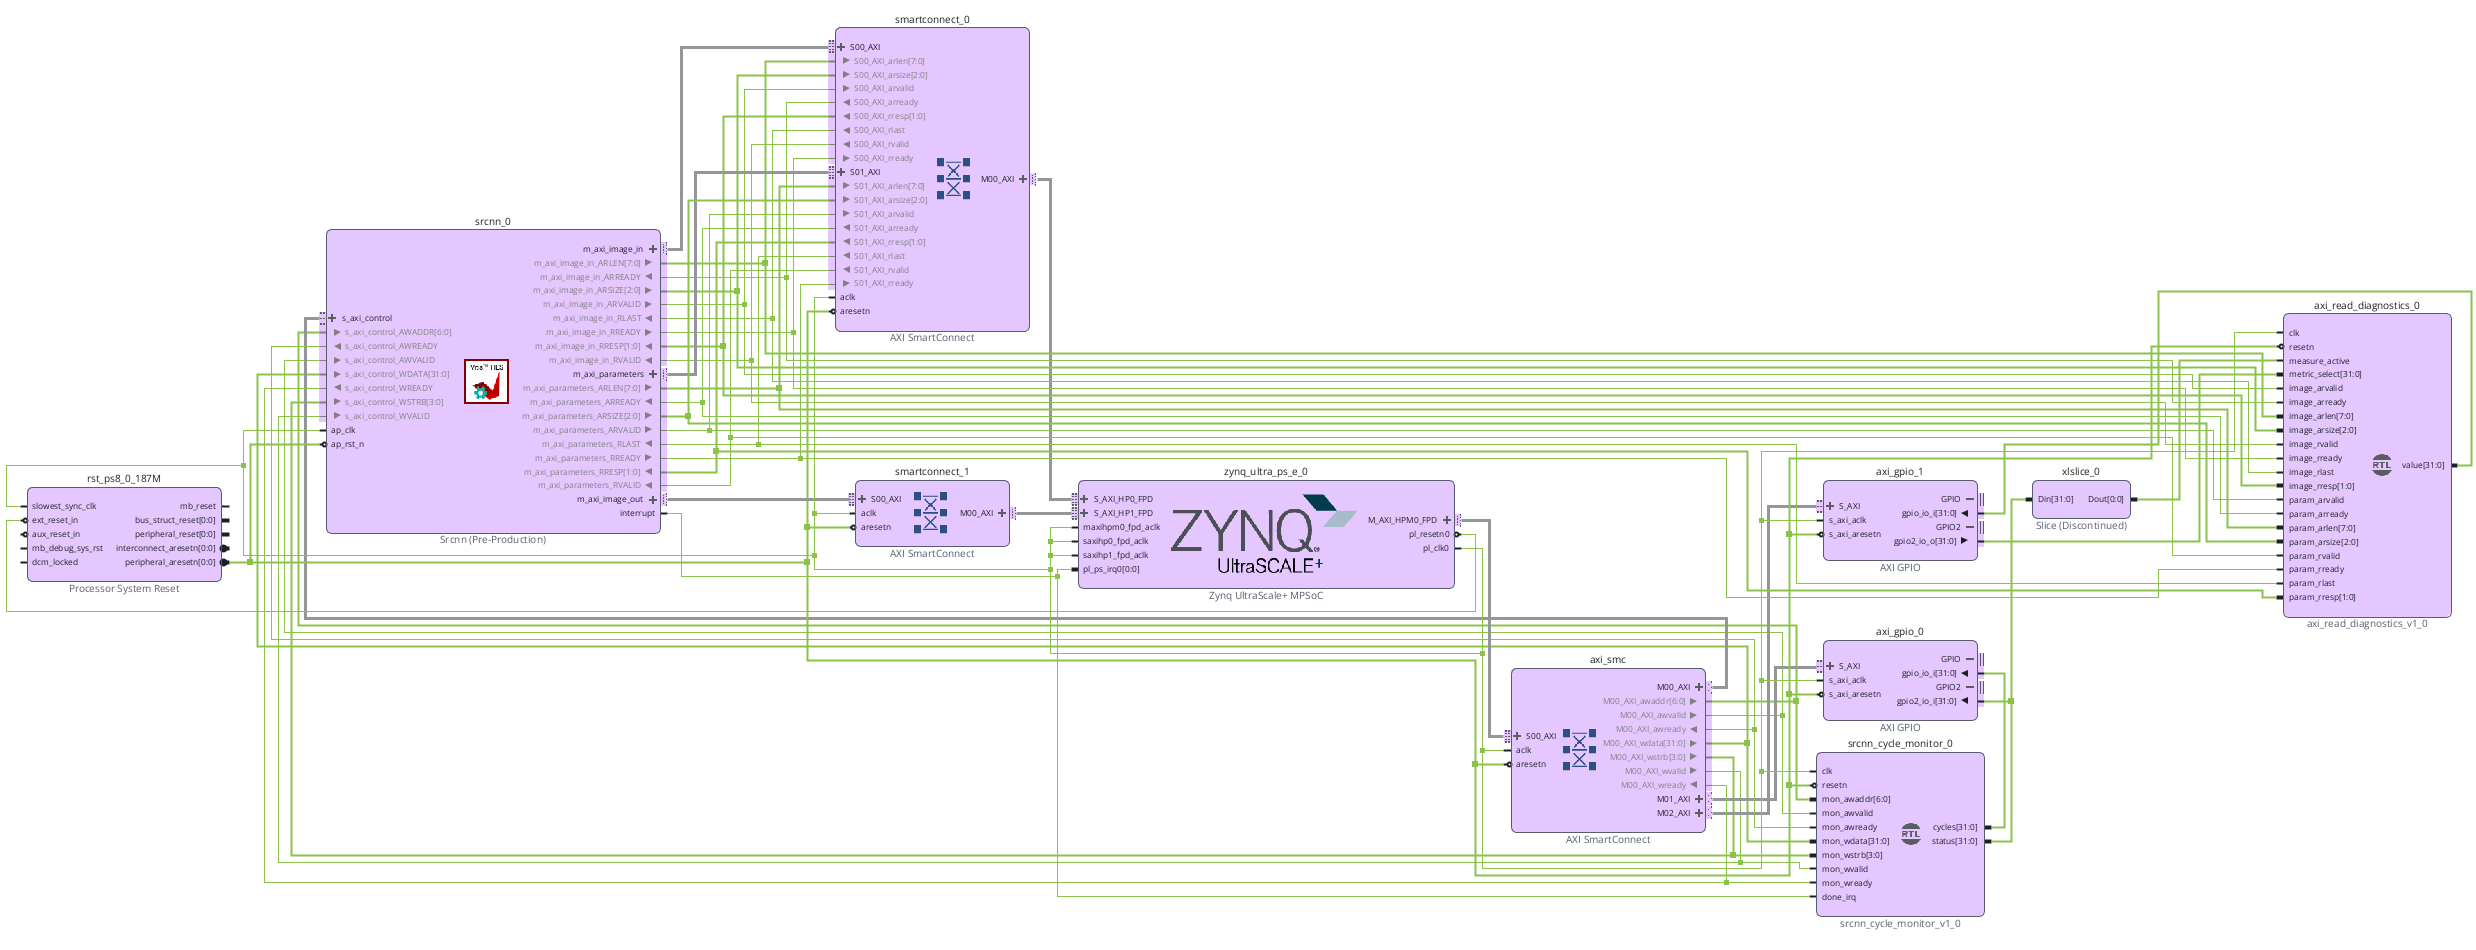
\includegraphics[width=\figw]{figures/fig09-block-design-hp1.png}
\caption{Block design with the output path separated: m\_axi\_image\_out reaches DDR through its own SmartConnect and S\_AXI\_HP1\_FPD, while m\_axi\_image\_in and m\_axi\_parameters keep sharing S\_AXI\_HP0\_FPD. The cycle monitor from Figure~\ref{fig:8} is retained.}
\label{fig:9}
\end{figure}

The design still passed verification at 166.665 MHz, and the on-board execution time dropped to 2.94 ms, with the cycle count reduced to 489,585. Table~\ref{tab:18} compares the two configurations over repeated runs; separating the output path reduces the hardware cycle count by 26.6 \%.

\begin{table}[!htbp]
\centering
\footnotesize
\caption{On-board cycle count and hardware time per frame with the three AXI masters sharing HP0 (Figure~\ref{fig:8}) versus the output on a dedicated HP1 port (Figure~\ref{fig:9}). Minimum, median and maximum are taken over repeated runs at 166.665 MHz.}
\label{tab:18}
\begin{tabular}{lll}
\toprule
Metric & Three interfaces sharing HP0 & Output on dedicated HP1 \\
\midrule
Minimum cycles & 666,988 & 489,423 \\
Median cycles & 667,084 & 489,584.5 \\
Maximum cycles & 668,015 & 497,301 \\
hardware time & 4.003 ms & 2.938 ms \\
Output bit-exact & True & True \\
\bottomrule
\end{tabular}
\end{table}

This is one of the main reasons why the actual execution time exceeds the simulated time. AMD's official documentation also notes that the Zynq UltraScale+'s HP interfaces reach the DDR controller through an interconnect network, and that accesses are subject to arbitration and QoS mechanisms.\footnote{AMD Xilinx wiki, \emph{Traffic Shaping of HP Ports on Zynq UltraScale+}: \url{https://xilinx-wiki.atlassian.net/wiki/spaces/A/pages/688128001/Traffic\%2BShaping\%2Bof\%2BHP\%2BPorts\%2Bon\%2BZynq\%2BUltraScale}}

To further pinpoint the problem, we added an AXI read-path statistics module. For each of the image and parameter ports it observes ARVALID/ARREADY, ARLEN, ARSIZE, RVALID/RREADY, RLAST and RRESP, and accumulates sixteen counters over the busy window of the cycle monitor: window cycles, accepted read requests, returned data beats, completed bursts, requested beats and bytes, cycles of AR back-pressure (ARVALID without ARREADY), cycles of R back-pressure (RVALID without RREADY, the HLS consumer not accepting data), cycles with a request outstanding but no RVALID, the maximum number of outstanding transactions, first-AR and last-RLAST cycle, non-OKAY responses, orphan RLASTs and outstanding transactions at the end of the window. The counters are selected and read through a second AXI GPIO after the frame completes; the read-back script checks the frame sequence number, that requested beats equal returned beats, and that no response errors or outstanding transactions remain before the numbers are used. The average burst length is returned beats divided by completed bursts. The block design with this module added is shown in Figure~\ref{fig:10}.

\begin{figure}[!htbp]
\centering
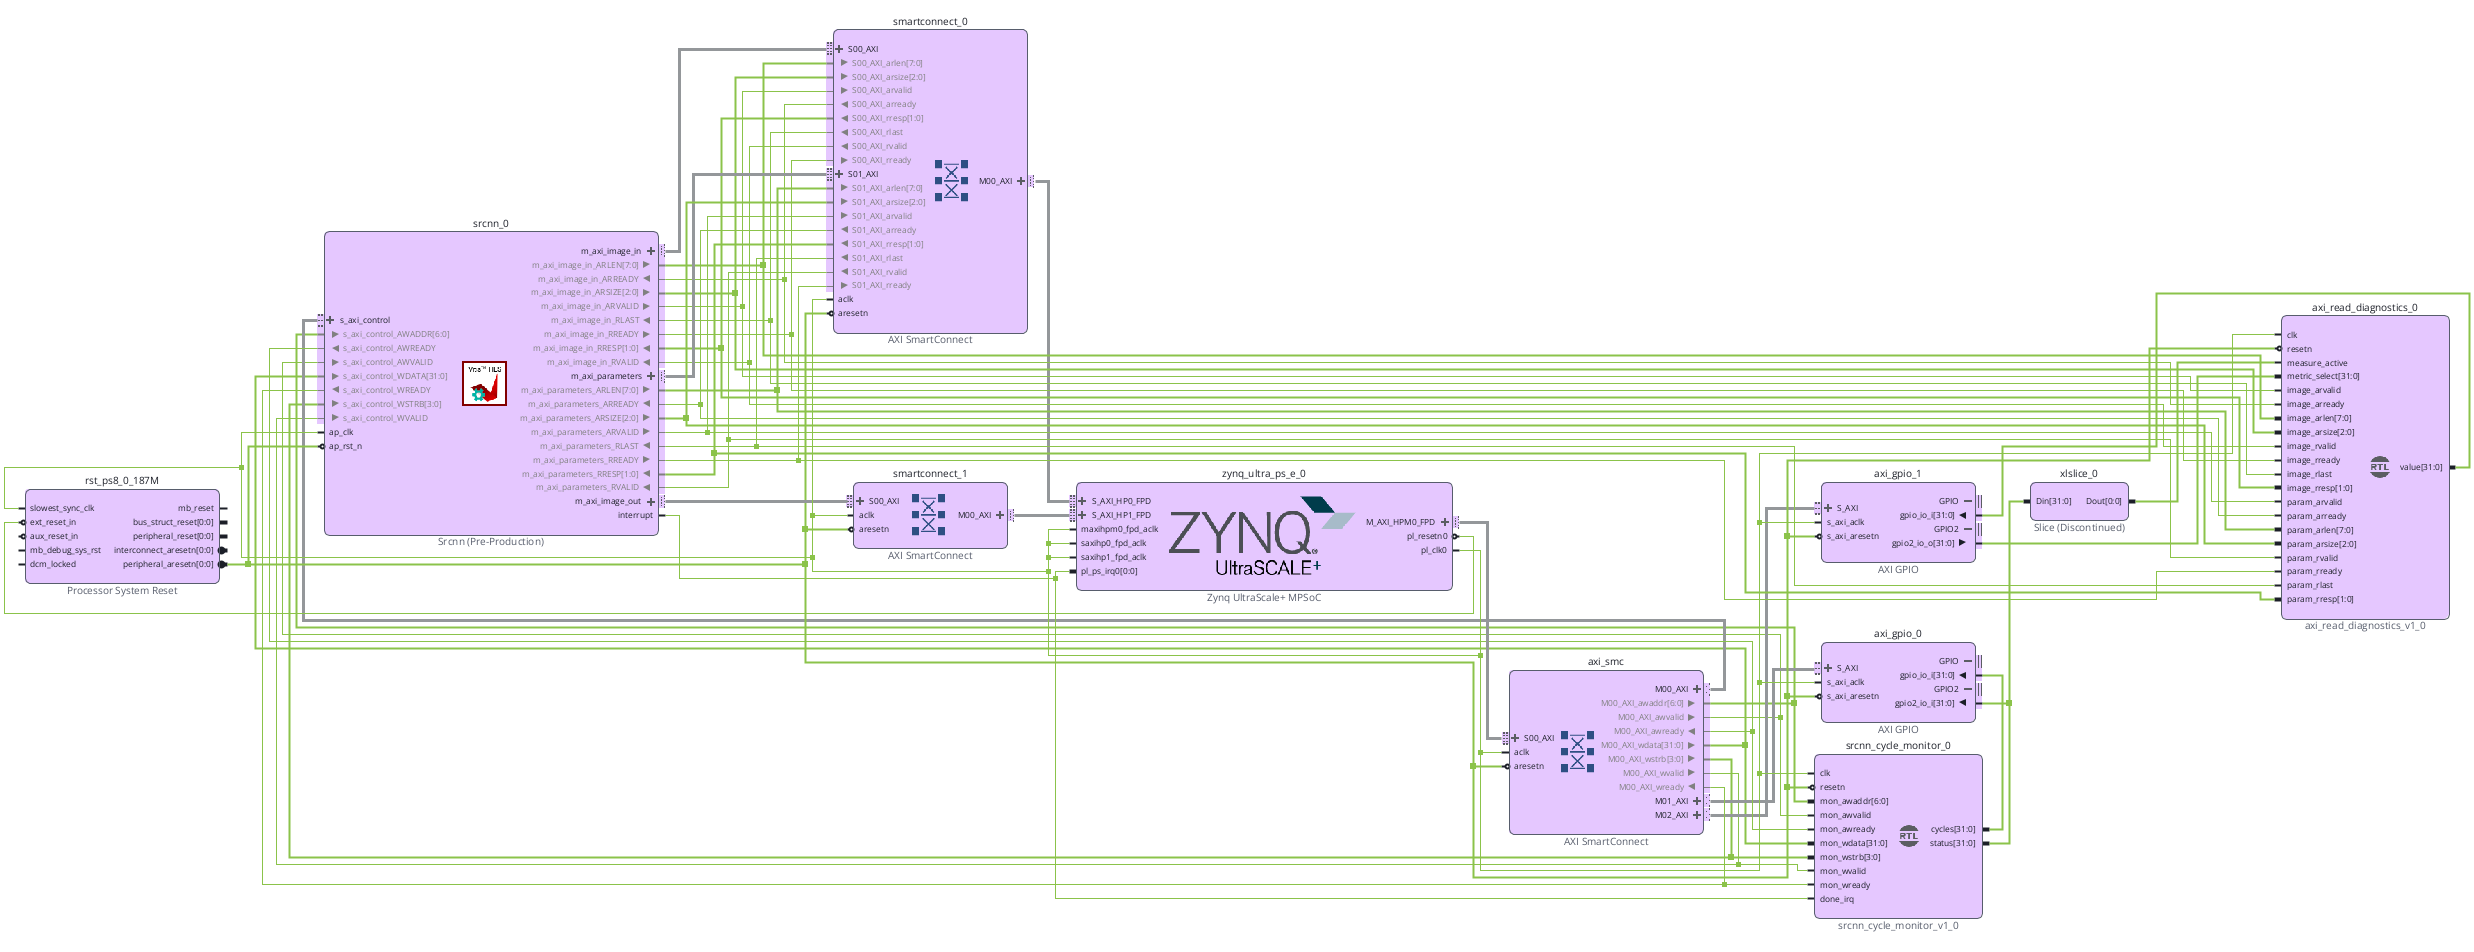
\includegraphics[width=\figw]{figures/fig10-block-design-axi-stats.png}
\caption{Block design with the AXI read-path statistics module attached to the image and parameter read channels on HP0. The module counts total cycles, cycles with an outstanding read request but no valid data, and the average burst length of each channel; the output path remains on HP1 as in Figure~\ref{fig:9}.}
\label{fig:10}
\end{figure}

With this module in place, the run on the FPGA board executed a total of 494,066 cycles, taking about 2.964 ms. Among these, the image input channel had outstanding read requests without valid data returned during approximately 77.7\% of the statistics window cycles, indicating that there are substantial read-response gaps during image reading. In addition, the average burst length of both read channels was 1 beat, showing that the actual AXI reads did not form multi-beat bursts. Although we set \texttt{max\_read\_burst\_length=256} in HLS, this parameter only specifies the maximum allowed burst length; the actual bursts are not controlled by this parameter.

The section of the AMD official documentation mentioned earlier, which discusses the impact of AXI access patterns on the transfer performance of the Zynq UltraScale+ HP interfaces, also supports our hypothesis: the currently observed read-response gaps may be related to the transfer overhead caused by single-beat transactions, as well as the access latency in the AXI interconnect, the HP interfaces, and the DDR controller.

\subsection{Final on-board result}\label{sec:5.4}

\begin{table}[!htbp]
\centering
\footnotesize
\caption{Per-frame latency of the SRCNN accelerator at each stage of development and deployment. The RTL reference is co-simulated cycles $\times$ 5 ns; all other rows are measured on the KV260.}
\label{tab:19}
\begin{tabularx}{\linewidth}{llY}
\toprule
Stage & Latency & Description \\
\midrule
Original floating-point Baseline & 2.238 s & Measured on board \\
Final architecture RTL reference & 1.365 ms & Simulation cycles $\times$ 5 ns \\
First on-board deployment & 5.05 ms & Initial clock configuration \\
After clock adjustment & 3.984 ms & 166.665 MHz \\
After input/output splitting & 2.938 ms & Final on-board hardware time \\
\bottomrule
\end{tabularx}
\end{table}

Table~\ref{tab:19} summarizes the execution latency of the SRCNN accelerator across different development and deployment stages. The original floating-point baseline requires 2.238 s to run one frame on the board. After optimizations such as fixed-point quantization, Winograd convolution, and the Dataflow pipeline, the final architecture achieves an estimated execution time of 1.365 ms in RTL simulation. However, the actual latency of the first on-board deployment is 5.05 ms, significantly higher than the simulation result.

By adjusting the PL clock frequency and separating the output data path from the shared HP0 interface to an independent HP1 interface, the on-board execution latency is reduced to 2.938 ms, a 762$\times$ speedup over the original baseline measured on the same board. Table~\ref{tab:20} characterises this final configuration over 20 consecutive runs, and Figure~\ref{fig:11} shows its reconstructed image.

\begin{table}[!htbp]
\centering
\footnotesize
\caption{Timing of the final configuration (output on HP1, PL0 at 166.665 MHz) over 20 consecutive Butterfly runs, all bit-exact. Start-to-done is the Python-timed interval from the start write to the observation of AP\_DONE; with cache and copy is the complete invocation. The hardware-timed value from the cycle monitor (Table~\ref{tab:18}) is 2.938 ms.}
\label{tab:20}
\begin{tabular}{llrl}
\toprule
Quantity & Min & Median & Max \\
\midrule
Start-to-done (ms) & 2.949 & 2.951 & 2.958 \\
With cache and copy (ms) & 5.907 & 5.976 & 6.549 \\
Hardware cycles (cycle monitor) & 489,423 & 489,584.5 & 497,301 \\
RTL reference at 166.665 MHz (ms) & --- & 1.638 & --- \\
\bottomrule
\end{tabular}
\end{table}

The Python start-to-done median of 2.951 ms exceeds the hardware-timed 2.938 ms by 13 \textmu{}s, which is the cost of the start write and the last status read; the two timers agree, so the software timer can be used as a proxy for hardware time in the earlier experiments where the cycle monitor was not yet present.

\begin{figure}[!htbp]
\centering
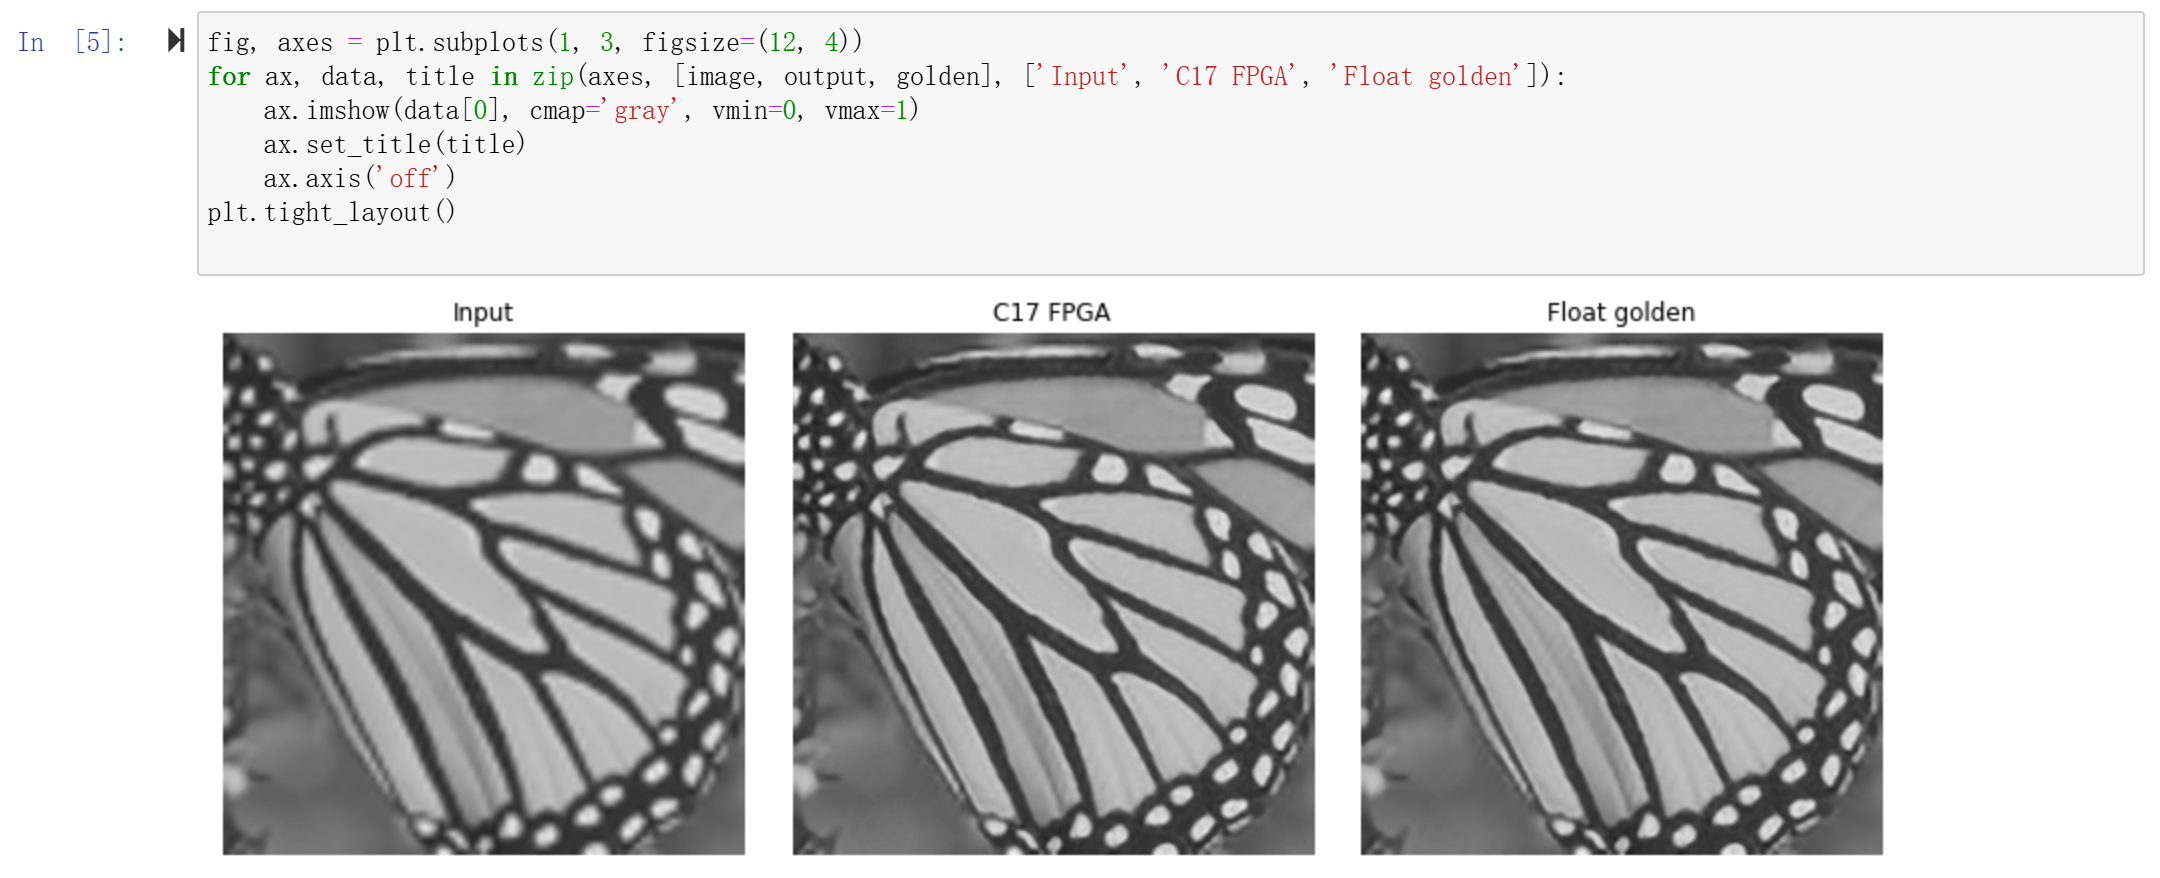
\includegraphics[width=\figw]{figures/fig11-butterfly.png}
\caption{Butterfly: bicubic input (left), output of the final version running on the KV260 (centre, output on HP1, 166.665 MHz) and float golden (right). The board output is bit-exact with the fixed-point reference; MSE against the float golden is 1.77 $\times$ 10\textsuperscript{-5}.}
\label{fig:11}
\end{figure}

Figure~\ref{fig:11} shows the Butterfly input, the board output and the float golden side by side; the board output is bit-exact with the fixed-point reference and its MSE against the float golden is \texttt{1.77065 $\times$ 10\textsuperscript{-5}}. The median hardware execution time is \texttt{2.938 ms} (489,584.5 cycles, about 340 frames per second). A complete invocation takes about 6 ms (median 5.98 ms, Table~\ref{tab:20}); the 3 ms beyond the hardware time is spent in the software control flow: filling the output buffer with NaN, flushing the input and parameter buffers to DDR, writing the address registers, invalidating and re-reading the output after completion, copying it out and checking for NaN or Inf. The two numbers answer different questions and should be kept apart: the hardware time is the performance of the accelerator, the invocation time is the performance of the present PYNQ driver around it, and only the former is the primary metric of Section~\ref{sec:3}.

% Generated from the Notion page by tools/notion2tex.py (see report/README.md).
\section{Discussion}\label{sec:6}

\subsection{Results against the goals}\label{sec:6.1}

Table~\ref{tab:21} closes the loop from the goals of Section~\ref{sec:1} to the evidence of Section~\ref{sec:5}. Every row of the specification is met except that G2 has no numeric target by construction; its row reports the achieved value and the level of evidence at which it was obtained.

\begin{table}[!htbp]
\centering
\footnotesize
\caption{Goals of Section~\ref{sec:1} traced to the specification used in the search (Section~\ref{sec:3}, Table~\ref{tab:2}) and to the evidence that closes each one.}
\label{tab:21}
\begin{tabularx}{\linewidth}{L{2.1cm}L{3.4cm}L{2.0cm}YL{2.0cm}}
\toprule
Goal & Specification & Evidence level & Result & Where \\
\midrule
G1 interface and network & \texttt{srcnn} signature with float arrays, parameters read from DDR on every call, 1-64-32-1, replicate padding & Board & Parameter-reload test returns the analytically expected 104/256; original parameters restore the bit-exact output & Section~\ref{sec:5}, Table~\ref{tab:12} \\
G1 correctness & Bit-exact against the fixed-point reference on all 13 Set14 images & Board & 13 / 13 bit-exact, plus Butterfly (Set5) & Table~\ref{tab:13} \\
G1 quality & Mean PSNR on Set14 no worse than $-$0.1 dB against float & Board & 29.083 dB on the board, identical to co-simulation; $-$0.076 dB against the float golden; worst image $-$0.268 dB (foreman) & Table~\ref{tab:8}, Table~\ref{tab:12} \\
G2 speed & ms per frame, as low as possible & RTL $\times$ routed clock & 1.365 ms (273,023 cycles at 5.0 ns) & Section~\ref{sec:3}, Section~\ref{sec:4} \\
G2 speed & same & Board, hardware counter & 2.938 ms (489,585 cycles at 166.665 MHz), 762$\times$ faster than the 2.238 s baseline measured on the same board & Table~\ref{tab:19}, Table~\ref{tab:20} \\
G3 fit & Post-route timing met, zero unrouted nets, resources within the device, as an integrated system & Vivado implementation of the PS+PL system & Met at 5.333 ns (WNS +0.043 ns); 1,032 DSP (82.7 \%), 63,078 LUT (53.9 \%), 54.5 BRAM36 (37.9 \%), 97.7 \% of CLBs occupied & Table~\ref{tab:11} \\
G4 evidence & Every number traceable to an archived run with its evidence level & Repository & 231 registered experiments, 71 design directories, registry generated from reports, evolution graph & Section~\ref{sec:3}, Figure~\ref{fig:2} \\
\bottomrule
\end{tabularx}
\end{table}

Two things in the table deserve comment. The board figure for G2 is 2.15$\times$ the RTL figure; Section~\ref{sec:6.3} shows that this is not a defect of the datapath but of the memory path and the clock configuration, and both are measured rather than assumed. And the G3 row shows a design that fits the device but only just: the DSP budget is 83 \% used and the logic is spread over 98 \% of the CLBs, which is the reason the final gate of the search had to be a routed result and not an HLS estimate.

\subsection{Where the speedup comes from}\label{sec:6.2}

The 762$\times$ between the baseline and the final design is not one idea. It is a chain of structural changes, each of which was measured against a control at the time (Section~\ref{sec:3}), and the chain can be read off the milestones of the search. Table~\ref{tab:22} lists them with the level of evidence of each number; the HLS column and the routed column are kept apart because they differ by about two times for the same design.

\begin{table}[!htbp]
\centering
\footnotesize
\caption{Milestones from the original source to the board. ``HLS'' is estimated cycles $\times$ target clock; ``RTL $\times$ routed'' is co-simulated cycles $\times$ an independently closed post-route clock; ``Board'' is the hardware cycle counter at the configured PL clock. Rows 1 and 3 to 9 are from the experiment registry; row 2 is the hand-written baseline of Section~\ref{sec:2}.}
\label{tab:22}
\begin{tabularx}{\linewidth}{rL{3.0cm}YL{2.3cm}R{1.3cm}L{1.7cm}}
\toprule
\# & Design & What changed relative to the previous row & Evidence & ms / frame & DSP \\
\midrule
1 & E000, original float source, 10 ns target & --- & HLS & 19,601 & --- (11,064 BRAM18K, does not fit) \\
2 & Baseline (Section~\ref{sec:2}): 16$\times$16 tiles, channel parallelism, pipelining, float & Tiling makes it fit; layers still sequential & Board & 2,238 & 46 (3.69 \%) \\
3 & E039: streaming dataflow, 10-bit fixed point, T = 32, 10 ns & Whole-network dataflow, no intermediate maps, one DSP per product & HLS & 29.83 & 251 \\
4 & E043: T = 16, 3.33 ns target & Fold halved, clock target tightened & HLS & 6.94 & 505 \\
5 & F25 / F92: continuous direct convolution, loader off the critical path, T = 16 & Window multiplexers removed; loader restructured & HLS / RTL $\times$ routed at 5.0 ns & 2.64 / 5.34 & 592 \\
6 & W21 / W32: Winograd on Conv1, T = 8 & Conv1 products 5,184 $\rightarrow$ 2,304 per pixel, so T = 8 fits & HLS / RTL $\times$ routed at 4.5 ns & 1.75 / 2.51 & 644 \\
7 & C16 / C21: window FIFO 16 deep, free-running pipelines, T = 8 & Stalls on the transformed-window FIFO removed & RTL $\times$ routed at 4.5 ns & 2.41 & 644 \\
8 & C13 / C18: T = 4 with 8-bit packed weights on Conv2 & Two Conv2 products per DSP, so T = 4 fits in 1,032 DSPs & HLS / RTL $\times$ routed at 5.0 ns & 1.05 / 1.50 & 1,032 \\
9 & \textbf{C17 / C22: window FIFO 32 deep (selected)} & One change: FIFO depth 2 $\rightarrow$ 32 & HLS / RTL $\times$ routed at 5.0 ns & 1.05 / \textbf{1.365} & 1,032 \\
10 & C22 on the board, first bitstream & PL clock actually 125 MHz, three AXI masters on HP0 & Board & 5.05 & 1,032 \\
11 & C22, PL0 divider 8 $\rightarrow$ 6 & 166.665 MHz & Board & 3.984 & 1,032 \\
12 & \textbf{C22, output on its own HP port} & Write bursts no longer contend with reads & Board & \textbf{2.938} & 1,032 \\
\bottomrule
\end{tabularx}
\end{table}

Read as three blocks, the chain is:

\textbf{From the baseline to the first routed streaming design, 419$\times$ (rows 2 to 5).} This is the largest block and it comes from changing the shape of the computation, not from tuning it. The baseline runs the three layers in sequence inside each 16$\times$16 tile, re-fetches a 28$\times$28 window from DDR per tile, keeps 46 DSPs busy and carries floating-point arithmetic, whose multiply-add on this device needs several DSPs and a deep pipeline per operation. The streaming design replaces all of that: the three layers run concurrently on different pixels of the same frame, the 23.81 MiB of intermediate feature maps that the direct form needs (and that E020 to E032 showed cannot be pragma'd away: 11,064 BRAM18K regardless of directives) are reduced to a few line buffers and FIFOs, and 10-bit fixed point lets one DSP48E2 compute one product per cycle so that 592 of them can work at once. The precision was chosen before the architecture and then frozen (Table~\ref{tab:8}): 10-bit weights and activations cost 0.070 dB of mean PSNR, uniform 8-bit would have cost 5.18 dB, and every later design had to match the fixed-point reference bit for bit, so that the whole chain below is attributable to structure and not to numerics. Within this block the HLS numbers show the order of the gains even though they are not board-comparable: streaming (rows 1 to 3), then halving the fold and tightening the clock (row 4, 4.3$\times$), then the continuous engine and the loader (row 5, 2.6$\times$ at the HLS level). The loader step is worth singling out because its evidence was a resource breakdown rather than a timing number: in F25, 46 \% of the LUTs sat outside the dataflow region in the multiplexers between the weight banks and the engines, and streaming the parameters instead (F27) cut those out-of-region LUTs from 32 k to 3.2 k, which is what later made the larger designs routable.

\textbf{From the first routed design to the selected one, 3.9$\times$ at the same clock (rows 5 to 9).} The routed clock is 5.0 ns in both rows 5 and 9, so this whole factor is cycles: 1,068,183 $\rightarrow$ 273,023, which is almost exactly the fold going from T = 16 to T = 4. The fold is bounded by DSPs, and Table~\ref{tab:5} shows that direct convolution cannot go below T = 8 on this device (T = 8 direct needs 1,004 DSPs, F29 and F30; T = 4 direct needs 2,008). The two arithmetic reductions are what make T = 4 reachable, and the controls say exactly what each one does and does not do:

\begin{itemize}
\item \emph{Winograd is an enabler, not a speedup by itself.} At T = 16 the Winograd network W18 uses 326 DSPs instead of 502 but takes the same number of cycles as the direct design (1,056,850 against 1,048,687), because the frame time is set by the fold, not by the multiplier count. The processing-element pair W01 and W02 measured the trade at the smallest scale: 16 DSPs instead of 36 per 2$\times$2 tile, for roughly 1,000 extra LUTs of transform adders (1,499 against 503). Winograd pays off only where the direct design no longer fits, which is at T = 8 (644 DSPs against 1,004) and T = 4 (576 for Conv1 against 1,296). The 2.25$\times$ reduction in multiplications is the textbook figure for F(2$\times$2, 3$\times$3) \cite{ref16}; the design keeps it exact in integers by scaling the kernel transform by two and shifting the result, which is why the bit-exact gate holds through this layer.
\item \emph{Packing is what closes the last gap.} With Winograd on Conv1 and direct Conv2, T = 4 still needs 1,288 DSPs, 40 more than the device has. Packing two Conv2 weights into one 27-bit DSP operand halves that layer's DSPs to 256 and brings the total to 1,032. The exhaustive processing-element check P01 and the mixed-precision runs E062 and E065 bound its cost: it is exact for signed 8-bit weights, and 8-bit weights on Conv2 alone cost 0.006 dB more than the 10-bit baseline, against the 5 dB that uniform 8-bit would have cost. The alternative that keeps 10-bit weights everywhere (P07's residual correction) is also exact but costs 454 LUTs per product pair instead of 132, and applied to the whole network at T = 4 (P12) it needs 292 k LUTs, 2.5$\times$ the device.
\item \emph{Fold balance.} Once the three engines are at T = 4, their iteration counts are within 1 \% of each other (262,144, 260,100, 260,100), and the measured frame (273,023 cycles) is within 4 \% of the slowest engine's bound. The RTL design is therefore compute-bound and balanced; there is no further cycle to be had at T = 4 without changing the fold, and T = 2 is out of reach by a factor of two on DSPs with any combination of techniques (Table~\ref{tab:5}).
\item \emph{FIFO depth.} The remaining 10 \% between rows 8 and 9 came from one parameter. Co-simulation of W21 (F97) had shown 45,974 stall cycles on the transformed-window FIFO; deepening it (F47 at T = 8, then C17 at T = 4) took the T = 4 design from 300,632 to 273,023 cycles. Only co-simulation sees this: HLS estimates the same cycle count for C13 and C17.
\end{itemize}

What did \emph{not} move in this block is the clock. The routed period stayed at 5.0 ns from F92 to C22 while HLS estimated 2.4 to 2.9 ns for the same designs, and the three attempts to close 4.5 ns on the T = 4 RTL (W36, C36, C40) all failed timing with their worst paths in the Winograd arithmetic. The calibration data behind the gate change of Section~\ref{sec:3} (routed LUTs 0.46 to 0.66 of the HLS estimate, routed clock 1.7 to 2$\times$ the estimate across 18 implemented designs) is the quantitative form of that observation.

\textbf{From the RTL to the board, $\div$2.15 (rows 9 to 12).} The last block is a loss, and Section~\ref{sec:6.3} decomposes it: 0.27 ms is the PL clock at 166.665 MHz instead of 200 MHz, and 1.30 ms is single-beat AXI reads on the input and parameter paths. Of the 5.05 ms of the first bitstream, 1.07 ms was recovered by reading the actual IOPLL configuration and changing one divider, and 1.05 ms by giving the output master its own HP port so that its writes no longer contend with the two read masters \cite{ref20}. Multiplying the three blocks together, 419 $\times$ 3.9 $\div$ 2.15, gives the 762$\times$ of Table~\ref{tab:19}.

\textbf{What the final number means.} On the board the accelerator performs the 522 million MACs of the original network in 2.938 ms, an effective 178 GMAC/s, against a raw capacity of 1,032 DSPs $\times$ 166.665 MHz = 172 G multiplications per second; the effective rate exceeds the raw one because Winograd and packing remove multiplications rather than perform them. The ratio of RTL to on-board cycles, 273,023 / 489,585 = 56 \%, is the fraction of board cycles in which the datapath does the work it was built for. At the RTL level the same datapath is at 96 \% of its structural bound. The design is therefore finished as a datapath and unfinished as a system, and that is the order in which the next iteration should spend its effort.

\subsection{Where the time goes between the RTL and the board}\label{sec:6.3}

The last block of Table~\ref{tab:22} is the only one in which the design got slower, and because it was invisible at every evidence level available during the search, it is worth decomposing in full.

The final architecture needs 273,023 cycles in RTL co-simulation but 489,585 cycles on the board, and the measurements of Section~\ref{sec:5} allow the difference between the 1.365 ms RTL figure and the 2.938 ms hardware time to be decomposed into two parts with different causes.

\textbf{The clock accounts for 0.27 ms.} The RTL figure assumes the routed 200 MHz clock; at the 166.665 MHz the board runs at, the same 273,023 cycles take 1.638 ms. It would close completely at a divider of 5 if the integrated system meets timing at 200 MHz (Section~\ref{sec:6.5}).

\textbf{The memory path accounts for the remaining 1.30 ms, or 216,562 cycles.} First, the clock sweep (Table~\ref{tab:15}) fits \emph{t = a + b/f} with \emph{a} $\approx$ 1.0 ms and \emph{b} $\approx$ 493 k cycles in the HP0 configuration: about 1 ms of the frame did not scale with the PL clock. After the output was moved to HP1, the hardware time of 489,585 cycles $\times$ 6 ns = 2.937 ms coincides with the \emph{b} term alone, so the split removed almost exactly the clock-independent component. The natural reading, consistent with the AMD note on HP port arbitration, is that the fixed \textasciitilde{}1 ms was the output master's write bursts contending with the two read masters for one HP port and one DDR arbitration slot; with the writes on their own port, this contention disappeared and the 26.6 \% reduction of Table~\ref{tab:18} followed. Second, what remains scales with the PL clock, and the read-path statistics (Figure~\ref{fig:10}) locate it: over 77.7 \% of the frame the image channel had a read outstanding with no data returned, and both read channels averaged one beat per burst. Third, the arithmetic is consistent: the input image is 255 $\times$ 255 = 65,025 float words and the parameters are 8,129 words (5,184 + 64, 2,048 + 32, 800 + 1), so the frame issues about 73,150 single-beat reads, and 216,562 extra cycles spread over them is an average of 3.0 stall cycles per read. That is exactly the signature of a loader that pays the full interconnect and DDR latency on every word and overlaps only a few transactions, instead of amortising one address phase over a long burst.

\textbf{Why the stalls reach the engines.} In co-simulation (Figure~\ref{fig:4}) the pipeline is compute-bound: the engines wait less than 5 \% of the time while the producers in front of them are write-blocked 73 \% of the time. The input loader is the first of those producers, and on the board its reads do not arrive fast enough to keep its FIFO full. The condition inverts: the loader becomes read-blocked, the window generator and the Winograd engine starve, and because all three layers are coupled by finite FIFOs the stall propagates through the whole dataflow region. A memory-side stall therefore costs frame time one-for-one, which is why 216 k read-stall cycles appear as 216 k extra frame cycles rather than being hidden behind compute.

\textbf{Why HLS did not produce bursts.} The \texttt{max\_read\_burst\_length=256} setting only caps the burst that HLS may generate; Vitis HLS infers a burst only when it can prove that the accesses to an \texttt{m\_axi} port inside a loop are consecutive and that nothing in the loop body can stall between them. The C22 loader is three lines (Listing~\ref{lst:2}): a single pipelined loop over the 65,025 pixels that reads \texttt{in[0][i /\allowbreak{} W][i \% W]}, encodes the float to 10-bit fixed point and writes the result to the output stream in the same iteration. Two things defeat burst inference here. The address is formed with a division and a modulo by W = 255, which is sequential in fact but not provably so to the compiler, and the external read shares its loop body with a blocking \texttt{stream.write}, so the read of pixel \emph{i} + 1 cannot be issued until the write of pixel \emph{i} has been accepted. HLS therefore generates one AXI transaction per word, with ARLEN = 0, which is exactly what the counters report. The parameter loaders have the same structure.

\begin{lstlisting}[language=C++,caption={The input loader of C22 (\texttt{read\_input} in the original source): one pipelined loop that reads a word from DDR, encodes it and writes it to the stream in the same iteration.},label={lst:2}]
static void read_input(ftmap_t in[N0][H][W], hls::stream<input> &stream) {
    read_pixels: for (int i = 0; i < H * W; ++i) {
#pragma HLS PIPELINE II=1
        stream.write(encode_input(in[0][i / W][i % W]));
    }
}
\end{lstlisting} A trial restructuring (\texttt{burst\_\allowbreak{}input\_\allowbreak{}trial/\allowbreak{}}) that splits the loop into a load-only row loop into a 255-word BRAM buffer followed by a separate encode loop confirms the diagnosis: with no other change, HLS reports \texttt{HLS 214-115: multiple burst reads of length 65025} on \texttt{image\_in}, C simulation remains bit-exact, and the synthesis estimate is unchanged (263,092 cycles, 1,032 DSPs, +1 BRAM18K). This variant has not yet been co-simulated or run on the board, so its effect on the frame time is a prediction, not a result.

Co-simulation cannot reveal this, because its AXI model answers every read after a small fixed latency with no arbitration; the design is in fact bandwidth-starved only on real silicon. This is the concrete instance of the limitation noted in Section~\ref{sec:3}: during the search, every evidence level up to post-route implementation was available, and none of them could see the 2.2$\times$ that separates the RTL figure from the board.

\textbf{What the number means.} Measured on the board, the accelerator completes the 522 million multiply-accumulates of the original network in 2.938 ms, an effective rate of 178 GMAC/s, against a raw DSP capacity of 1,032 $\times$ 166.665 MHz = 172 G multiplications per second; the effective rate exceeds the raw one because Winograd and DSP packing remove multiplications rather than perform them. The RTL cycle count divided by the on-board count, 273,023 / 489,585 = 56 \%, is the fraction of on-board cycles in which the datapath is doing the work it was designed for; the remaining 44 \% is the price of the memory path, and it is the obvious target for the next iteration. Against the baseline, the speedup of 762$\times$ comes from three multiplicative sources: fixed-point and whole-network dataflow (the layers no longer run sequentially and nothing leaves the chip between them), Winograd and packing (fewer DSPs per product, so T = 4 fits in 1,032 DSPs where direct convolution would not fit at all), and the clock (166.665 MHz against the baseline's lower clock). The DSP utilisation rose from 3.69 \% to 82.7 \% in the same step.

The conclusion for the method is that the computational architecture obtained through HLS optimisation cannot determine the final performance alone; the memory access pattern and the system interconnect in the actual deployment are equally important, and they must be measured on the board because no earlier level of evidence shows them.

\subsection{On the method}\label{sec:6.4}

Section~\ref{sec:3} described the protocol and what it caught. This section asks whether it was worth it, what it did not do, and how far the findings generalise.

\textbf{What the protocol bought.} Three things that a hand search of the same length would probably not have produced. The first is the calibration of HLS estimates against routed results. It exists only because every run was archived with its evidence level and because the rule ``a lower level may not be reported as a higher one'' forced the HLS and routed numbers for the same design to sit side by side; the moment five such pairs existed the 2$\times$ pattern was obvious, and acting on it (the gate change of 2026-10-12) is what admitted the T = 4 designs that an HLS-ranked search would have discarded on LUT count (C13: 127,966 LUTs estimated, 58,529 routed). The second is the negative results. Of 231 registered experiments, 100 ended in failure, infeasibility, invalid configuration or timeout, and several of those closed a direction for good: output-tile fusion (S03 to S06, 130 to 228 ms), DDR scratch buffers (S01, whose ports were never exported and silently became 11,286 BRAM18K), scatter-based Conv3 (G03, 1.56$\times$ the cycles of the gather control), and the naive combination of Winograd with packing (C11, 249 k LUTs). Each is recorded with its card, its prediction and its measurement, so the report can say why the final design has the shape it has and not only that it works. The third is attribution: because every card changes one thing against a named control, Table~\ref{tab:22} and the bullets of Section~\ref{sec:6.2} can be written at all.

\textbf{What it cost.} The search ran for about four days of wall-clock time on a 12-core, 15 GiB host that was busy essentially continuously, with timeouts of 60 minutes for synthesis, 6 hours for co-simulation and 3 hours for implementation; the archive is several gigabytes; and the humans spent roughly one review per 10 to 20 experiments reading interpretations and rewriting plans. Against that, the hand-written baseline took the same two people from 2026-09-29 to the start of the search to reach 2.238 s, a 30$\times$ cycle reduction over the original source at the HLS level. The agent-driven phase delivered the remaining three orders of magnitude in less time. We do not claim this ratio generalises: the baseline phase included learning the tools, and the search phase benefited from the baseline's analysis of where the time went.

\textbf{What the agents did not do.} The rules stopped the agents from changing several things at once and from inflating evidence; they did not stop them from spending experiments on a direction that had stopped making sense, and the plan reviews are where that was corrected. All goal-level decisions were human: the choice of directions (Winograd and packing were explored because the course covered them), the precision freeze, the gate change, the scope decisions that closed open-ended workstreams (13 images are the test set; ROM parameter storage stays exploratory), and the choice of C22 over a rescue re-route of C36. The log also records clerical slips that the protocol caught after the fact rather than preventing: an experiment launched before its design existed (W26), a plan that specified three co-simulation calls where four were needed, and conditional implementation jobs that were never started. One of the costliest failures was a human instruction (running two implementations at once caused the W23 out-of-memory kill); the rule that replaced it came from the agent's own measurement of memory peaks.

\textbf{Threats to validity.} The quantitative findings are specific in three ways. The 2$\times$ HLS calibration is for one network, one device family and one tool version (Vitis HLS and Vivado 2026.1); it should be re-measured rather than assumed for a different design, although the direction of the error (pessimistic logic, optimistic clock, exact DSP count) is consistent with the design being dominated by wide adder trees that Vivado retimes. The bit-exact gate was checked on the 13 supplied images plus one Set5 image, and the 21-bit Conv2 accumulator relies on an observed range rather than a worst-case bound; a wider test set could in principle find an overflow that these images do not. And the experiment counts depend on the counting rule: 231 registered runs include retries, controls and verification runs of the same design at another evidence level; about 50 of the 71 design directories are distinct architectural points.

\textbf{Relation to other work.} Using LLMs to tune HLS designs is an active topic: reasoning-model agents that insert pragmas and restructure code with tool feedback \cite{ref21}, and, most directly comparable, an IBM study that drives Claude Code with Vitis HLS over benchmark kernels and reports mean speedups of about 7$\times$ \cite{ref22}. Those works optimise single kernels at the HLS-estimate level. This project differs in three ways: the object is a whole network carried through co-simulation, place-and-route and the board; the ranking deliberately refuses HLS estimates; and the contribution is not a search algorithm but a protocol that makes a general coding agent's search auditable by a reader who was not present. On the hardware side, Winograd on FPGAs \cite{ref18} and two-products-per-DSP packing are established techniques; what this report adds is the measured interaction between them on a small network, in particular that Winograd buys nothing until the fold is DSP-bound (Table~\ref{tab:22}, row 6 and W18) and that packing is only affordable where 8-bit weights are affordable (Table~\ref{tab:8}). We found the LLM-for-HLS literature after designing the method, and the comparison in this paragraph was not used to shape it.

\subsection{Limitations and future work}\label{sec:6.5}

Each limitation below has a concrete next step that is resource-neutral or nearly so, which matters because the device is 83 \% full on DSPs and 98 \% on CLBs.

\textbf{Memory access pattern.} The on-board cycle count is 1.8$\times$ the RTL count, and the AXI statistics attribute this to single-beat reads on the input and parameter paths, with the image channel waiting for data during 77.7 \% of the frame. The cause is in the HLS source: the loader reads, converts and writes to a stream in one pipelined loop with a division and a modulo in the address, so Vitis HLS cannot prove the accesses consecutive and generates one transaction per word \cite{ref12}. Section~\ref{sec:6.3} shows the fix at the HLS level: splitting the loader into a load-only row loop and a separate encode loop makes HLS infer a burst of length 65,025 on the image port with no change to the interface, the cycle estimate or the DSP count, at the cost of one BRAM18K. The remaining steps are to co-simulate that variant, package it, rebuild the system with the same HP0/HP1 topology and monitors, and compare 20 hardware-counted runs against the 489,584.5-cycle baseline, accepting it only if the output stays bit-exact and the measured average burst length exceeds 1. The parameter loaders need the same treatment, or, since the parameters are constant across frames, could stay on chip behind a \texttt{load\_params} switch as explored in Section~\ref{sec:3}. If the 216 k stall cycles were removed the board would approach the 1.638 ms the RTL predicts at the present clock. A more radical option is an AXI-Stream input fed by a DMA engine, which takes burst generation out of the accelerator entirely.

\textbf{Clock.} The IP was routed at 5 ns out of context, but the integrated system is implemented at the 5.333 ns Vivado derives from the PS preset, and on the board it runs at 166.665 MHz because the clock debugging stopped at a divider of 6 once the dependence of time on frequency had been established. The next divider, 5, gives 200 MHz, above the 187.5 MHz the system was implemented for; with 43 ps of setup slack at 5.333 ns it cannot be assumed to work. Reaching 200 MHz means re-implementing the full system at a 5 ns constraint, with the monitoring modules removed, and verifying timing and correctness again; the out-of-context result (+13 ps at 5 ns) suggests it is attainable but does not prove it. If it closes, the hardware time falls by a further 17 \% to about 2.45 ms with the present loader, or to the RTL's 1.365 ms once the memory path is fixed. Going below 5 ns is a different project: W36, C36 and C40 place the critical path inside the Winograd arithmetic with 8 to 11 logic levels, so a faster clock would need that engine re-pipelined.

\textbf{Resources.} With 82.7 \% of the DSPs and 97.7 \% of the CLBs in use there is no room for more buffers or parallel units; any architectural change beyond the two above would have to trade DSPs for LUTs or accept a different fold. The one place where a trade exists on paper is Conv1: F(4$\times$4, 3$\times$3) Winograd would need 324 DSPs instead of 576, but its transform constants are not powers of two, so the bit-exact-with-shifts property would be lost, and its window stream would exceed the 4,096-bit limit (Table~\ref{tab:7}). It was not pursued and is listed here as a known, unmeasured option.

\textbf{Software path and system throughput.} A full PYNQ invocation takes about 6 ms against 2.94 ms of hardware time (Table~\ref{tab:20}), so the system as delivered sustains about 167 frames per second while the accelerator alone would sustain 340. The difference is cache maintenance on four buffers, the NaN pre-fill, the output copy and the NaN/Inf check, all of which exist for verification. A production driver would keep the parameters resident and flush them once, drop the pre-fill and the check, and double-buffer input and output so that transfers overlap execution; the hardware time would then be the frame time. The 255$\times$255 frame size is fixed by the contract; a general accelerator would need variable sizes and a wider test set than the 14 images used here.

\textbf{Power.} Power was not measured. The only figure is Vivado's 5.8 W estimate at medium confidence (Section~\ref{sec:5}). The KV260 exposes its rails through PMBus \cite{ref11}, so a measurement under load, and the energy per frame that follows from it, would be a short addition and would allow a comparison with GPU and CPU implementations of the same network, which this report does not attempt.

\textbf{Verification scope of the method.} The search ranked designs on co-simulated cycles and routed clocks and never on the board, so the 2.15$\times$ gap of Section~\ref{sec:6.3} was invisible at every level the agents could reach. The most valuable methodological change is to add automated on-board measurement as the top evidence level of the protocol, so that memory-path effects feed back into the search instead of being discovered after it. The hardware for it already exists: the cycle monitor and the AXI statistics module of Section~\ref{sec:5} are exactly the instruments such a gate would read.

% Generated from the Notion page by tools/notion2tex.py (see report/README.md).
\section{Conclusion}\label{sec:7}

This project set out to accelerate SRCNN inference on the Kria KV260 and to find the design by a search that two students could not have carried out by hand in the time available. The accelerator delivered runs one 255$\times$255 frame in 2.938 ms of hardware time on the board, bit-exact against its fixed-point reference on all 13 Set14 images at a mean PSNR within 0.08 dB of the floating-point network, 762$\times$ faster than the floating-point baseline measured on the same board. The speedup decomposes into three measured blocks: 419$\times$ from replacing a sequential, tiled, floating-point computation with a whole-network fixed-point dataflow pipeline; 3.9$\times$ from reaching a fold of four cycles per pixel, which Winograd on Conv1 and packed multiplications on Conv2 make fit in 1,032 of the device's 1,248 DSP slices; and a loss of 2.15$\times$ between the RTL and the board, attributed with hardware counters to the clock configuration and to single-beat AXI reads. The search that found the design registered 231 experiments in four days under a protocol that commits each experiment's prediction before it runs and records its evidence level with its result; its most consequential finding was that HLS estimates for this network are wrong by about 2$\times$ in both directions, so the final gate had to be a routed result. The next steps are local and already prototyped: make the loaders burst, then raise the system clock to 200 MHz, and the on-board time should approach the 1.365 ms the RTL already achieves.

% Generated from the Notion page by tools/notion2tex.py (see report/README.md).
\phantomsection\addcontentsline{toc}{section}{References}

\begin{thebibliography}{22}
\bibitem{ref1} Z. Wang, J. Chen and S. C. H. Hoi, ``Deep Learning for Image Super-Resolution: A Survey,'' \emph{IEEE Transactions on Pattern Analysis and Machine Intelligence}, vol. 43, no. 10, pp. 3365--3387, Oct. 2021, doi 10.1109/TPAMI.2020.2982166.
\bibitem{ref2} C. Dong, C. C. Loy, K. He and X. Tang, ``Image Super-Resolution Using Deep Convolutional Networks,'' \emph{IEEE Transactions on Pattern Analysis and Machine Intelligence}, vol. 38, no. 2, pp. 295--307, Feb. 2016.
\bibitem{ref3} C. Dong, C. C. Loy, K. He and X. Tang, ``Learning a Deep Convolutional Network for Image Super-Resolution,'' in \emph{Computer Vision -- ECCV 2014}, Part IV, Springer, 2014.
\bibitem{ref5} R. Zeyde, M. Elad and M. Protter, ``On Single Image Scale-Up Using Sparse-Representations,'' in \emph{Curves and Surfaces 2010}, LNCS 6920, Springer, 2012, pp. 711--730. (Source of Set14.)
\bibitem{ref6} M. Bevilacqua, A. Roumy, C. Guillemot and M.-L. Alberi Morel, ``Low-Complexity Single-Image Super-Resolution Based on Nonnegative Neighbor Embedding,'' in \emph{Proc. British Machine Vision Conference (BMVC)}, 2012, pp. 135.1--135.10, doi 10.5244/C.26.135. (Source of Set5.)
\bibitem{ref7} I. Goodfellow, Y. Bengio and A. Courville, \emph{Deep Learning}, MIT Press, 2016, \url{http://www.deeplearningbook.org} (accessed 12 Sep. 2023).
\bibitem{ref8} V. Dumoulin and F. Visin, ``A Guide to Convolution Arithmetic for Deep Learning,'' arXiv:1603.07285 (accessed 12 Sep. 2023).
\bibitem{ref10} C. Zhang, P. Li, G. Sun, Y. Guan, B. Xiao and J. Cong, ``Optimizing FPGA-based Accelerator Design for Deep Convolutional Neural Networks,'' in \emph{Proc. ACM/SIGDA Int. Symp. on Field-Programmable Gate Arrays (FPGA)}, 2015, pp. 161--170, doi 10.1145/2684746.2689060.
\bibitem{ref11} AMD, \emph{Kria KV260 Vision AI Starter Kit} documentation, \url{https://www.amd.com/en/products/system-on-modules/kria/k26/kv260-vision-starter-kit.html} (accessed Oct. 2026).
\bibitem{ref12} AMD, \emph{Vitis High-Level Synthesis User Guide} (UG1399), v2026.1, sections ``AXI Burst Transfers'' and ``Options for Controlling AXI4 Burst Behavior''.
\bibitem{ref13} PYNQ: Python productivity for Zynq, v3.0.1, \url{http://www.pynq.io} (accessed Oct. 2026).
\bibitem{ref15} S. Winograd, \emph{Arithmetic Complexity of Computations}, SIAM, 1980.
\bibitem{ref16} A. Lavin and S. Gray, ``Fast Algorithms for Convolutional Neural Networks,'' in \emph{Proc. IEEE Conf. on Computer Vision and Pattern Recognition (CVPR)}, 2016, pp. 4013--4021, doi 10.1109/CVPR.2016.435.
\bibitem{ref18} Y. Liang, L. Lu, Q. Xiao and S. Yan, ``Evaluating Fast Algorithms for Convolutional Neural Networks on FPGAs,'' \emph{IEEE Trans. on Computer-Aided Design of Integrated Circuits and Systems}, vol. 39, no. 4, pp. 857--870, 2020, doi 10.1109/TCAD.2019.2897701. (First presented at FCCM 2017.)
\bibitem{ref20} AMD, ``Traffic Shaping of HP Ports on Zynq UltraScale+,'' Xilinx Wiki, \url{https://xilinx-wiki.atlassian.net/wiki/spaces/A/pages/688128001} (accessed Oct. 2026).
\bibitem{ref21} ``Can Reasoning Models Reason about Hardware? An Agentic HLS Perspective,'' arXiv:2503.12721, 2025.
\bibitem{ref22} A. Bhandwaldar, M. Choudhury, R. Puri and A. Srivastava, ``Agent Factories for High Level Synthesis: How Far Can General-Purpose Coding Agents Go in Hardware Optimization?,'' arXiv:2603.25719, 2026.
\end{thebibliography}


% ---------------------------------------------------------------- appendices
\clearpage
\appendix

\clearpage
\section{Experiment evolution graphs}\label{app:evolution}

Figure~\ref{fig:2} condenses the search to its 51 turning points. The agent maintained the
complete graph, one node per registered experiment and one edge per dependency, and a script
renders it as Mermaid flowcharts and SVG. Three of those renderings are reproduced here
unchanged. Figure~\ref{fig:evo-full} is the complete graph as it stood on 2026-10-13 (snapshot
\texttt{653ceb9}, 207 of the 231 registered experiments; the later T = 4 verification runs are in
Figure~\ref{fig:evo-t4}). It is a map rather than a figure to read on paper: at page size the
node text is about 1 pt high, but the figure is vector and every node is legible when the PDF is
zoomed. The frame times printed in its nodes are HLS-estimated cycles at a 100 MHz reference
clock, which is the basis the agent used to compare designs at the screening gate; they are not
the routed or on-board figures of Table~\ref{tab:22}. Figures~\ref{fig:evo-branches} and
\ref{fig:evo-t4} are two of the seven per-phase views generated from
\texttt{experiments/graph.json} by the script \texttt{evolution\_graph.cjs} of the skill in
Appendix~\ref{app:skill}: the architecture branches that were measured against the mainline and
mostly rejected, and the final workstream that led to the selected design. In every node of the
phase views the first line is the experiment ID and title, the second the one change it makes
relative to its control, the third the primary metric at the evidence level reached (bold where
it is comparable), and the last line the reason it failed a gate ($\times$) or the caveat that goes
with a pass ($!$). Solid edges are design lineage, dashed edges are evidence, control or
verification relations; green nodes passed with a comparable number, red nodes failed a gate,
and the star marks the selected design.

\begin{landscape}
\begin{figure}[p]
\centering
\includegraphics[width=\linewidth,height=0.9\textheight,keepaspectratio]{figures/evolution/full.pdf}
\caption{The complete experiment graph on 2026-10-13: 207 experiments and 217 main
optimisation links, laid out left to right in time. Series E (baseline, precision, directives,
streaming sweeps), F (continuous direct-convolution mainline), P (packing), W (Winograd), G
(scatter), S (tiling and DDR) and C (combinations). Green: passed its stage with a comparable
frame time; amber: HLS timing warning; red: a specific failure, stated in the node; grey:
auxiliary; faded: failed or unrun. Frame times are HLS estimates at 100 MHz. The legend in the
top-left corner is part of the rendering. Zoom in to read.}
\label{fig:evo-full}
\end{figure}
\end{landscape}

% The other five phase views (baseline, stream, mainline, winograd, physical) are rendered to
% figures/evolution/*.pdf as well; uncomment a block below to include one.

% \begin{figure}[p]
% \centering
% 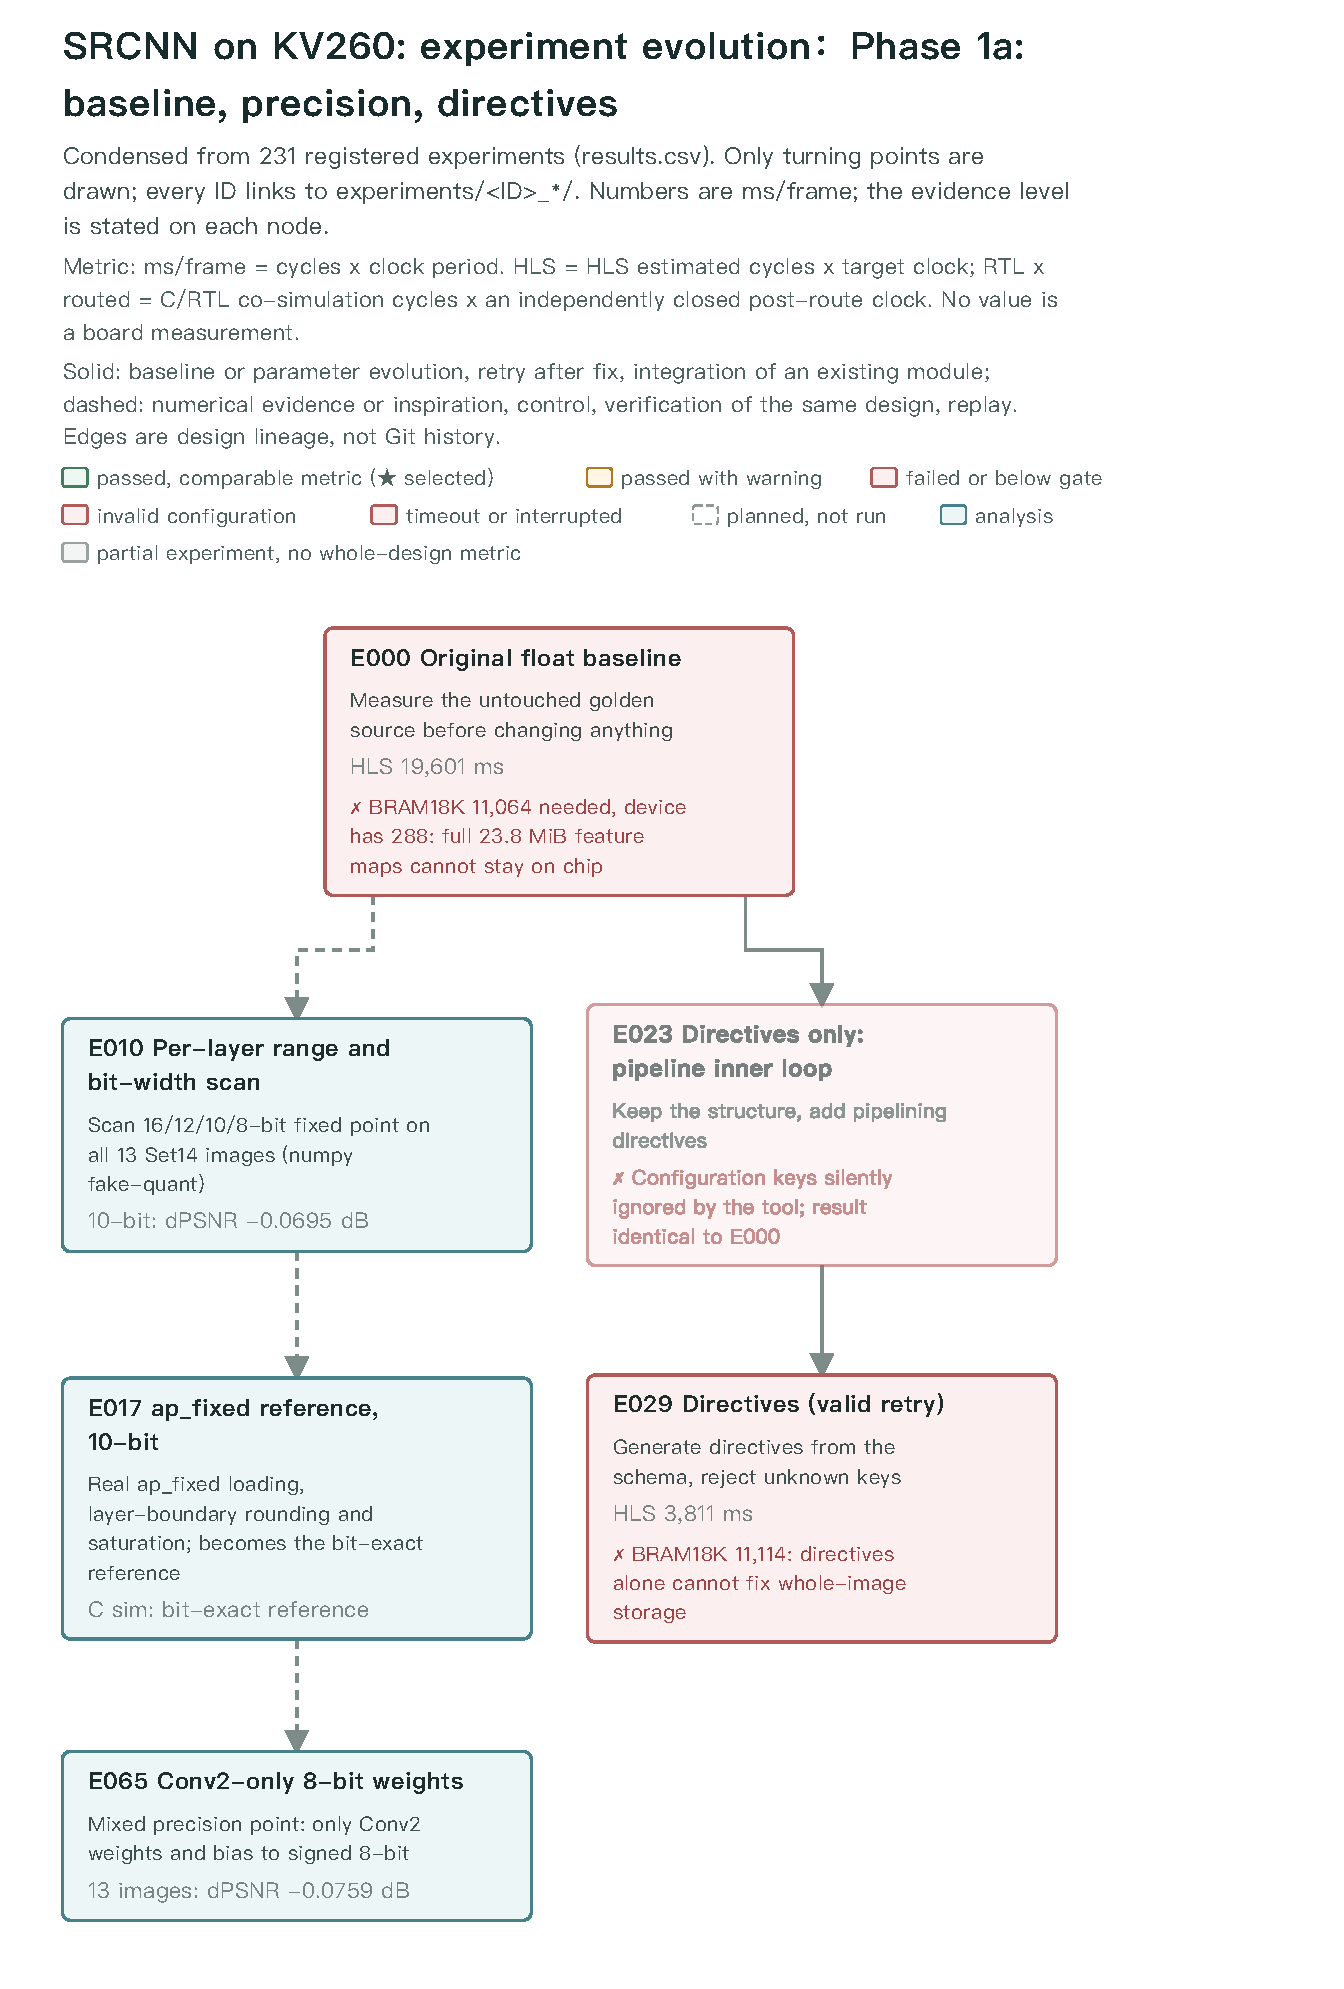
\includegraphics[width=\linewidth,height=0.93\textheight,keepaspectratio]{figures/evolution/baseline.pdf}
% \caption{Phase 1a: baseline, precision and directives. The original float source (E000), the
% precision scan that fixed 10-bit weights and activations (E010), the bit-exact
% \texttt{ap\_fixed} reference (E017) and the directive-only attempts that showed the original
% code cannot fit regardless of pragmas (E020 to E032).}
% \label{fig:evo-baseline}
% \end{figure}

% \begin{figure}[p]
% \centering
% 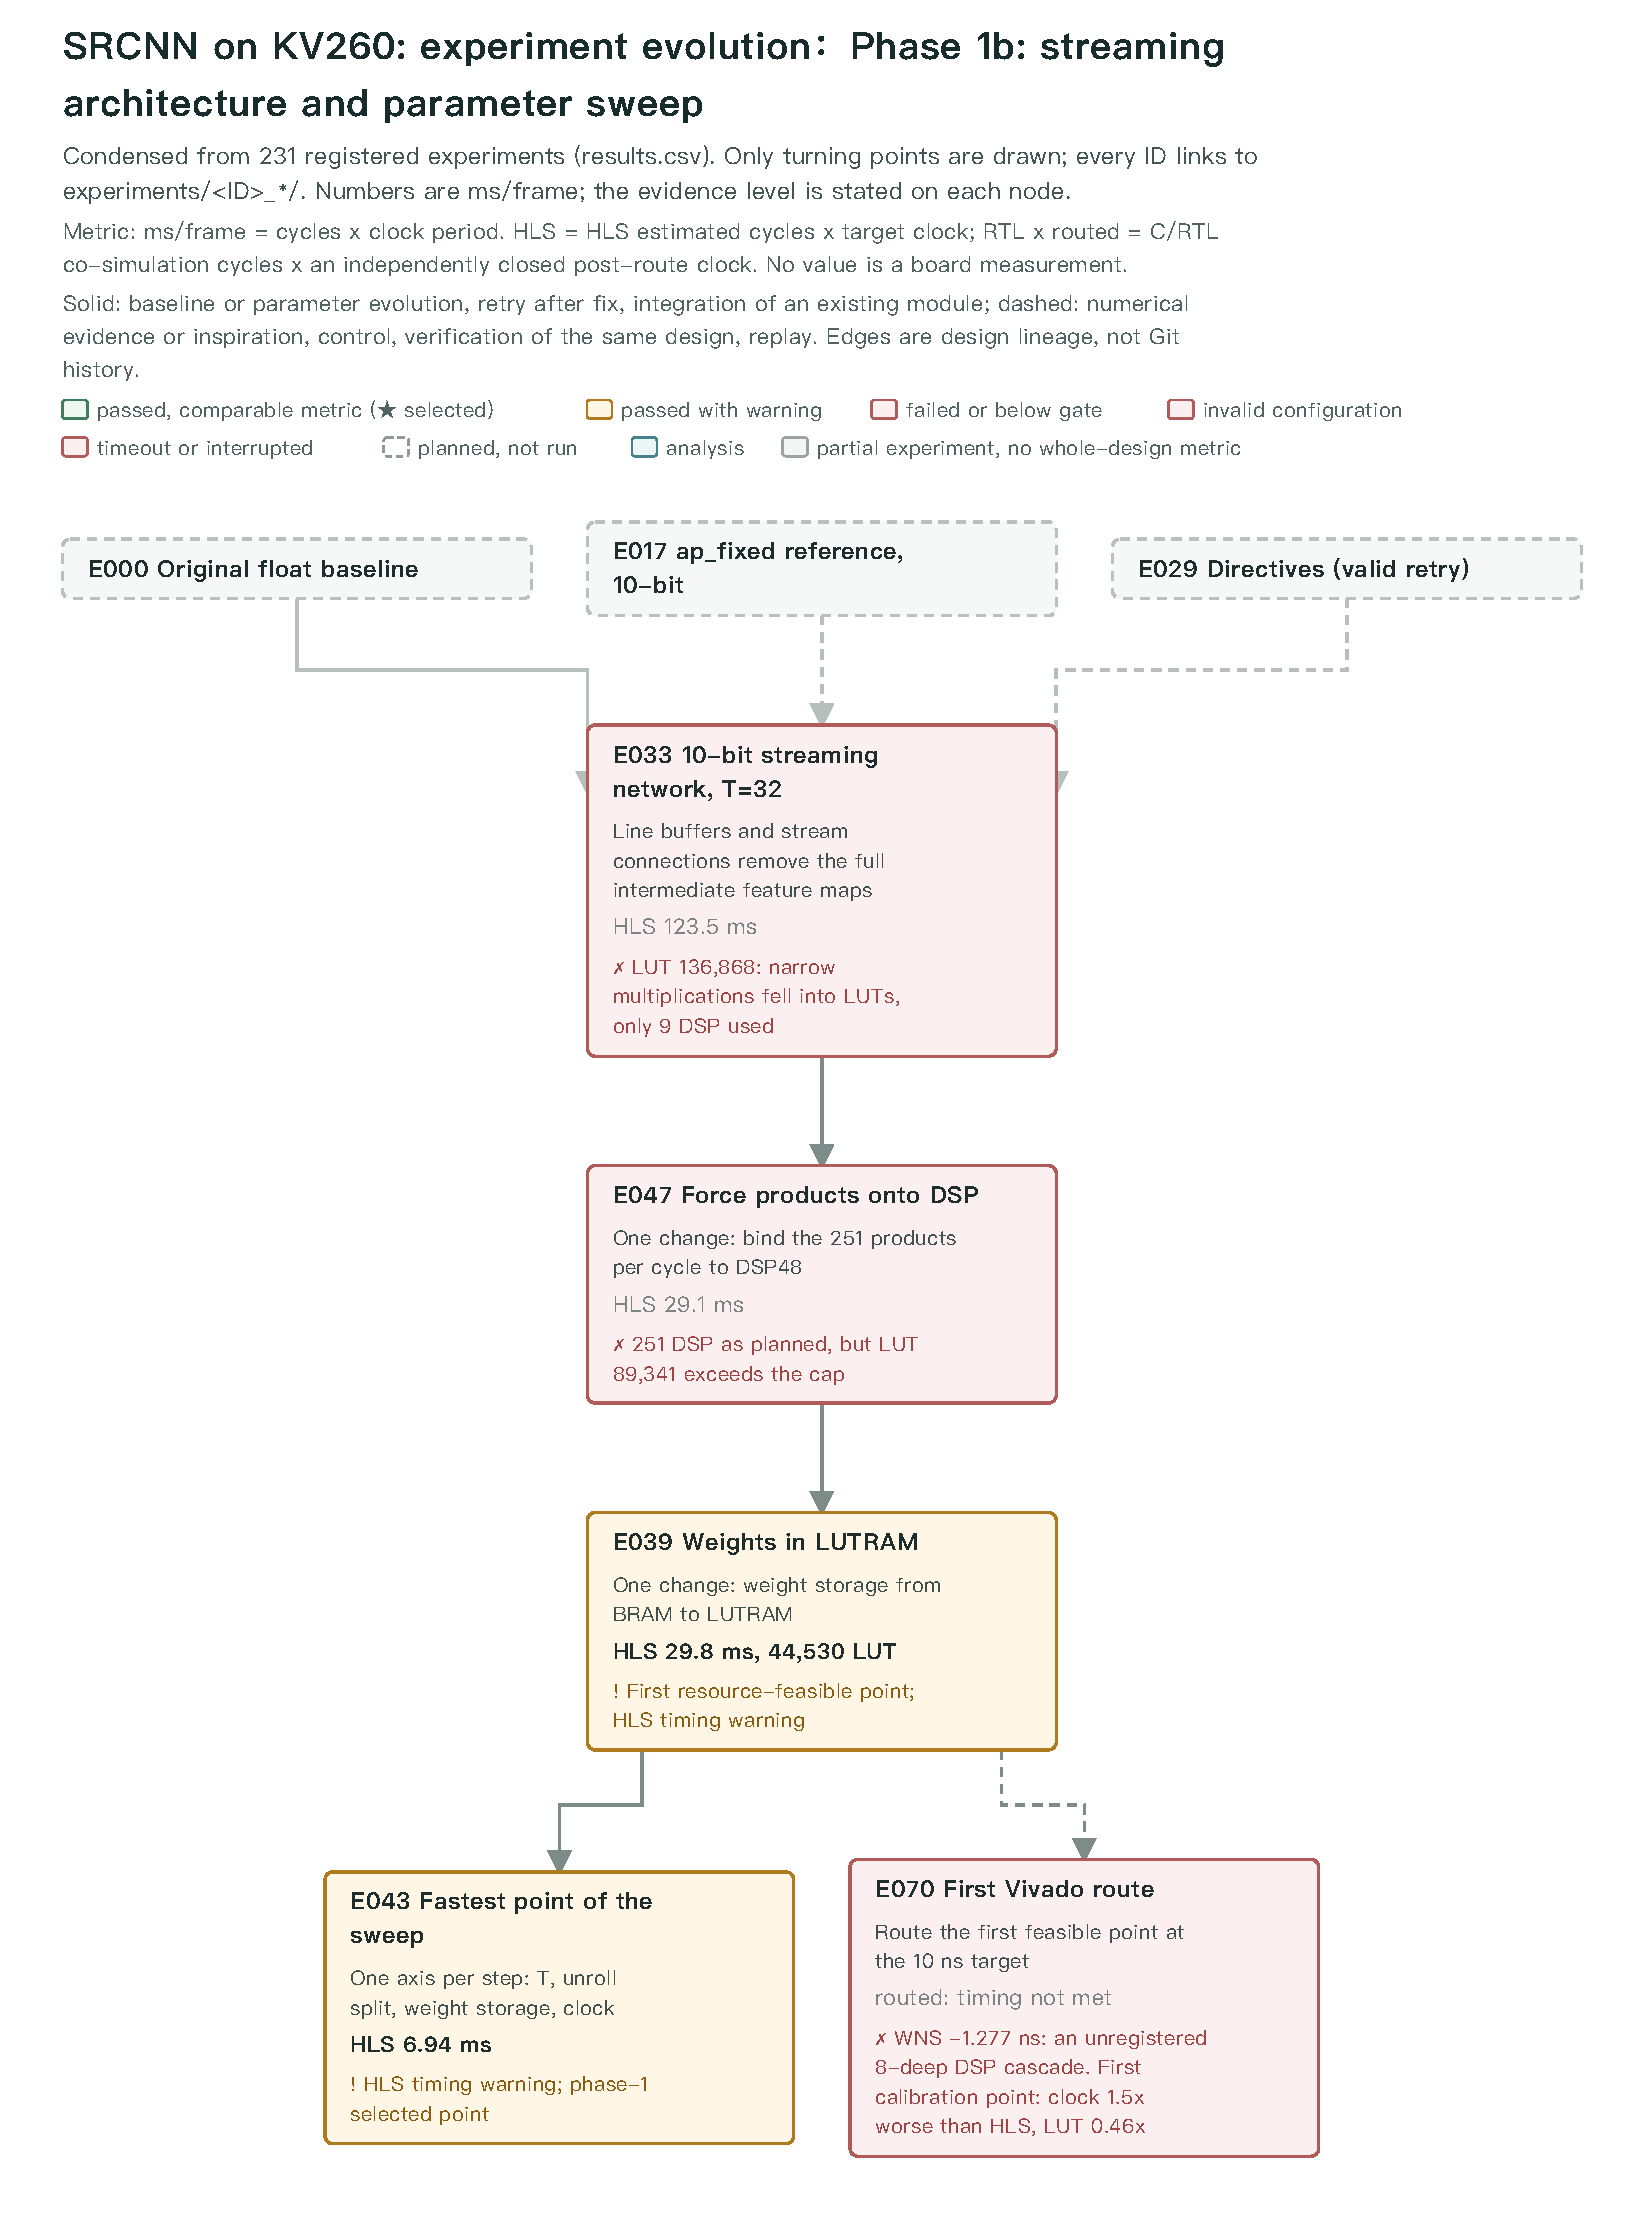
\includegraphics[width=\linewidth,height=0.93\textheight,keepaspectratio]{figures/evolution/stream.pdf}
% \caption{Phase 1b: streaming architecture and parameter sweep. Line buffers and stream
% connections replace the full intermediate feature maps (E033), the products are bound to DSPs
% (E047), the weights move to LUTRAM (E039), and the fold and clock target are swept (E043).}
% \label{fig:evo-stream}
% \end{figure}

% \begin{figure}[p]
% \centering
% 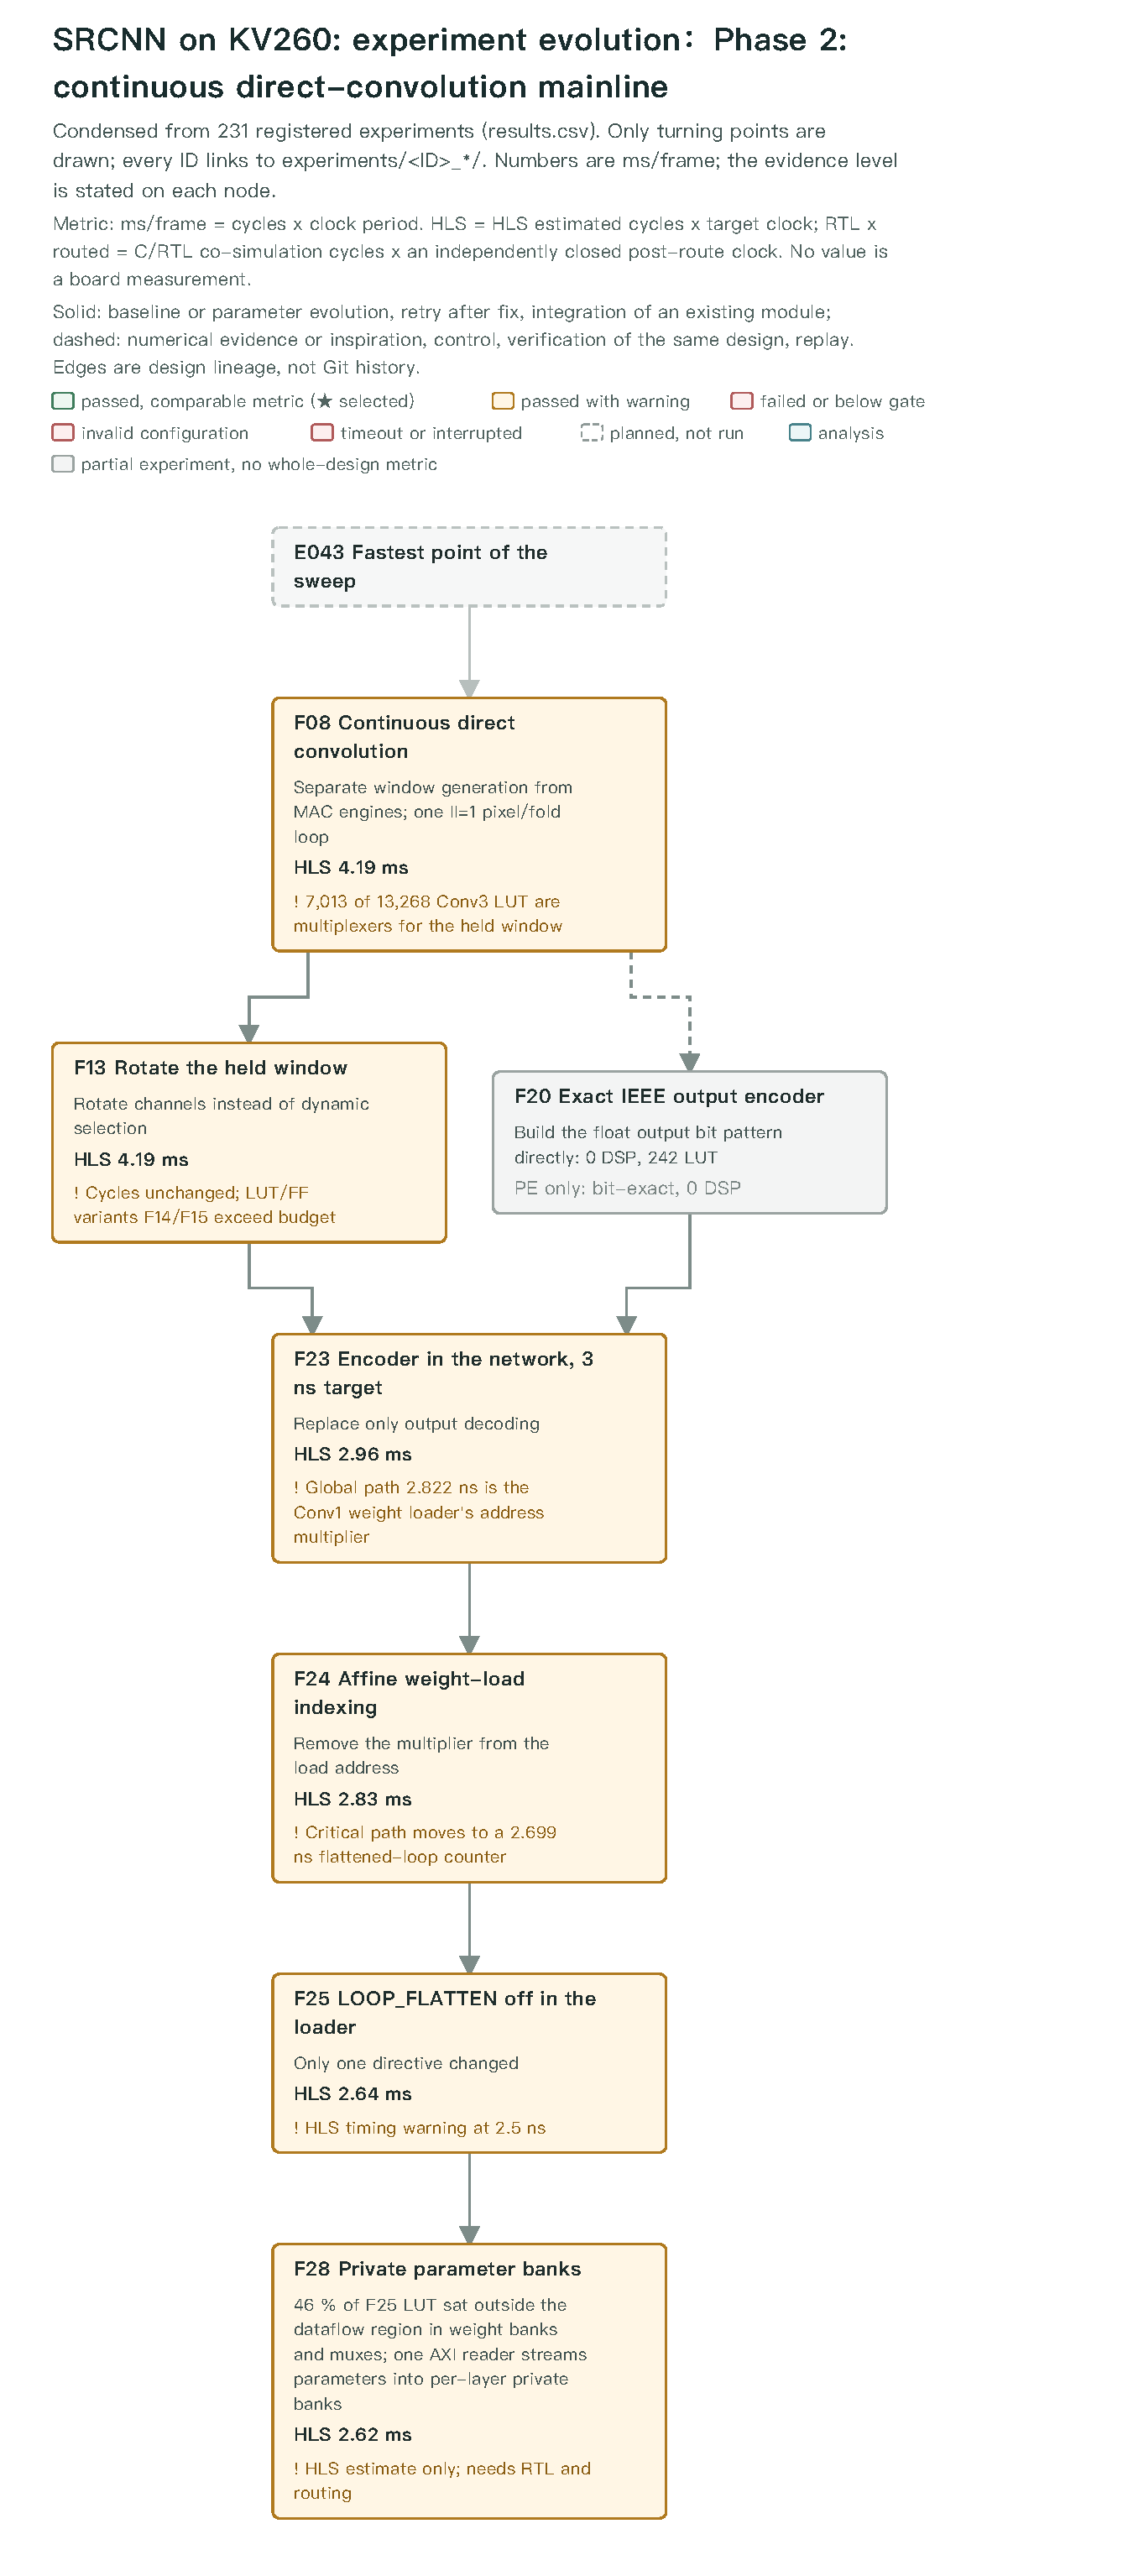
\includegraphics[width=\linewidth,height=0.93\textheight,keepaspectratio]{figures/evolution/mainline.pdf}
% \caption{Phase 2: the continuous direct-convolution mainline. Window generation is separated
% from the MAC engines (F08), the window multiplexers are removed (F13), the output encoder is
% made exact (F20), and the parameter loader is moved off the critical path (F23 to F28).}
% \label{fig:evo-mainline}
% \end{figure}

\begin{figure}[p]
\centering
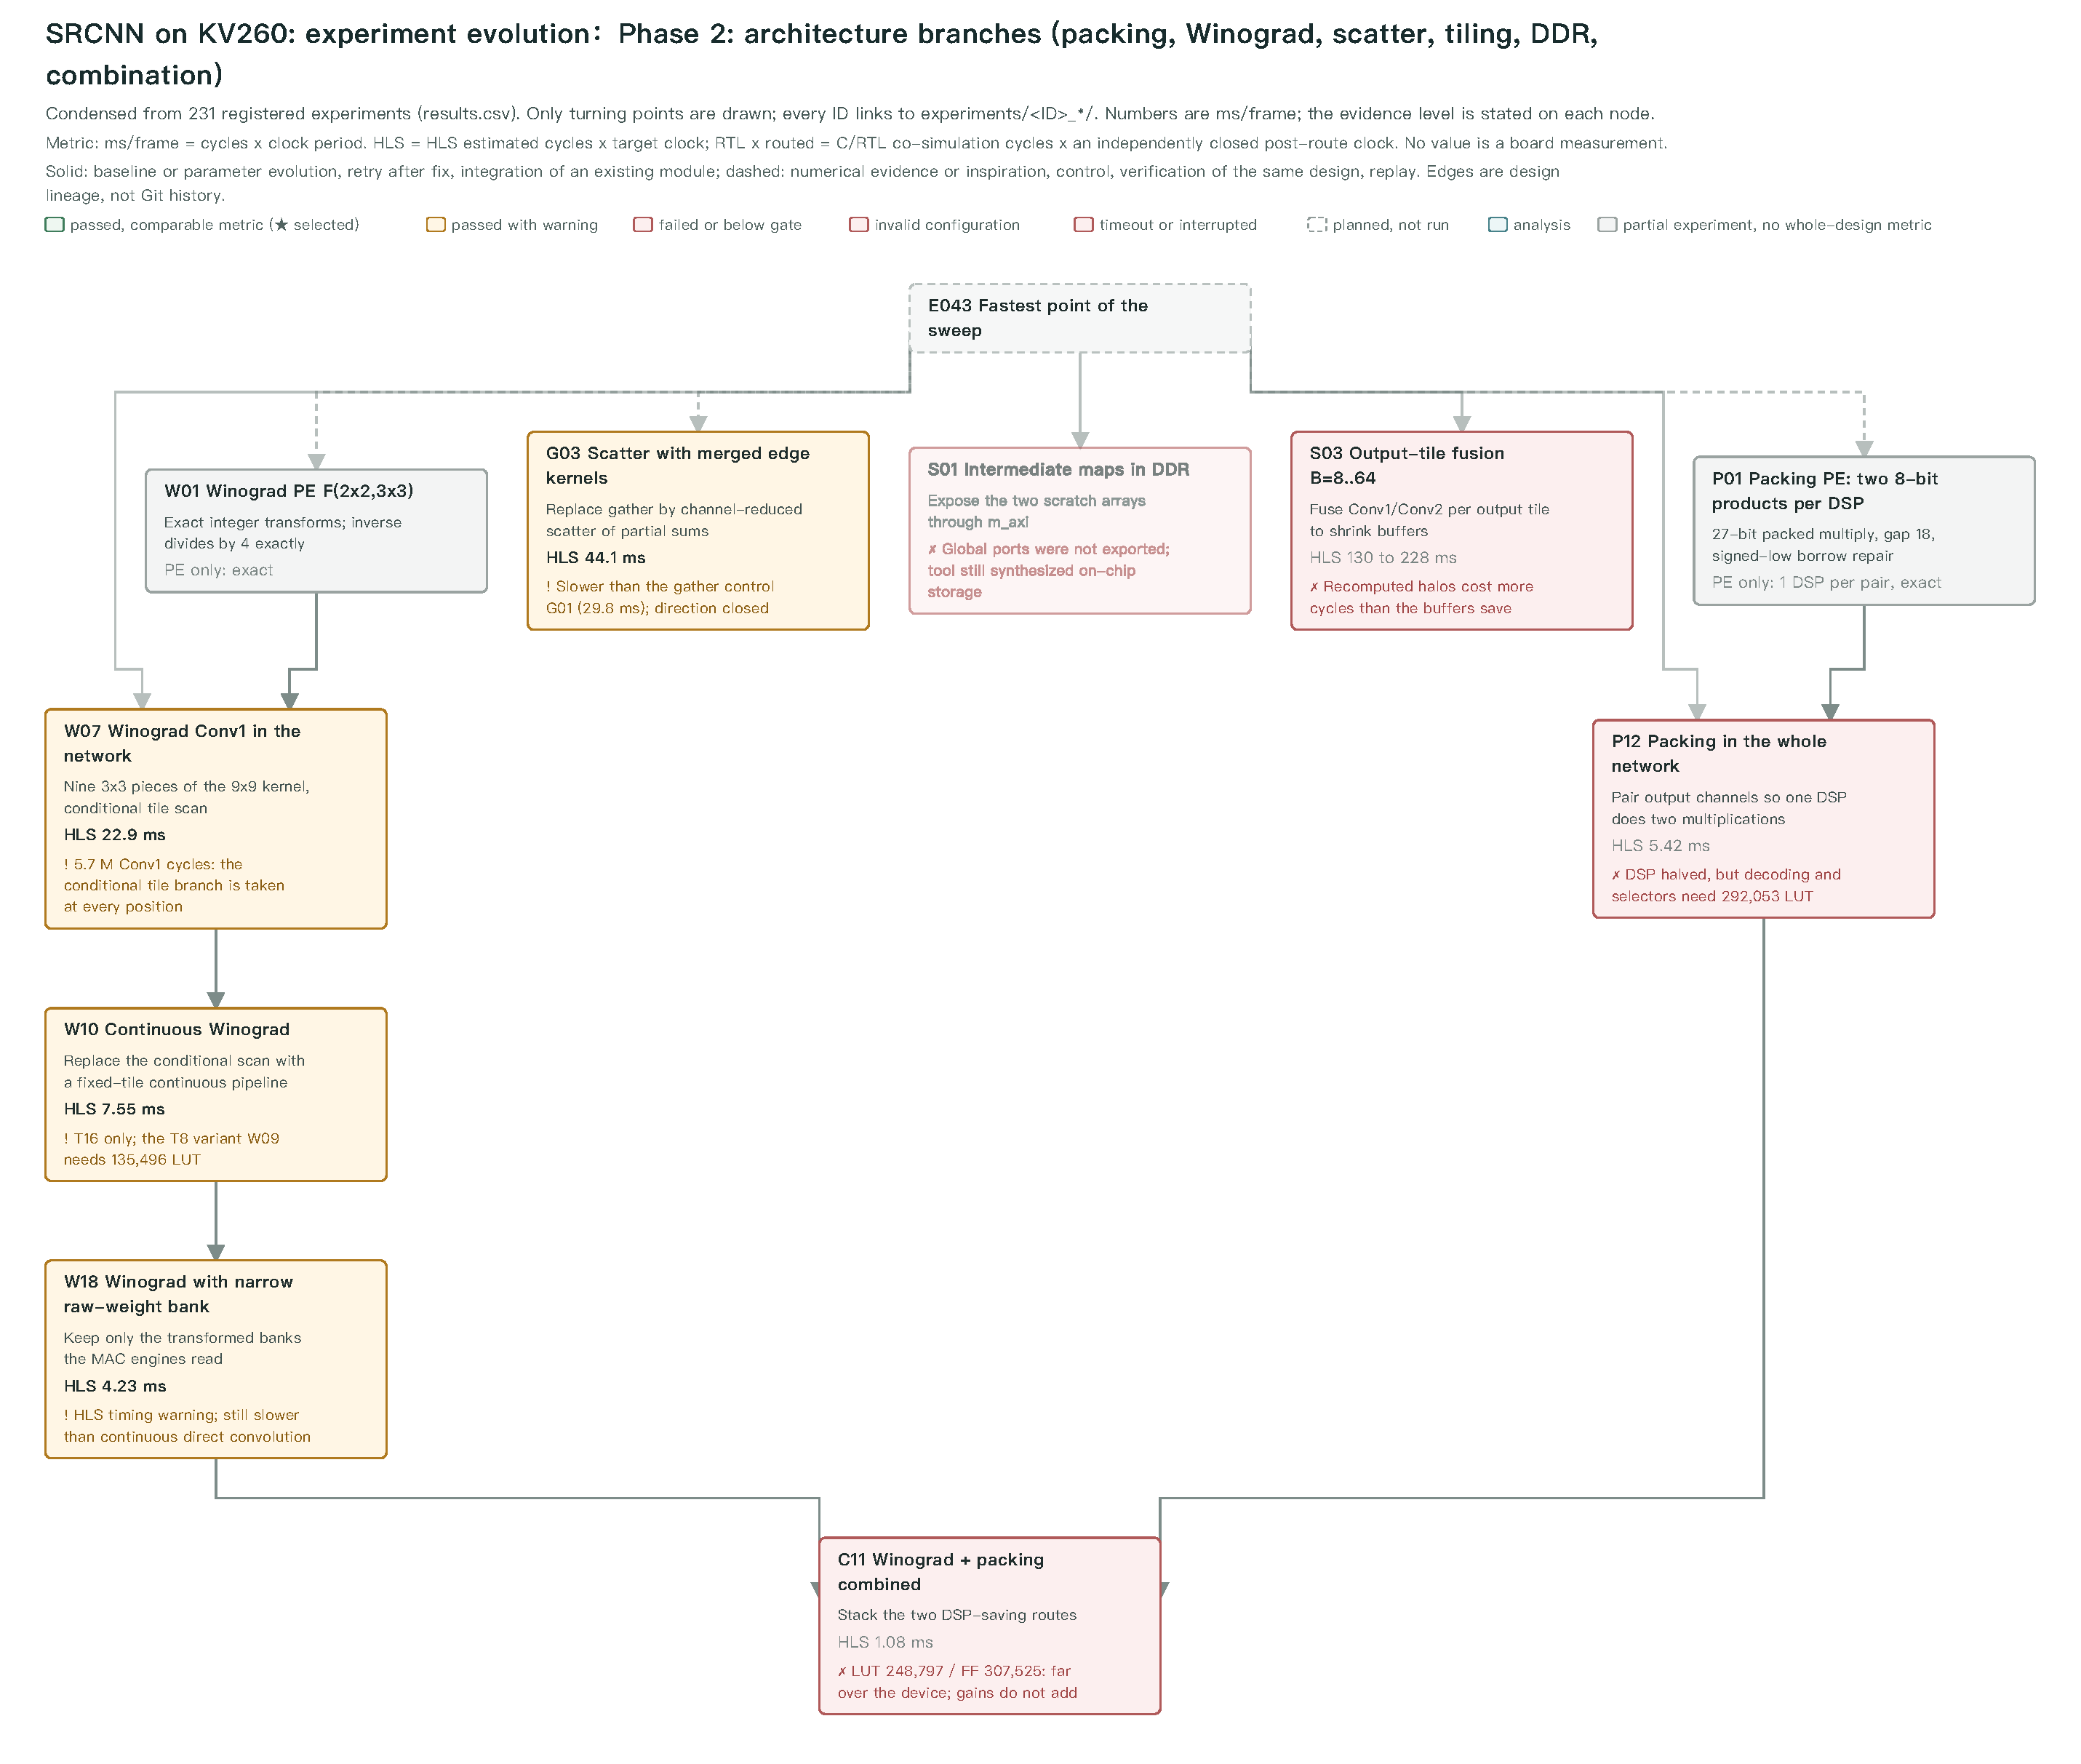
\includegraphics[width=\linewidth,height=0.93\textheight,keepaspectratio]{figures/evolution/branches.pdf}
\caption{Phase 2: architecture branches explored against the mainline: DSP packing (P
series), Winograd (W series), Conv3 scatter (G series), tile fusion and DDR scratch buffers (S
series) and their first combinations (C series).}
\label{fig:evo-branches}
\end{figure}

% \begin{figure}[p]
% \centering
% 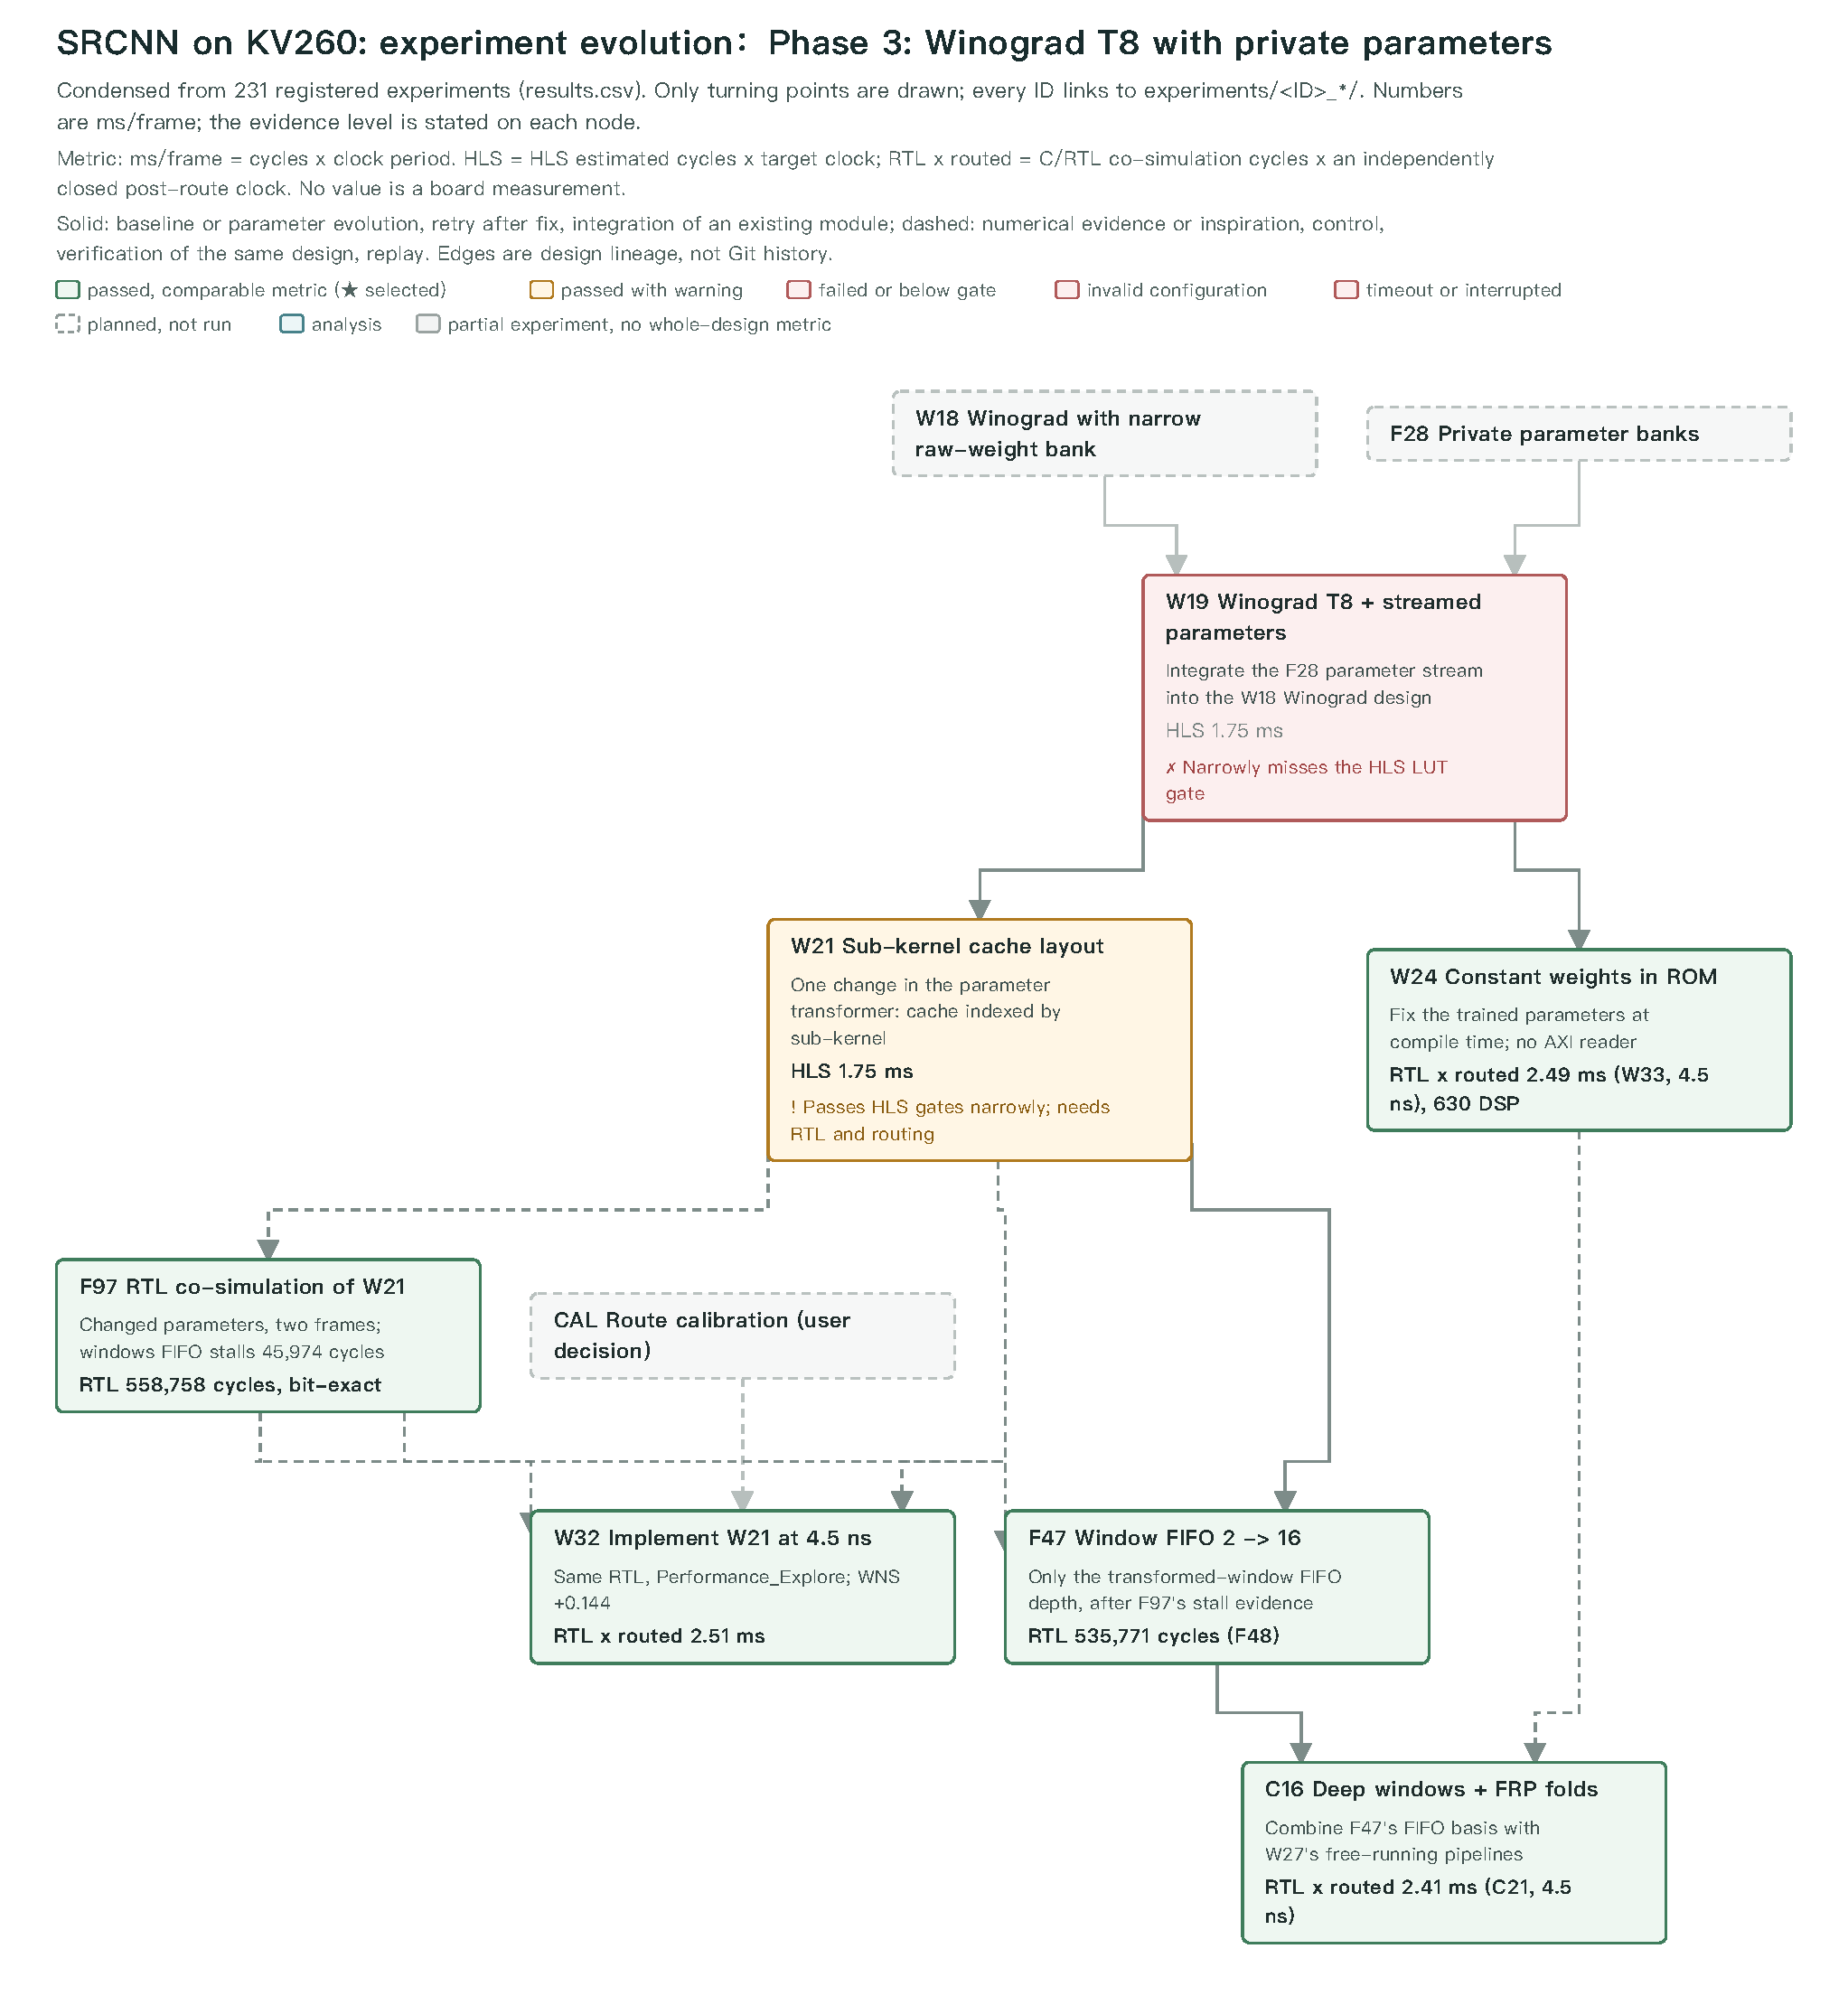
\includegraphics[width=\linewidth,height=0.93\textheight,keepaspectratio]{figures/evolution/winograd.pdf}
% \caption{Phase 3: Winograd at T = 8 with private parameters. The streamed-parameter loader is
% integrated into the Winograd design (W19 to W21), co-simulated (F97) and routed (W32); the
% window-FIFO stall found in F97 leads to F47.}
% \label{fig:evo-winograd}
% \end{figure}

% \begin{figure}[p]
% \centering
% 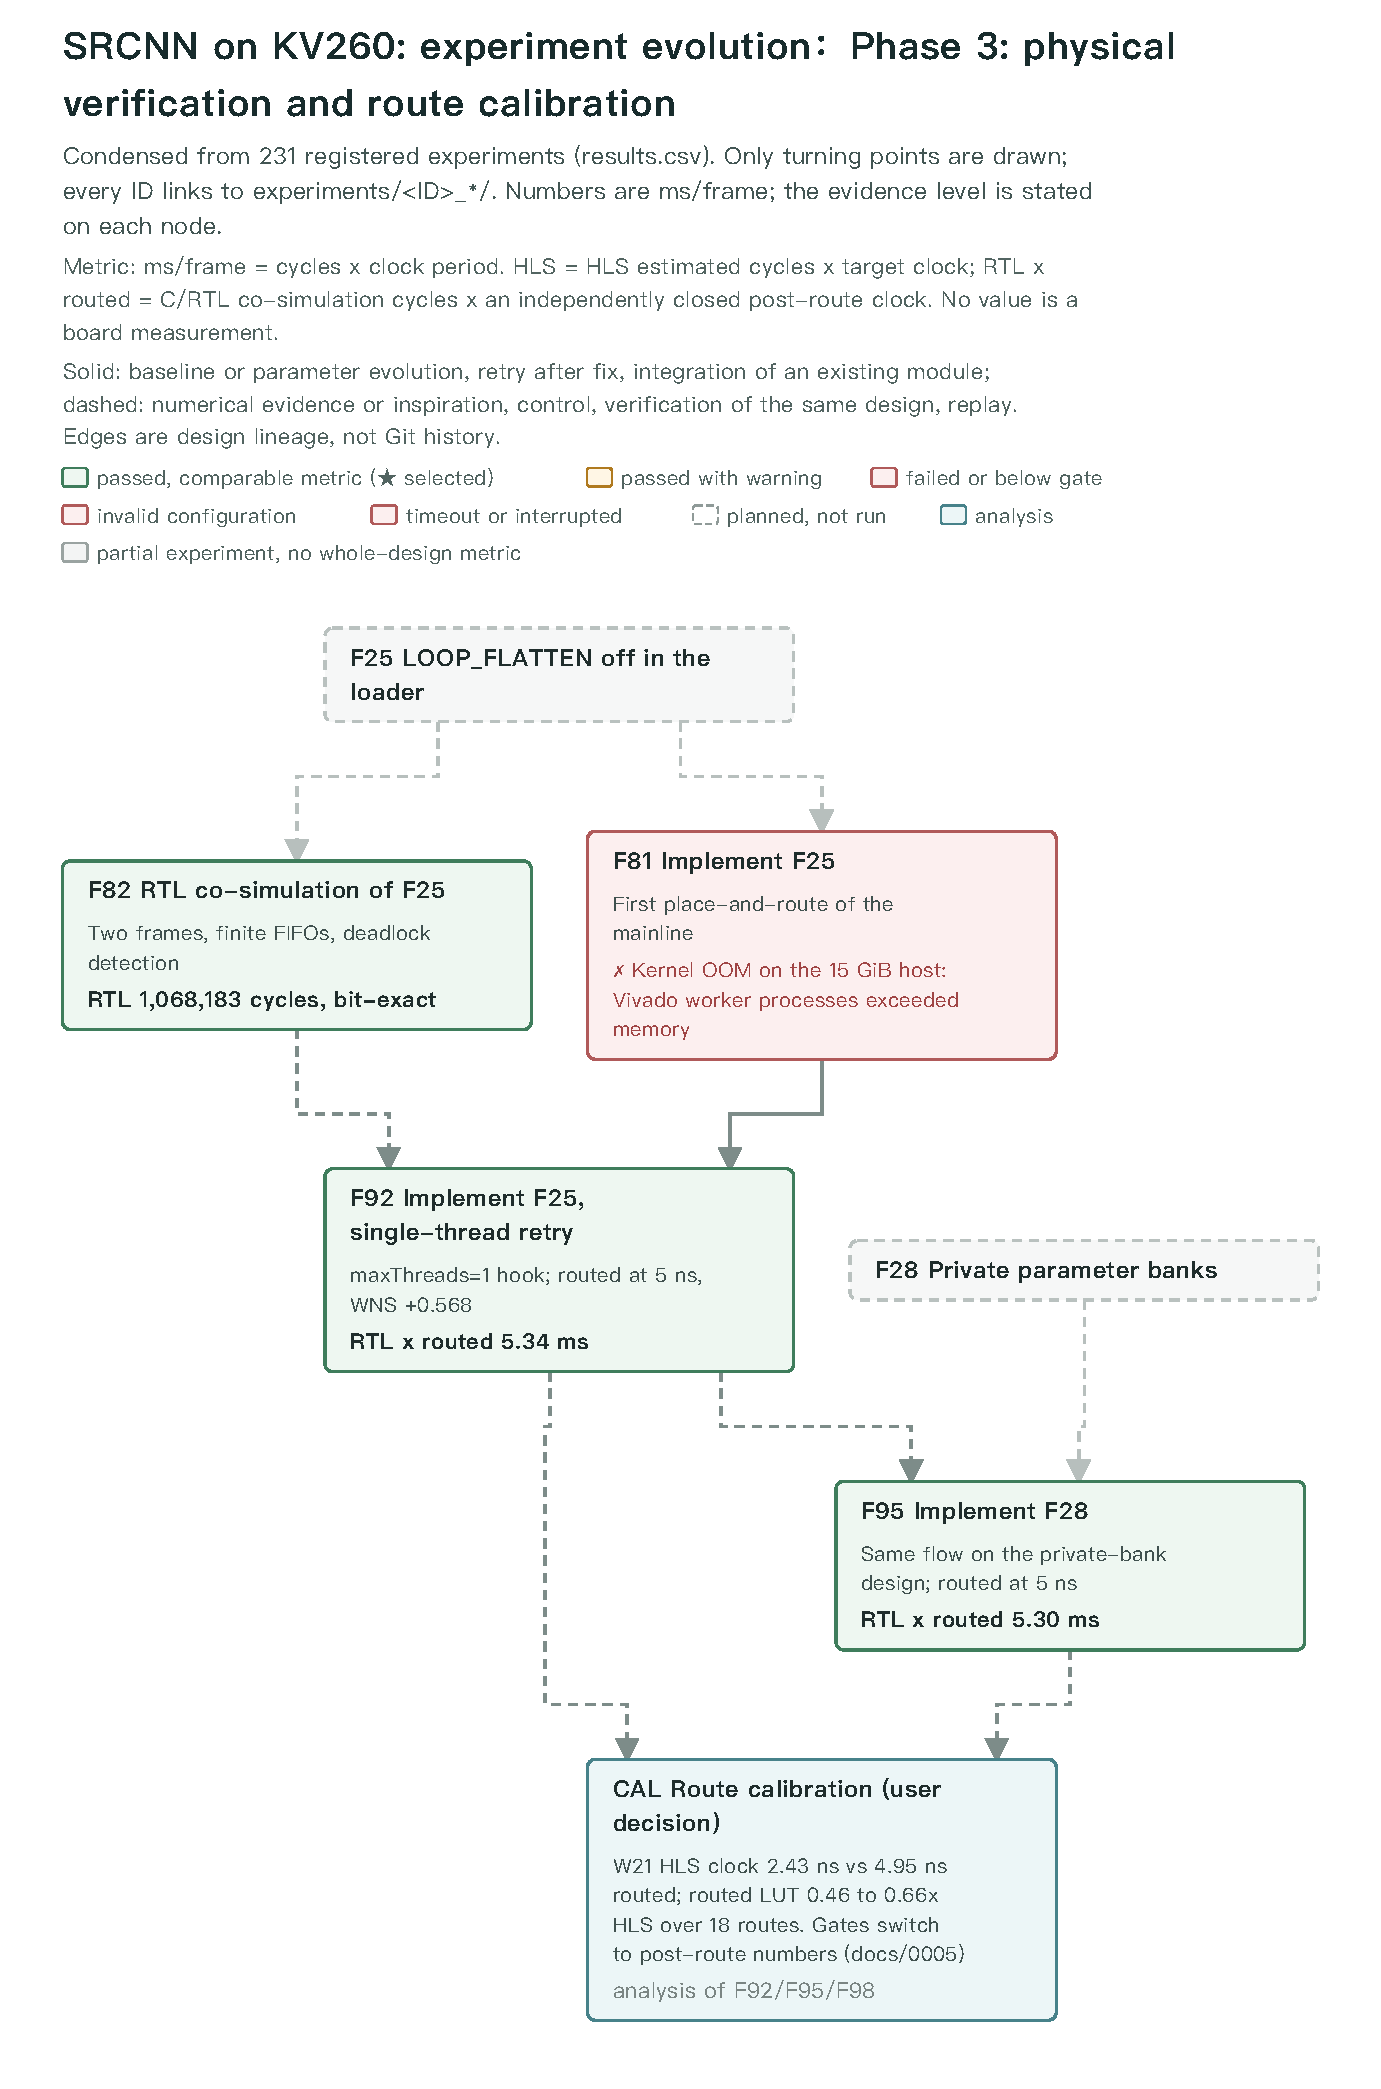
\includegraphics[width=\linewidth,height=0.93\textheight,keepaspectratio]{figures/evolution/physical.pdf}
% \caption{Phase 3: physical verification and route calibration. The first implementations of
% the mainline (F81, F92), the out-of-memory failures that set the host policy, and the routed
% results whose comparison with the HLS estimates changed the gates on 2026-10-12.}
% \label{fig:evo-physical}
% \end{figure}

\begin{figure}[p]
\centering
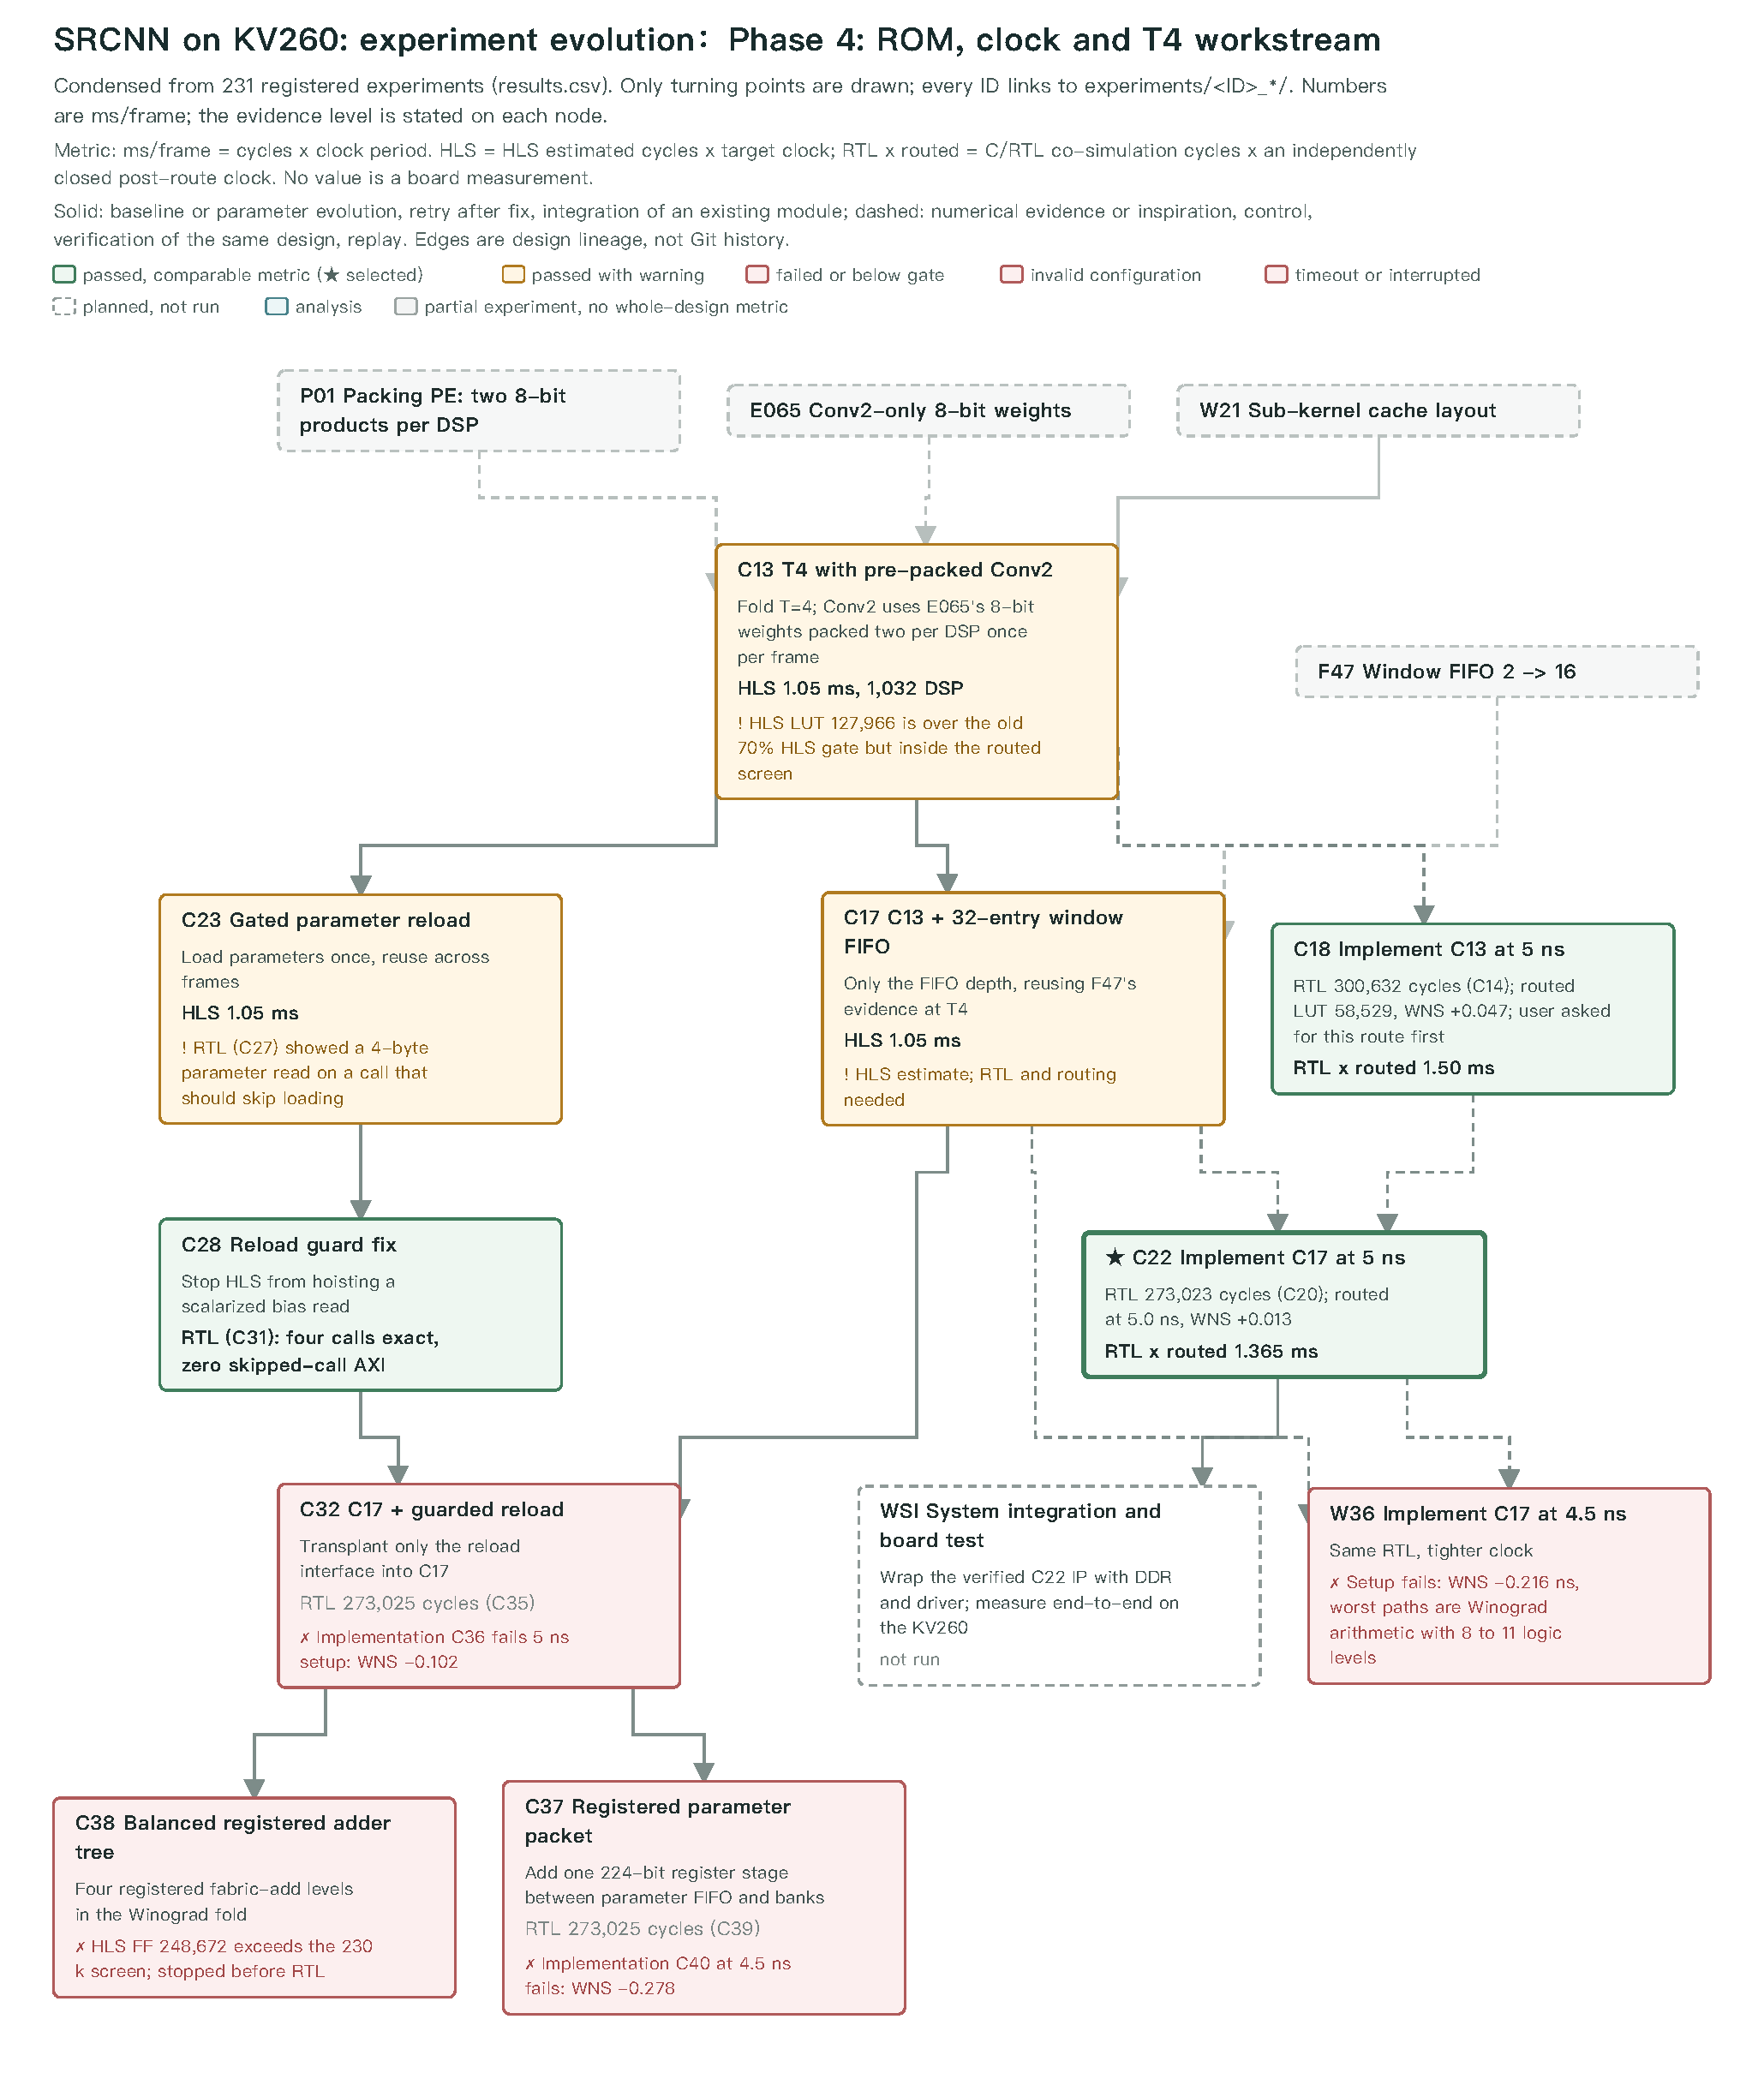
\includegraphics[width=\linewidth,height=0.93\textheight,keepaspectratio]{figures/evolution/t4.pdf}
\caption{Phase 4: ROM parameters, clock and the T = 4 workstream. The pre-packed Conv2
weights make T = 4 fit (C13), the window FIFO is deepened (C17), and the design is
co-simulated (C20) and routed (C18, C22); the attempts at 4.5 ns (W36, C36, C40) fail timing in
the Winograd arithmetic.}
\label{fig:evo-t4}
\end{figure}


\clearpage
\section{The experiment-exploration skill}\label{app:skill}
The agents worked under the project rules file (\texttt{AGENTS.md}, Figure~\ref{fig:1}) and the
reusable skill reproduced below, which they load at the start of every session. It is the
English edition of the skill as it stood at the end of the project (\texttt{SKILL.md} of
\texttt{experiment-exploration-en}); the Chinese original is kept in sync with it. The
templates and the graph-rendering script it refers to are distributed with the skill and are
not reproduced here; its section numbers (1 to 9) correspond to B.1 to B.9 below.
% Generated from SKILL.md by tools/build_skill_appendix.py; do not edit by hand.
English edition of the \passthrough{\lstinline!experiment-exploration!}
skill; keep the two in sync.

This approach comes from the SRCNN FPGA optimization in
\passthrough{\lstinline!\~/School/Hardware/remote/90096\_CNN\_FPGA!}:
170+ experiments, each traceable to its experiment card, raw reports,
and commit. Scripts and templates live in this skill's directory
(\passthrough{\lstinline!scripts/!},
\passthrough{\lstinline!templates/!}).

Division of labor with other skills:

\begin{itemize}
\tightlist
\item
  This skill covers the phase where you don't yet know which approach
  works. Experiment code lives on experiment branches and in independent
  copies, never on the mainline; once an approach is chosen, implement
  it properly following
  \passthrough{\lstinline!production-engineering!}.
\item
  For experiments on n08 / n09, follow
  \passthrough{\lstinline!lab-gpu-servers!} for connecting, picking
  GPUs, and moving data.
\end{itemize}

\subsection{Before starting: write the exploration
plan}

Create an exploration plan under \passthrough{\lstinline!docs/!} from
the template
\passthrough{\lstinline!templates/plan.md!}.
Fill in the following before the first experiment:

\begin{enumerate}
\def\labelenumi{\arabic{enumi}.}
\tightlist
\item
  \textbf{Problem and invariant contract}: what must not change
  (interfaces, data formats, numeric precision, test set). If these
  change, it is no longer the same problem.
\item
  \textbf{A single primary metric}: one number compares every approach,
  with the conversion formula fixed in writing
  (e.g.~\passthrough{\lstinline!ms/image = cycles × clock period (ns) / 10\^6!}).
  Numbers measured on different bases are not ranked together; when they
  must appear side by side, label the basis.
\item
  \textbf{Gates}, in three kinds:

  \begin{itemize}
  \tightlist
  \item
    Quality gate: how correct the result must be (e.g.~\(\Delta\)PSNR
    \(\ge\) \$-\$0.1 dB, bit-exact against the reference);
  \item
    Screening gate: whether it is worth taking to the next level of
    verification;
  \item
    Final gate: whether it can be declared ``feasible''. Only approaches
    that pass the final gate enter the ranking.
  \end{itemize}
\item
  \textbf{Evidence levels}: list your domain's evidence from weakest to
  strongest, e.g.~``paper estimate \textless{} local / unit experiment
  \textless{} simulation \textless{} synthesis estimate \textless{}
  implementation \textless{} hardware measurement''. Tag every
  conclusion with the level it has reached; never present lower-level
  evidence as higher-level.
\item
  \textbf{Numbering scheme}: series prefixes by direction (e.g.~E for
  baseline and sweeps, P / W / G for individual optimization directions,
  C for combinations, F for the mainline); IDs are never reused; reserve
  a separate range for replays (e.g.~100 and above).
\item
  \textbf{Budget and stop rules}: timeout per run; maximum time on any
  one problem (e.g.~45 minutes), after which you stop and record;
  concurrency and memory rules for the machines.
\item
  \textbf{Protected artifacts}: baseline source, data, reference
  outputs. Record their sha256 before starting and verify again at
  wrap-up.
\item
  \textbf{User decisions}: record them in the plan with dates. When a
  new decision supersedes an old rule, keep the old rule as history;
  don't rewrite it.
\end{enumerate}

\subsection{Lifecycle of one
experiment}

\begin{longtable}[]{@{}
  >{\raggedright\arraybackslash}p{(\linewidth - 2\tabcolsep) * \real{0.28}}
  >{\raggedright\arraybackslash}p{(\linewidth - 2\tabcolsep) * \real{0.72}}@{}}
\toprule\noalign{}
\begin{minipage}[b]{\linewidth}\raggedright
Step
\end{minipage} & \begin{minipage}[b]{\linewidth}\raggedright
What to do
\end{minipage} \\
\midrule\noalign{}
\endhead
\bottomrule\noalign{}
\endlastfoot
1. Assign an ID & Confirm it is unused. Completed IDs are never reused;
a rerun after a fix also gets a new ID, linked back with a
\passthrough{\lstinline!retry!} relation \\
2. Write and commit the experiment card &
\passthrough{\lstinline!templates/experiment.json!}:
purpose, control experiment, \textbf{the only thing changed} relative to
the control, conditions held fixed, paper estimate and its basis, how it
will be judged, and what each possible outcome leads to next.
\textbf{Commit first, then run} \\
3. Run in isolation & Copy an independent design or codebase from the
control; don't touch files of completed experiments; no concurrent runs
in the same working directory; every run has a timeout and a log \\
4. Archive & \passthrough{\lstinline!experiments/<id>\_<short-name>/!}:
a copy of the card, raw logs, raw reports, parsed metrics, a one-page
note (result, deviation from the estimate, conclusion), plus the source
commit and tool versions \\
5. Register & The registry \passthrough{\lstinline!results.csv!} is
appended by the parsing script, never by hand; leave unmeasured values
blank, not 0; failures, timeouts, and invalid configurations get a row
too \\
6. Record & Append an entry to \passthrough{\lstinline!LOG.md!}; update
the current state in \passthrough{\lstinline!PROGRESS.md!} \\
7. Commit & One commit per experiment, message starting with the ID,
e.g.~\passthrough{\lstinline!F25 nested\_weight\_loader!} \\
8. Update the evolution graph & Add the node and relations to
\passthrough{\lstinline!graph.json!} and regenerate the SVGs (section
6) \\
\end{longtable}

Completed experiments are immutable: to reproduce one, assign a new ID,
copy the archived design, and rerun it with the recorded commands.

\subsection{When proposing an
optimization}

\begin{enumerate}
\def\labelenumi{\arabic{enumi}.}
\tightlist
\item
  \textbf{Find the bottleneck first, with evidence}: a specific line
  from a report or profile, e.g.~``the 2.822 ns global critical path
  sits on the 15-bit address multiply in Conv1 weight loading''. No
  experiment is opened on an evidence-free ``this should be faster''.
\item
  \textbf{State a testable hypothesis}: ``Changing X should move the
  metric from a to b, because \ldots; the likely cost is \ldots{}''.
\item
  \textbf{Pick a control and change only this one thing}: name the
  control experiment and write the difference in the card's
  \passthrough{\lstinline!changes!}. Change several factors at once and
  you can't tell which one mattered.
\item
  \textbf{Commit the paper estimate first}: write the estimate and its
  basis into the card and commit before running, so it can't be revised
  after the fact.
\item
  \textbf{Compare the measurement with the estimate}: when they differ a
  lot, first explain why (where the estimate went wrong), then decide
  the next step.
\item
  \textbf{Turn the conclusion into a next step}: adopt as the new
  baseline, keep as a branch, or stop, and say why.
\item
  \textbf{Update the evolution graph}.
\end{enumerate}

Rules of judgment:

\begin{itemize}
\tightlist
\item
  Measure the baseline and fix the numeric contract before optimizing.
\item
  Sweep one parameter dimension at a time, round by round; don't change
  every parameter at once.
\item
  Local results (a unit, a single layer, a small kernel) don't
  extrapolate to the whole system.
\item
  Gains from two approaches don't simply add up; a combination must be
  measured on its own.
\item
  The fastest point that fails a gate stays out of the ranking, e.g.~a
  combination with the lowest latency but three times the LUT budget.
\item
  Failure is a result: keep the node and state the cause. Distinguish
  ``configuration didn't take effect'' (invalid: fix and retry) from
  ``valid but below the bar'' (a conclusion).
\item
  A tool ``exiting successfully'' doesn't mean the result is correct;
  check the actual metrics.
\item
  When one problem hits its budget, stop, record the current state, and
  switch direction or ask the user.
\end{itemize}

\subsection{File layout}

\begin{lstlisting}
docs/NNNN-<topic>.md            exploration plan; conclusions written at wrap-up
exp/configs/<id>.json           experiment cards (committed before running)
experiments/
  PROGRESS.md                   resume entry point: current state, what's running, next steps, how to resume
  LOG.md                        append-only event log
  results.csv                   registry (script-generated)
  graph.json                    evolution graph data: hand-written ideas and relations
  evolution/                    generated .svg / .mmd (don't edit by hand)
  <id>_<short-name>/            per-experiment archive
\end{lstlisting}

\passthrough{\lstinline!PROGRESS.md!} template:
\passthrough{\lstinline!templates/PROGRESS.md!}.

\subsection{Registry and log}

\textbf{\passthrough{\lstinline!results.csv!}}: one row per experiment,
with at least these columns:

\passthrough{\lstinline!id, time, series, control, changes, status, <primary metric>, <gate-related metrics>, evidence\_level, git\_commit, archive, notes!}

\begin{itemize}
\tightlist
\item
  \passthrough{\lstinline!status!} uses the same values as the evolution
  graph:
  \passthrough{\lstinline!pass / warn / fail / invalid / timeout / planned / analysis / partial!}.
\item
  Predictions stay in the experiment card, never in the registry; the
  registry holds measurements only.
\item
  If a registered result turns out to be wrong, append a correction
  event to LOG.md and fix it in a new experiment; don't rewrite the
  original reports and logs.
\end{itemize}

\textbf{\passthrough{\lstinline!LOG.md!}} is append-only, one line per
entry, with UTC time and IDs:

\begin{lstlisting}
- 2026-10-10T16:52:16Z: E023/E024/E025 invalid: syn.directive silently ignored by the tool. Now generating directives from the schema and rejecting unknown options; retried as E028/E029/E032.
\end{lstlisting}

\subsection{Experiment evolution graph (SVG directed
graph)}

The evolution graph answers three questions: \textbf{what each
experiment builds on, why it was adjusted that way, and how its result
led to the next experiment}. Update it when a new optimization direction
opens, when a phase wraps up, and when reporting to the user.

\textbf{Data}: \passthrough{\lstinline!experiments/graph.json!}.
Hand-write a one-line idea for each experiment and where it came from.
Example:
\passthrough{\lstinline!templates/graph.example.json!};
rendered result:
\passthrough{\lstinline!templates/example-evolution/overview.svg!}.

\begin{lstlisting}
{ "id": "F25", "title": "Disable load-loop flattening", "group": "mainline", "status": "warn",
  "idea": "One change only: LOOP_FLATTEN off", "metric": 2.64, "problem": "Timing warning at 2.5 ns",
  "parents": ["F24"] }
\end{lstlisting}

\textbf{Generate} (requires Node and dagre 0.8.x; see the header of the
script):

\begin{lstlisting}[language=bash]
node <this skill>/scripts/evolution_graph.cjs experiments/graph.json --all \
     --results experiments/results.csv --metric-column latency_ms
node <this skill>/scripts/evolution_graph.cjs experiments/graph.json --all \
     --results experiments/results.csv --metric-column latency_ms --check
\end{lstlisting}

\passthrough{\lstinline!--all!} produces the overview
\passthrough{\lstinline!overview.svg!} plus one graph per route
(\passthrough{\lstinline!group!}); route graphs draw direct sources from
outside the route as grey dashed boxes.
\passthrough{\lstinline!--check!} writes nothing; it only checks the
data rules, node overlap, and whether the generated files are stale.

\textbf{Node statuses}:

\begin{longtable}[]{@{}
  >{\raggedright\arraybackslash}p{(\linewidth - 4\tabcolsep) * \real{0.3333}}
  >{\raggedright\arraybackslash}p{(\linewidth - 4\tabcolsep) * \real{0.3333}}
  >{\raggedright\arraybackslash}p{(\linewidth - 4\tabcolsep) * \real{0.3333}}@{}}
\toprule\noalign{}
\begin{minipage}[b]{\linewidth}\raggedright
status
\end{minipage} & \begin{minipage}[b]{\linewidth}\raggedright
Meaning
\end{minipage} & \begin{minipage}[b]{\linewidth}\raggedright
Requirement
\end{minipage} \\
\midrule\noalign{}
\endhead
\bottomrule\noalign{}
\endlastfoot
\passthrough{\lstinline!pass!} & Passed the current stage, with a
comparable metric & Must have a metric; may add
\passthrough{\lstinline!"selected": true!} to mark the current choice
(\(\star\), bold border) \\
\passthrough{\lstinline!warn!} & Passed with warnings (e.g.~timing
warnings) & Must have a metric; put the warning in
\passthrough{\lstinline!problem!} \\
\passthrough{\lstinline!fail!} & Below the bar, or failed & Must have a
one-line \passthrough{\lstinline!problem!}; any metric is shown only in
grey \\
\passthrough{\lstinline!invalid!} & Invalid configuration (didn't take
effect); faded & Must have \passthrough{\lstinline!problem!} \\
\passthrough{\lstinline!timeout!} & Timed out or interrupted; faded &
Must have \passthrough{\lstinline!problem!} \\
\passthrough{\lstinline!planned!} & Planned, not run; dashed border &
Must not have a metric \\
\passthrough{\lstinline!analysis!} & Software analysis or numeric study
& --- \\
\passthrough{\lstinline!partial!} & Local experiment (unit, single
layer), no whole-system metric & Don't invent a whole-system metric \\
\end{longtable}

\textbf{Relations} (solid lines are design evolution; dashed lines are
evidence and verification):

\begin{longtable}[]{@{}lll@{}}
\toprule\noalign{}
kind & Meaning & Line \\
\midrule\noalign{}
\endhead
\bottomrule\noalign{}
\endlastfoot
\passthrough{\lstinline!source!} & Design or parameter baseline
(default) & solid \\
\passthrough{\lstinline!retry!} & Retry after a fix & solid \\
\passthrough{\lstinline!integrate!} & Integrates an existing module &
solid \\
\passthrough{\lstinline!reference!} & Numeric basis or inspiration &
dashed \\
\passthrough{\lstinline!control!} & Control & dashed \\
\passthrough{\lstinline!verify!} & Verification of the same design &
dashed \\
\passthrough{\lstinline!replay!} & Reproduction & dashed \\
\end{longtable}

\textbf{Drawing rules}:

\begin{itemize}
\tightlist
\item
  Exactly one node per experiment; relations are dependencies between
  ideas, not Git commit history; no cycles.
\item
  An experiment normally links to one primary source; link several only
  when integrating, or when bringing in a key numeric basis.
\item
  Keep failed nodes, with a specific one-line problem such as ``LUT
  248,797, 3\(\times\) over budget'', not just ``failed''.
\item
  Put only the primary metric on a node; resources, accuracy, and other
  details go in the experiment record.
\item
  The registry is the source of truth for metrics: cross-check with
  \passthrough{\lstinline!--results!}, and fix
  \passthrough{\lstinline!graph.json!} when they disagree.
\item
  Once there are many experiments (dozens or more), split them into
  routes by \passthrough{\lstinline!group!} and keep only the trunk in
  the overview; if needed, use route-level summary nodes there.
\end{itemize}

\textbf{Accompanying text}: in the exploration plan or a separate
document, write one paragraph per route answering the three questions
above, and embed the matching SVG. Readers look at the overview first,
then at each route for detail.

\subsection{Resuming and handover}

\begin{itemize}
\tightlist
\item
  \passthrough{\lstinline!PROGRESS.md!} is the resume entry point:
  current branch and baseline, completed IDs, running jobs (machine,
  process, log path), to-dos, user decisions in force, and resume steps.
  Update it at the end of every experiment.
\item
  Check processes before resuming: remote jobs may have finished or may
  still be running. For finished jobs, only collect results
  (collect-only) and don't relaunch them; never start a second copy of a
  job that is still running.
\item
  The handover document states which conclusions have reached which
  evidence level, what hasn't been verified yet, and the candidates for
  the next step with reasons.
\end{itemize}

\subsection{Reporting}

Every report uses a table; write \passthrough{\lstinline!unknown!} for
anything not measured:

\begin{longtable}[]{@{}
  >{\raggedright\arraybackslash}p{(\linewidth - 12\tabcolsep) * \real{0.1429}}
  >{\raggedright\arraybackslash}p{(\linewidth - 12\tabcolsep) * \real{0.1429}}
  >{\raggedright\arraybackslash}p{(\linewidth - 12\tabcolsep) * \real{0.1429}}
  >{\raggedright\arraybackslash}p{(\linewidth - 12\tabcolsep) * \real{0.1429}}
  >{\raggedright\arraybackslash}p{(\linewidth - 12\tabcolsep) * \real{0.1429}}
  >{\raggedright\arraybackslash}p{(\linewidth - 12\tabcolsep) * \real{0.1429}}
  >{\raggedright\arraybackslash}p{(\linewidth - 12\tabcolsep) * \real{0.1429}}@{}}
\toprule\noalign{}
\begin{minipage}[b]{\linewidth}\raggedright
ID
\end{minipage} & \begin{minipage}[b]{\linewidth}\raggedright
What changed vs.~control
\end{minipage} & \begin{minipage}[b]{\linewidth}\raggedright
Primary metric
\end{minipage} & \begin{minipage}[b]{\linewidth}\raggedright
Gate results
\end{minipage} & \begin{minipage}[b]{\linewidth}\raggedright
Evidence level
\end{minipage} & \begin{minipage}[b]{\linewidth}\raggedright
Status
\end{minipage} & \begin{minipage}[b]{\linewidth}\raggedright
Conclusion / next step
\end{minipage} \\
\midrule\noalign{}
\endhead
\bottomrule\noalign{}
\endlastfoot
\end{longtable}

Also state:

\begin{itemize}
\tightlist
\item
  the currently selected approach, and why it is the one;
\item
  deviations from the paper estimates;
\item
  items that haven't reached the final gate yet;
\item
  the path to the evolution graph.
\end{itemize}

\subsection{Subagents and models}

Subagents default to Sonnet; for the setting and the precedence order,
see section 7 of \passthrough{\lstinline!production-engineering!}.

\begin{itemize}
\tightlist
\item
  Good fits for Sonnet subagents: running an experiment from its
  committed experiment card, checking remote jobs and collecting
  results, parsing reports and appending to the registry, generating and
  checking the evolution graph, searching past experiments and logs.
\item
  Pass \passthrough{\lstinline!model: "opus"!} explicitly for: finding
  bottleneck evidence in reports, writing hypotheses and paper
  estimates, explaining gaps between estimates and measurements,
  verifying any claim that something passes the final gate.
\end{itemize}


\clearpage
\section{Readable version of the selected design}\label{app:code-readable}
Flattened version of C17 (\texttt{designs/\allowbreak winograd\_t4\_windows32\_v1}) with the compile-time
macros substituted and the templates expanded, for reading and analysis only. C simulation and
HLS synthesis of this version give the same outputs and the same synthesis results as the original
(Section~\ref{sec:4}).
\lstinputlisting[style=source]{code/C17_readable_srcnn.cpp}

\end{document}
